\documentclass[a4paper,12pt]{report}
%\documentclass[a4paper,12pt,landscape,twocolumn]{report}
\usepackage[a4paper, inner=1.7cm, outer=2.7cm, top=2cm, bottom=2cm,bindingoffset=1.2cm ]{geometry}

\usepackage[english]{babel}

\usepackage{blindtext}
\usepackage{graphicx}
\usepackage{wrapfig}
\usepackage{enumitem}
\usepackage{fancyhdr}
\usepackage{amsmath}
\usepackage{index}
\usepackage{footmisc}
\usepackage{xlop}
\usepackage{tikz}
\usepackage{pstricks}
\usepackage{multido}
\usepackage{color}
\usepackage{pgfplots}
\usepackage{array}
\usepackage{setspace}
\usepackage{siunitx}
%\usepackage[normalem]{ulem}
%\usepackage{soul}
\usepackage{cancel}
\usepackage{tkz-euclide}
\usepackage{placeins}
\usetkzobj{all}
\usetikzlibrary{shapes.geometric}
\usepackage{multicol}
 

\usetikzlibrary{arrows,angles}
\pgfplotsset{compat=1.16,width=10cm}
\usetikzlibrary{quotes,angles,positioning,decorations.pathreplacing, spy}

\pagestyle{fancy}
\makeindex

\newenvironment{myindentpar}[1]
{
	\begin{list}{}
          	{\setlength{\leftmargin}{#1}}
          	\item[]
 }
  {\end{list}}

\def\Dot[#1](#2){\psdot[dotstyle = o, fillcolor = #1](!#2 0)}

\newcolumntype{?}{!{\vrule width 2pt}}



\makeatletter
\def\thickhline{%
  \noalign{\ifnum0=`}\fi\hrule \@height \thickarrayrulewidth \futurelet
   \reserved@a\@xthickhline}
\def\@xthickhline{\ifx\reserved@a\thickhline
               \vskip\doublerulesep
               \vskip-\thickarrayrulewidth
             \fi
      \ifnum0=`{\fi}}
\makeatother

\newlength{\thickarrayrulewidth}
\setlength{\thickarrayrulewidth}{3\arrayrulewidth}




\begin{document}

\title{\Large{\textbf{A Primer On \\Numerical Mathematics}}}
	\author{Dr. Achim Kehrein \\ Dr. Thorsten Camps\\William L. Cole}
	\date{13.08.2019}

	\maketitle
	\tableofcontents

	\pagenumbering{arabic} 
	\setcounter{page}{2}

	\fancyhf{}

\renewcommand{\headrulewidth}{2pt}
\renewcommand{\footrulewidth}{2pt}

\fancyhead[LE]{\leftmark}
	\fancyhead[RO]{\nouppercase{\rightmark}}
	\fancyfoot[LE,RO]{\thepage}

	\renewcommand{\thefootnote}{\fnsymbol{footnote}}

\setcounter{chapter}{-1}
\chapter{Numerical Mathematics: A Paradigm Shift}

% OVERVIEW -------------------------------------------------------------------------------------------------------
\begin{quote}
	"Because most things don't work the same way on a computer - to a scary extent."\\
\end{quote}

\section{A "New" Approach to Math.}


	So far:\\
	Infinite processes (limits, derivatives, integrals, etc.)\\
	$\longmapsto$ Must truncate these processes to make them finite. ("Truncation Error")\\
\\
	Infinitely many numbers, infinite precision:\\
	$\longmapsto$ Computer has only finitely many machine numbers with finite precision ("roundoff 
	error")\\
\\
	Error propagation in mathematical recipes: Mathematically equivalent formulas may produce 
	different results on a computer. Which result is
	more accurate?\\
\\
	Goal of Numerics Course:\\
	Learn to treat each problem individually instead of applying "standard recipes".\\


% DATA TYPES -----------------------------------------------------------------------------------------------------
\chapter{Number Representation in Computers and Calculators}

	Which numbers does a computer use?\\
\\
	Two types:

\begin{itemize}
	\item{INT - Integer}
	\item{FLOAT, DOUBLE - Floating point numbers}\\
\end{itemize}

	In the past, calculators only used FLOATs. Modern Calculators use both INTs and FLOATs.


% INTEGERS --------------------------------------------------------------------------------------------------------
\section{Integers}
	...-1, 0, 1, 2, 3...\\ \\

	Infinitely many in math, but computers can only represent finitely many.\\ \\
	$INT_{MIN}$, $INT_{MIN}$+1, ..., -1, 0, 1, ..., $INT_{MAX}$


\begin{figure}[!htb]
	% r - right
	% l - left
	% o - outside edge
	% i - inside edge
	\center{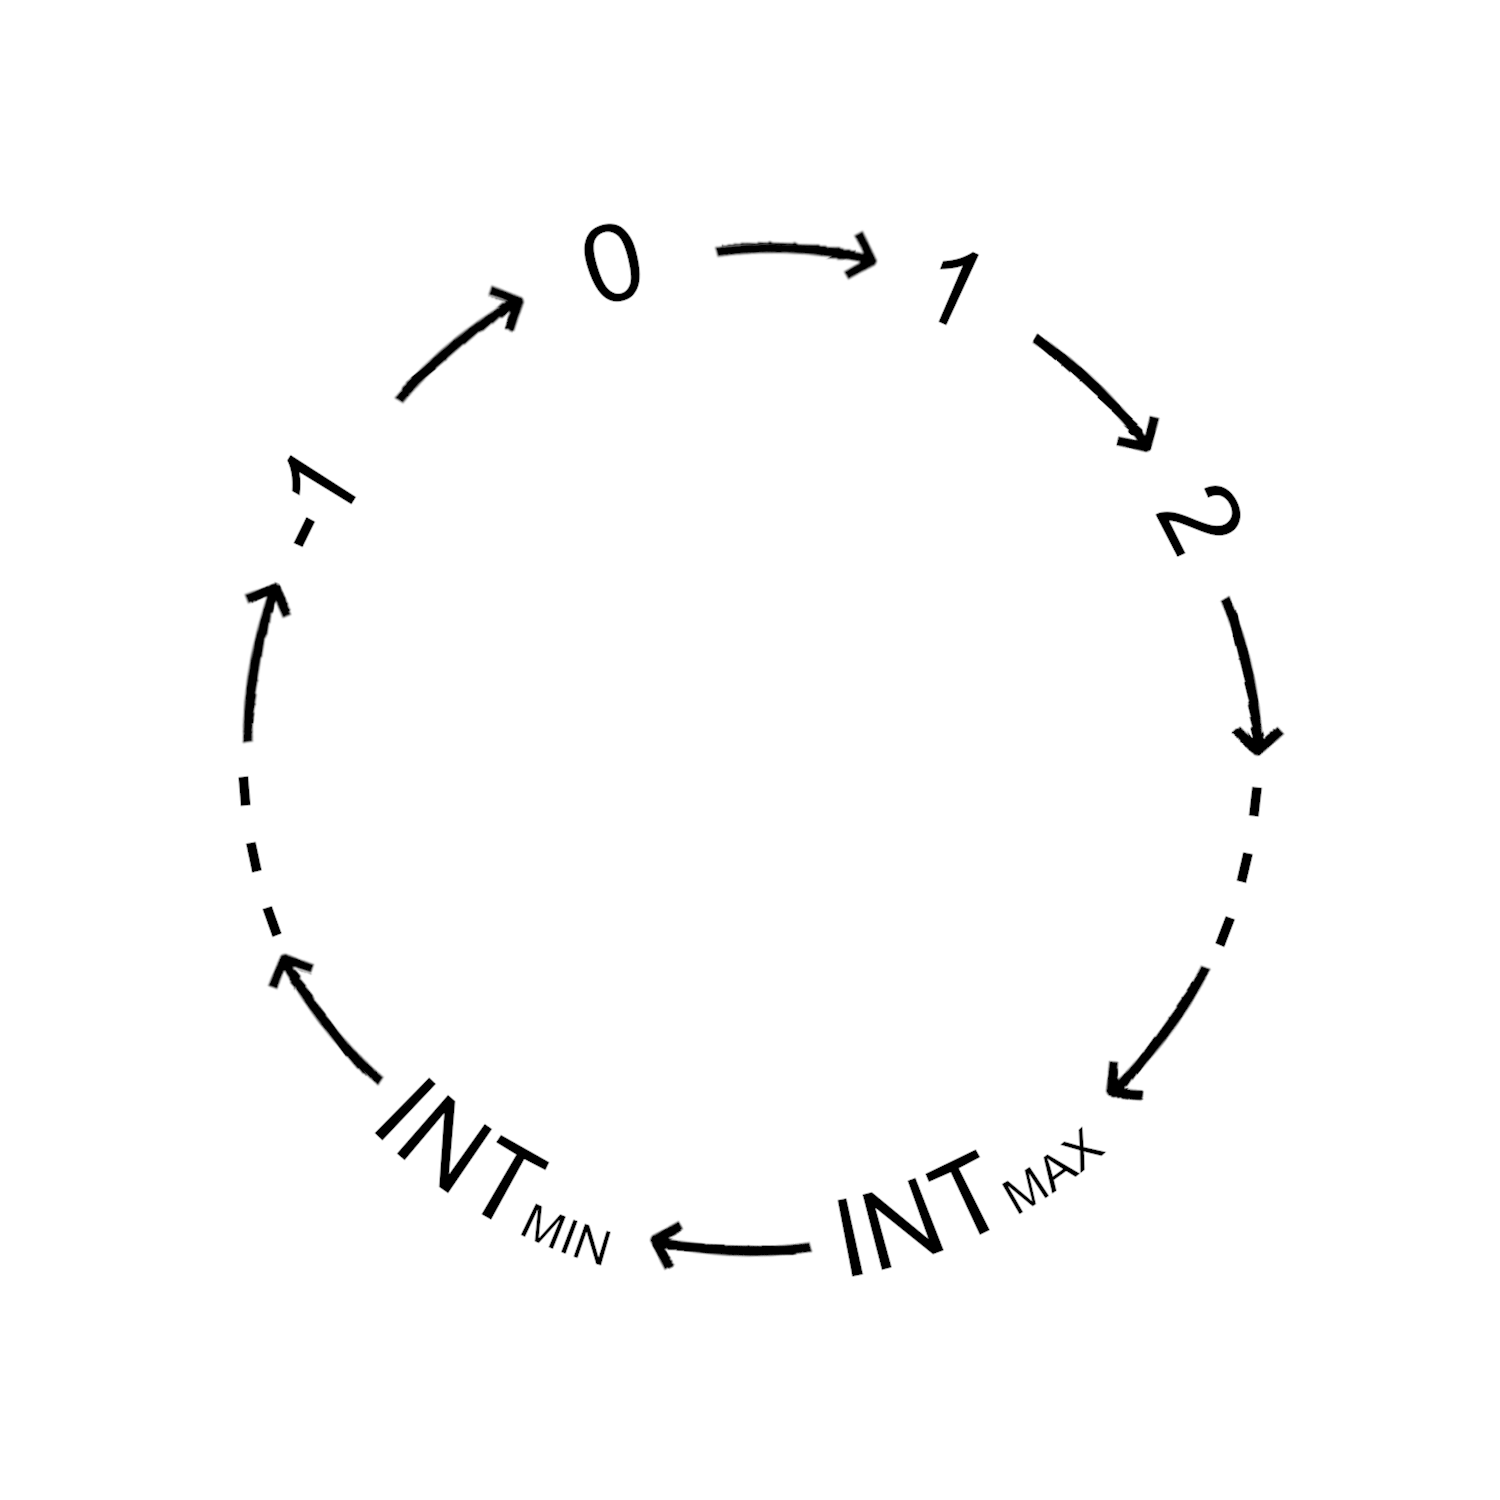
\includegraphics[width=0.5\linewidth]{IntMaxMin.png}}

	\caption{In a computer, integers are arranged like a clock.}\label{fig:INT Rollover}
\end{figure}


	Computers use a binary system instead of a decimal system of representation.\\ \\

\begin{tabbing}
	\hspace*{2cm}\={\textbf{Decimal:}}\hspace*{2cm}\= \hspace*{2cm}\= \hspace*{2cm}\\
	\>$123=1\cdot100+2\cdot10+3\cdot1$\\
	\>$\qquad \! =1\cdot10^2+2\cdot10^1 \! \!+3\cdot10^0$\\ \\
	\>\textbf{Binary:}\\
	\>$_2 1101 = 1\cdot2^3 + 1\cdot2^2+0\cdot2^1+1\cdot2^0$\\ \\
	\>$\qquad \quad \! =1\cdot8 \; +1\cdot4\;\,+0\cdot2 \; +1\cdot1\;=\;_{10}\!13$ \\
\end{tabbing}

\begin{figure}[!htb]
	\center{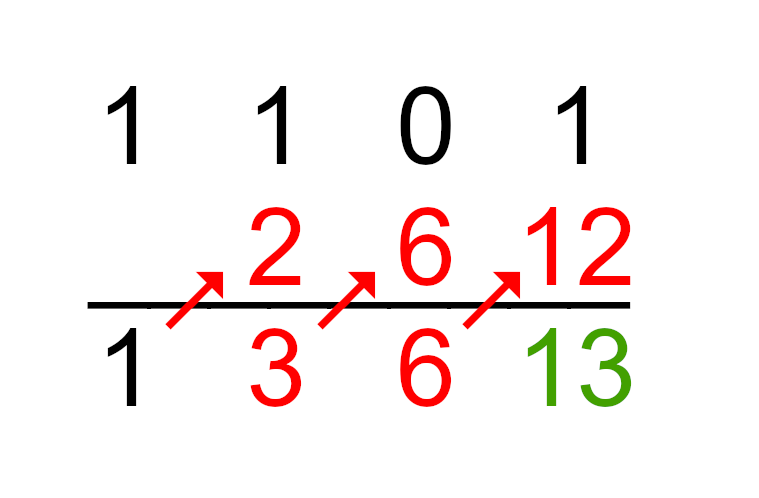
\includegraphics[width=0.5\linewidth]{B2D.png}}
	\caption{One method for binary to decimal conversion is to multiply by 2 and add the next digit.}
	\label{fig:Binary to Decimal Conversion}
\end{figure}

	This scheme corresponds to:

\begin{tabbing}
	\hspace*{2cm}\=$1\cdot2^3+1\cdot2^2+0\cdot2^1+1\cdot2^0$\\
	\>\qquad$=(2^2+1\cdot2^1+0)\cdot2+1$\\
	\>\qquad$=[(1\cdot2+1)\cdot2+0)]\cdot2+1$\\
\end{tabbing}


	How do we go in the other direction?  How does one obtain the binary representation of a decimal 
	integer? Use division with remainders.\\

\begin{figure}[!htb]
	\center{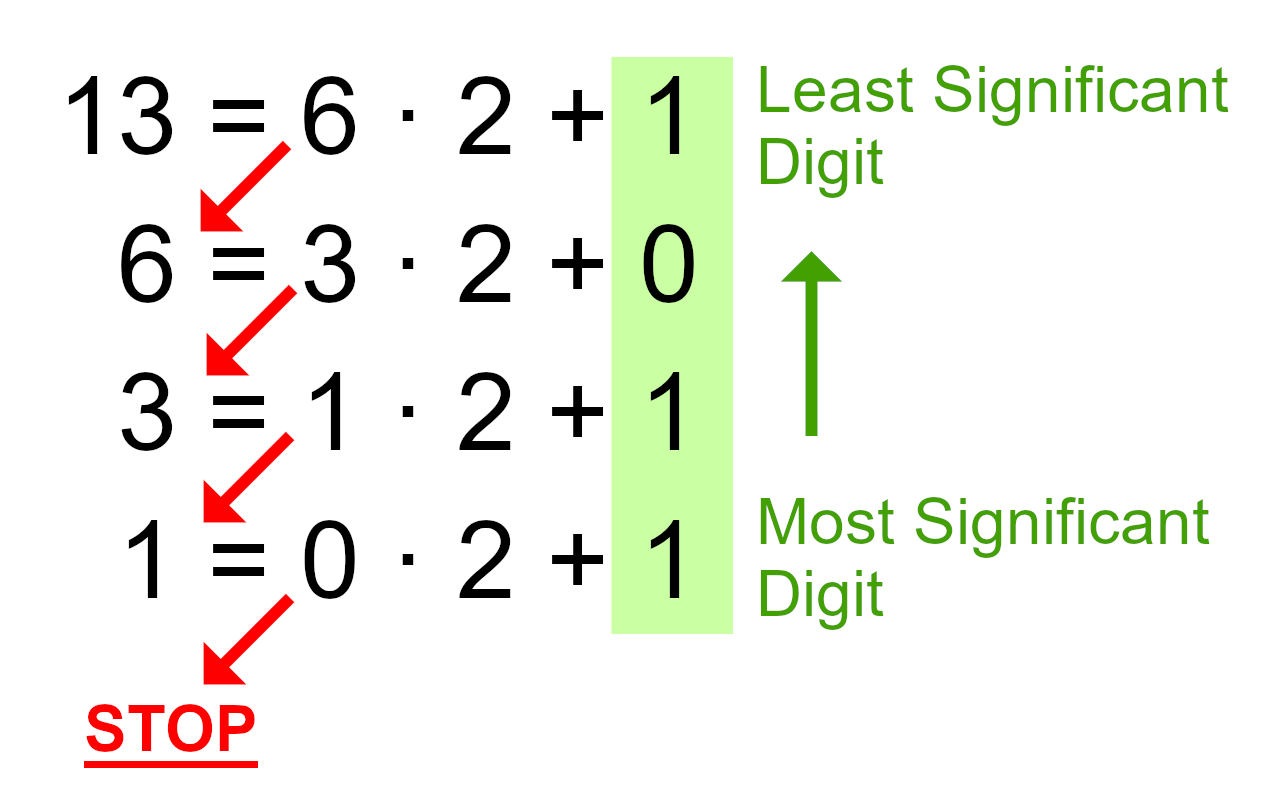
\includegraphics[width=0.5\linewidth]{D2B.png}}
	\label{fig: Decimal to Binary Conversion}
\end{figure}

	For our calculators\\
	$INT_{MAX} = 2147483647$\\ \\
	$INT_{MIN} =-2137483648$\\ \\

	$2147483647 = 1,073,741,824 \cdot 2+1$
	\footnote[3]{The last digit of this number should be 3, but your calculator will round it.} \\[5pt]\\
	$1073741823=536870911\cdot2+1$\\

	$INT_{MAX}=\underbrace{_b111................11}_{\text{31 digits. 1 bit for the sign}}$\\ \\ \\

	If we leave the range $INT_{MAX}, INT_{MIN}$, this is called an \textbf{overflow error}.
	\textit{The computer does not notify us about this!} We have to program all of the necessary 
	checks.

\begin{myindentpar}{1cm}
	\fbox{\parbox{0.85\textwidth}{As long as the computations do not produce an overflow error, 
	arithmetic with
	the datatype INT is \underline{exact}: Addition, subtraction, multiplication, and division with 
	remainders.}}
\end{myindentpar}

\bigskip

	We can extend this to rational numbers:

\begin{center}
	$Rational \; Number=$\large{$\frac{Integer}{Non-Zero\;Integer}$}
\end{center}

	Just store numerator and denominator separately as integers (INTs).\\
	Arithmetic for rational numbers:

\begin{center}
	\Large{$\frac{n_1}{d_1}+\frac{n_2}{d_2}=\frac{n_1d_2+n_2d_1}{d_1d_2}$}
\end{center}

	To avoid unnecessary overflow, cancel the fractions as much and as soon as possible when 
	programming your own routine. For a better interpretation, we can convert
	$\frac{numerator}{denominator}$ into a decimal representation \textit{at the end} of our 
	computations.\\ \\

	\noindent \textbf{Example: \Large{$\frac{13}{12}$}}\\

\begin{center}
	\opdiv[maxdivstep=6]{13}{12}
\end{center}

	The decimal representation will either terminate or will eventually become periodic, as in the 
	preceding example.

% FLOATING POINT NUMBERS -----------------------------------------------------------------------------------
\section{Floating Point Numbers}

	Now let's look at FLOATs. In the sciences and in engineering, we also need very large numbers 
	and very small numbers, i.e close to zero.

\begin{tabbing}
	\hspace*{2cm}\=\textit{Avogadro's Number}\hspace*{2cm}\=$6.022\times10^{23}$\\ \\
	\>\textit{Electrical Charge of}\>$q_e=1.602\times10^{-19}C$\\
	\> \textit{an Elimentary Particle}\\ \\
	\> \textit{Planck's Constant} \>$h=6.626\times10^{-34} m^2kg/s$
\end{tabbing}

	Another number representation is needed. Every real number possesses a decimal representation:

\begin{center}
	$\pm d_k d_{k-1} ... d_0 \underbrace{.}_{\text{\tiny{decimal}}} d_{-1} d_{-2} ....\leftarrow$
	\footnotesize{\textit{May never stop or become periodic}}
\end{center}

	This is a convergent series:

\begin{center}
	$=d_k\cdot10^k+d_{k-1}\cdot10^{k-1}+...+d_0\cdot10^0+d_{-1}\cdot10^{-1}+d_{-2}
		\cdot10^{-2}+...$
\end{center}

	On a computer we can only use finitely many digits.  The number of digits is often called the 
	\textbf{precision}. By moving the decimal point, we standardize these numbers:\\

\begin{center}
\fbox
{
	\parbox{0.5\textwidth}
	{
		\begin{center}
		$\pm \underbrace{d_b.d_{-1}d_{-2}...d_{-p+1}}_{\text{significand}}
			\times10_{\nwarrow_{ Base}}^{k^{\leftarrow Exponent}}$\\
		This is a \textbf{floating point number}.
		\end{center}
	}
}
\end{center}

	It is \textbf{normalized} when there is only one digit, $d_0$ before the decimal point.
	In  other sources, "normalized" is often shown as

\begin{center}
	$\textbf{0}.d_k d_{k-1} ... d_{-3} * 10^{k+1}+ \Delta x$
\end{center}

	For our purposes, a number is normalized when $d_0 \neq 0$, for two main reasons:

\begin{itemize}
	\item This is how FLOATs are stored on computers and calculators.
	\item Scientific Notation (i.e. Avogadro's Constant$\; =6.022 \times 10^{23}$)\\
\end{itemize}

	Also, a computer doesn't use the decimal system.  It uses \textbf{binary}. In binary

\begin{itemize}
	\item base $\; = 2$
	\item digits: 0, 1
\end{itemize}

	In base 2 a normalized floating-point number is

\begin{center}
	$\textbf{1}.b_{-1}b_{-2}...b_{-p+1}*2^E$
\end{center}

	Because the first digit is automatically 1, it is usually not stored in the computer.\\

% RELATIVE ERROR ------------------------------------------------------------------------------------------------
\section{Relative Error}
	To get a feeling for floating point numbers, let's study a very limited "Toy" number system:
	 $1.b_{-1} b_{-2}\cdot2^E$

\begin{center}
	\begin{tabular}{c|c?c?l}
		$b_{-1}$&$b_{-2}$&\footnotesize{E}&\footnotesize{Decimal Value}\\
		\hline
		0&0&0&$1+0\cdot\frac{1}{2}+0\cdot\frac{1}{4}=1$\\
		0&1&0&$1+0\cdot\frac{1}{2}+1\cdot\frac{1}{4}=1.25$\\
		1&0&0&$1+1\cdot\frac{1}{2}+0\cdot\frac{1}{4}=1.5$\\
		1&1&0&$1+1\cdot\frac{1}{2}+1\cdot\frac{1}{4}=1.75$\\
		\hline
		0&0&1&$\quad \; 1\cdot2^1=2$\\
		0&1&1&$1.25\cdot2^1=2.5$\\
		1&0&1&$\; \,1.5\cdot2^1=3$\\
		1&1&1&$1.75\cdot2^1=3.5$\\
	\end{tabular}
\end{center}

%\pagebreak

\begin{center}
	\begin{tabular}{c|c|c?r|r|r|r}
		1.&$b_{-1}$&$b_{-2}$&\footnotesize{$E=-1$}&\footnotesize{$E=0$}&\footnotesize{$E=1$}
		&\footnotesize{$E=2$}\\
		\hline
		&0&0&0.5&1&2&4\\
		&0&1&0.625&1.25&2.5&5\\
		&1&0&0.75&1.5&3&6\\
		&1&1&0.875&1.75&3.5&7\\		
	\end{tabular}
\end{center}

\bigskip
\bigskip
\bigskip

\begin{footnotesize}
\begin{center}
	\begin{tikzpicture}
    		\begin{tikzpicture}
        			\begin{axis}
				[
            			% center the x axis
            			axis x line=middle,
            			% we don't need a y axis line ...
            			axis y line=none,
            			% ... and thus there is no need for much `height' of the axis
            			height=50pt,
            			% but `height' also changes `width' which is restored here
            			width=\textwidth,
            			xmin=-0.5,
           		 	xmax=7.5,
				xtick={0,1,...,7},
				extra x ticks = {0.5, 1.5,...,6.5},
				extra x tick labels={},
        				]
            			\addplot+[only marks, mark=otimes*, color=blue]
					coordinates {(0.5,0) (0.625,0) (0.75,0) (0.875,0)};
 	 			\addplot+[only marks, mark=otimes*, color=violet]
					coordinates{(1,0)(1.25,0)(1.5,0)(1.75,0)};
				\addplot+[only marks, mark=otimes*, color=orange]
					coordinates {(2,0) (2.5,0) (3,0) (3.5,0)};
				\addplot+[only marks, mark=otimes*, color=red]
					coordinates {(4,0) (5,0) (6,0) (7,0) };
 				\path (0.5,0) coordinate (A1)
					(0.875,0) coordinate (A2)
					(1,0) coordinate (B1)
					(1.75,0) coordinate (B2)
					(2,0) coordinate (C1)
					(3.5,0) coordinate (C2)
					(4,0) coordinate (D1)
					(7,0) coordinate (D2);      
    			\end{axis}
 			\draw[decorate,decoration={brace,raise=2.5em}]
				(A2) -- (A1) node[midway,below=2.6em]
				{$_{E=-1}$};
			\draw[decorate,decoration={brace,raise=2.5em}]
				(B2) -- (B1) node[midway,below=2.6em] {$E=0$};
			\draw[decorate,decoration={brace,raise=2.5em}]
				(C2) -- (C1) node[midway,below=2.6em] {$E=1$};
			\draw[decorate,decoration={brace,raise=2.5em}]
				(D2) -- (D1) node[midway,below=2.6em] {$E=2$};
    		\end{tikzpicture}
	\end{tikzpicture}
\end{center}
\end{footnotesize}

	Note that the distance between the numbers depends on their size. Consequentially, the round off 
	error will also be affected by the size of the number. For this reason it's important to use 
	\textit{relative error} instead of absolute error.\\

\begin{tabbing}
	\hspace*{2cm}\=Absolute Error \hspace*{1cm} \= $x+ \Delta x$ \\
	\> Relative Error \> $x(1+ \frac{\Delta x}{x})=x(1+ \delta x)$\\
\end{tabbing}

	Often the relative error is the better way to measure the round off error of floating point numbers.

\begin{center}
	$fl(x)=x(1+ \delta x) \Leftrightarrow \delta x = \frac{fl(x)-x}{x}$
\end{center}

% RELATIVE ERROR EXAMPLE ------------------------------------------------------------------------------------
\section{Relative Error Examples}

	\textbf{Example 1:} Real number, 4 digits, base 10:

\begin{tabbing}
	\hspace{3cm}\=$\quad \; \; x= \underbrace{1.234}_{\tiny{4digits}}\!56$\\
	\> \\
	\>$fl(x)=1.235$\\
	\> \\
	\>\large{$\quad \!  \delta x = \frac{1.235-1.23456}{1.23456}$}\\
	\> \\
	\>$\qquad \; \; = \frac{0.00044}{1.23456}=0.000356$\\
	\> \\
	\> $\qquad \; \; \simeq 0.0004 \; \leftarrow$ \footnotesize{Only first non-zero digit}
\end{tabbing}

	For errors, only record record the first non-zero (in most cases). When the first non-zero digit is 1, 
	record the next digit (which can be zero).\\ \\

	\noindent \textbf{Example 2:} $y=123.456 = 1.23456 \times 10^2$

\begin{tabbing}
	\hspace{3.5cm}\=$fl(y)=1.235 \times 10^2$\\
	\> \\
	\> \quad \large{$\delta y = \frac{1.235 \times 10^2-1.23456 \times 10^2}{1.23456 \times 10^2}$}\\
	\> \\
	\> \qquad \; \large{$= \frac{0.00044 \times 10^2}{1.23456 \times 10^2}\, ^{\leftarrow Absolute \; Error}$}\\
	\> \\
	\> \qquad \; $\simeq 0.0004{\leftarrow Relative \; Error}$
\end{tabbing}

	Notice how the relative error size reflects the number of digits used in the system. If a decimal 
	system uses $k$ digits, then the relative round-off error is bounded by $5 \times 10^{-k}$.\\

% SPECIAL FLOATS -------------------------------------------------------------------------------------------------

\section{Subnormal Numbers and other special FLOAT values}

	Note in the number line from earlier that there is a gap at zero.  What do we do about this gap?  
	How do we express zero itself as a FLOAT? Not only is the number of digits in the mantissa finite, 
	but the number of digits in the exponent is also finite. In C and other programming languages 
	FLOATs are 32 Bits.  23 of these bits are used for the significand, 7 for the exponent, and 1 for the 
	sign.\\ \\

	In our toy system from earlier, let's use $-2\leq  E \leq 4$
	
\begin{tabbing}
	\hspace*{2cm}\= \textit{Use the maximal exponent for} \\
	\hspace*{3cm}\=INF \hspace*{1cm} \=  infinity (overflow error)\\
	\> NaN \> "not a number"
\end{tabbing}

	These two are distinguished by using different mantissae.

\begin{tabbing}
	\hspace*{2cm}\= \textit{Use the minimal exponent for \textbf{subnormal numbers:}}
		$\textbf{0}.b_{-1}b_{-2}\times 2^{-2}$ \\
	\hspace*{3cm}\=$0.00\times 2^{-2}$ \hspace*{1cm} \=  0\\
	\>$0.01\times 2^{-2}$ \>$\frac{1}{8}$\\
	\>$0.10\times 2^{-2}$ \>$\frac{1}{4}$\\
	\>$0.11\times 2^{-2}$ \>$\frac{3}{8}$\\
\end{tabbing}

	What is the relative error in our toy system?

\begin{center}
	$\frac{1}{8}=2^{-3}=\frac{1}{2} \times 2^{-2}$
\end{center}

% Notes are a bit spotty here -------------------------------------------------------------------------------------
	Go to seven, which in binary is

\begin{center}
	$1.11 \times 2^2$\\
	$\frac{1}{8} \times 2^2$\\
\end{center}

% --------------------------------------------------------------------------------------------------------------------

	Some example of relative errors in our binary toy system:

\begin{center}
	$\frac{7-7.4}{7.4}\simeq -0.05$\\
	\bigskip
	$\frac{7-6.6}{6.6} \simeq 0.06$\\
	\bigskip
	$\frac{8-8.9}{8.9} \simeq -0.10$\\
\end{center}

	Why are subnormal numbers treated differently?

\begin{center}
	\begin{Large}
	$\frac{fl(\frac{1}{16})-\frac{1}{16}}{\frac{1}{16}}
		=\frac{\frac{1}{8}-\frac{1}{16}}{\frac{1}{16}}
		=\frac{\frac{2}{16}-\frac{1}{16}}{\frac{1}{16}}=\frac{\frac{1}{16}}{\frac{1}{16}}=1$
	\end{Large}
\end{center}

	Relative error $2^{-3}$ does not hold for sub-normal numbers, only normalized numbers.  
	Because of this, it is of the utmost importance to \textit{\textbf{avoid dividing by numbers close to 
	zero whenever possible!}}

% ADDING FLOATS ------------------------------------------------------------------------------------------------
\section{Adding FLOATs}

	Now we know the general shape of the machine number system FLOAT, how does arithmetic work 
	with it?

\begin{center}
	Toy System: $\Bigg( \bigg( \Big( \left(4\oplus \frac{1}{4}\right) \oplus \frac{1}{4}\Big)
		\oplus \frac{1}{4}\bigg) \oplus \frac{1}{4}\Bigg)=4$
\end{center}

	The sum of two machine numbers may not be a machine number.  Addition my create more round-
	off errors.

\begin{tabbing}
	\hspace*{4cm}\= $\qquad 4 \oplus \bigg(\frac{1}{4}\oplus\Big( \frac{1}{4}\oplus\left(\frac{1}{4}\oplus \frac{1}{4}\right)\Big)\bigg)$\\
	\> \\
	\>$ \quad=4 \oplus \Big( \frac{1}{4} \oplus\left( \frac{1}{4} \oplus \frac{1}{2}\right)\Big)$\\
	\> \\
	\>$ \quad=4 \oplus \left( \frac{1}{4} \oplus \frac{3}{4}\right) = 4 +1 = 5$\\
\end{tabbing}

	If you must add lots of numbers on a computer, add them in order from small to large, to minimize 
	round-off error.\\

	\noindent \textbf{Example:} Harmonic Series

\begin{center}
	$1+\frac{1}{2}+\frac{1}{3}+\frac{1}{4}+\frac{1}{5}+\frac{1}{6}+...$
\end{center}

\begin{itemize}
	\item{Divergent Series}
	\item{Partial sums "approach" infinity.}
\end{itemize}

	We try to recreate the harmonic series in a C program:

\begin{center}
\fbox
{
	\parbox{0.5\textwidth}
	{
		\texttt{
			\begin{tabbing}		
				\hspace*{0.7cm}\=float sum;\\
				\>sum = 0.0;\\
				\>for (i=1; i<= 1\,000\,000; i++)\{\\
				\>\qquad sum += 1/(float) i;\\
				\>\}\\
			\end{tabbing}}
	}
}
\end{center}

	We repeat this same for-loop, increasing the size of the loop from \texttt{i<=1\,000\,000} to 
	10,000,000 and 100,000,000.  The program returns the following results:
\begin{center}
\fbox
{
	\parbox{0.5\textwidth}
	{
		\texttt{
			\begin{tabbing}		
				\hspace*{0.5cm}\=1\,000\,000 summands give sum 14.3573579788\\
				\>10\,000\,000 summands give sum 15.4036827087\\
				\>100\,000\,000 summands give sum 15.4036827087
			\end{tabbing}}
	}
}
\end{center}

	We see that by adding increasingly smaller summands the computer has already run out of 
	precision before 10,000,000 cycles.  If we reverse the order of the for-loop so that the script adds 
	summands in ascending order from smallest to largest we obtain the following results:

\begin{center}
\fbox
{
	\parbox{0.5\textwidth}
	{
		\texttt{
			\begin{tabbing}		
				\hspace*{0.5cm}\=1\,000\,000 summands give sum 14.3926515579\\
					\>10\,000\,000 summands give sum 16.6860313416\\
					\>100\,000\,000 summands give sum 18.8079185486\\
					\>1\,000\,000\,000 summands give sum 18.8079185486
			\end{tabbing}}
	}
}
\end{center}

	By adding the summands from smallest to largest, it takes the script is able to add smaller numbers, 
	and so obtain a larger partial sum.  \textit{When programming, if possible try to add smaller 
	numbers first, for more accurate results.}


\pagebreak
% CONFER WITH PROFESSOR KEHREIN ABOUT THIS BIT! ----------------------------------------------------
%-------------------------------------------------------------------------------------------------------------------------
\begin{tabbing}
	\hspace*{2cm}\=$0.1 =
		\underbrace{ b_{-1}}_{=0}\frac{1}{2}+b_{-2}\frac{1}{2^2}+b_{-3}\frac{1}{2^3}+...$\\
	\footnotesize{Multiply by 2:}\\
	\>$0.2 = \underbrace{b_{-1}}_{=0}+b_{-2}\frac{1}{2}+b_{-3}\frac{1}{2^2}+...$\\
	\footnotesize{$\times 2:$}\\
	\>$0.4 =b_{-2}+b_{-3}\frac{1}{2}+b_{-4}\frac{1}{2^2}+...$\\
	\footnotesize{$\times 2:$}\\
	\>$0.8 =b_{-3}+b_{-4}\frac{1}{2}$
\end{tabbing}
%------------------------------------------------------------------------------------------------------------------------
%------------------------------------------------------------------------------------------------------------------------

	A particular C program adds \texttt{float 0.0 += 0.1}, with the following results:

\begin{tabbing}
	\hspace*{2cm}\=$fl(0.1)=0\,.\,100\,000\,001\,5$\\
	\>$fl(0.2)=0\,.\,200\,000\,003\,0$\\
	\>$fl(0.3)=0\,.\,300\,000\,011\,9$\\
	\>$fl(0.4)=0\,.\,400\,000\,006\,0$\\
	\>$fl(0.5)=0\,.\,500\,000\,000\,0$\\
	\>$fl(0.6)=0\,.\,600\,000\,023\,8$\\
	\>$fl(0.7)=0\,.\,700\,000\,047\,7$\\
	\>$fl(0.8)=0\,.\,800\,000\,071\,5$\\
	\>$fl(0.9)=0\,.\,900\,000\,095\,4$\\
	\>$fl(1.0)=0\,.\,200\,000\,119\,2$\\
\end{tabbing}

\begin{center}
	\begin{tabular}{r?c|l}
	$b_0$ & \textbf{0} & \textbf{.1}$\leftarrow$ \textit{Double the fractional part}\\
	$b_{-1}$ & 0 &.2\\
	$b_{-2}$ &0 &.4\\
	$b_{-3}$ &0 &.8\\
	\textit{Discard whole part} $\rightarrow$&1 &.6\\
	$b_{-5}$ &1 &.2 $\leftarrow$\textit{Numbers repeat}\\
	$b_{-6}$ &0 &.4\\
	\end{tabular}
\end{center}

	The whole part becomes the binary representation, hence:

\begin{center}
	$fl(_{10}0.1) = \underbrace{_20}_{b_0}\! \! \!.000\,110\,011\,001\,1...
		 = _2\!0.000\,\overline{1100} $\\
	$=\underbrace{_2 1.\;1}_{\text{Normalized}}\!\!\!\!\!001\;1001\;1001 ... \times 2^{-4}$\\
\end{center}

	FLOATs use 23 fractional bits, so this non-terminating number will be rounded:

\begin{center}
	$fl(_{10}0.1)=1.1001\;1001\;1001\;1001\;1001\;10\cancelto{1}{01}\times 2^{-4}$
\end{center}

	Let's compute the round-off error:

\begin{tabbing}
	\hspace*{2cm}\=\footnotesize{absolute error$\rightarrow$} \hspace*{0.25cm}\=$\Delta x
		=1\times2^{-23}\times2^{-4}-1.1001\;1001\;...\times2^{-24}\times2^{-24}$\\
	\>\> $\qquad \! \!= 2^{-3}\times2^{-24}-_{10}0.1\times2^{-24}$\\
	\>\> $\qquad \! \!= (_{10}0.125-_{10}0.1)\times2^{-24}$\\
	\>\> $\qquad \! \!=_{10}\!1.49\times10^{-9}\simeq1.5\times10^{-9}$\\

\end{tabbing}

	Now let's add two FLOAT values:

\begin{center}
	\begin{tabular}{rrccccccr}
		& \tiny{$1\;1\;\;$} &  \tiny{$\quad\, \;1\;1$} & \tiny{$\quad\, \;1\;1$} 
			& \tiny{$\quad\, \;1\;1$} & \tiny{$\quad\, \;1\;1$} & \tiny{$\quad\, \;1\;1$} 
			& \tiny{$1$} & \\
		$fl(0.1)=$ & $1.$ & $\!1001$ & $1001$ & $1001$ & $1001$ & $1001$ & $101$ 
			& $\times2^{-4}$\\
		$+\;fl(0.1)=$ & $+1.$ & $\!1001$ & $1001$ & $1001$ & $1001$ & $1001$ & $101$ 
			& $\times2^{-4}$\\
		\hline
		$_{\text{Not normalized}}\rightarrow$& $11.$ & $\!0011$ & $0011$ & $0011$ & $0011$ 
			& $0011$ & $010$ & $\times2^{-4}$\\ \\
	\end{tabular}

	$fl(0.2) = 1.\;1001\;1001\;1001\;1001\;1001\;101\cancelto{round-off}{0} \times2^{-3}$
\end{center}

	To add an additional $fl(0.1)=1.100...\times2^{-4}$ we have to shift the mantissa to adjust the 
	exponent.

\begin{center}
	\begin{tabular}{rrccccccr}
		&\tiny{$1\;1\;\;$} & \tiny{$\quad\, \;1\;1$} & \tiny{$\quad\, \;1\;1$}
			& \tiny{$\quad\, \;1\;1$} & \tiny{$\quad\, \;1\;1$} & \tiny{$\quad\, \;1\;1$}
			& \tiny{$1\;1\quad \;\,$} & \\
		$fl(0.2)=$ & $1.$ & $\!1001$ & $1001$ & $1001$ & $1001$ & $1001$ & $101\;\,$ 
			& $\times2^{-3}$\\
		$+\;fl(0.1)=$ & $+\;0.$ & $\!1100$ & $1100$ & $1100$ & $1100$ & $1100$ 
			& $11\cancelto{1}{0}\cancel{1}$ & $\times2^{-3}$\\
		\hline
		$_{\text{Normalize}}\rightarrow$& $10.$ & $\!0110$ & $0110$ & $0110$ & $0110$ 
			& $0110$ & $100$ & $\times2^{-3}$\\ \\

		$\Rightarrow$ & $1.$ & $\!0011$ & $0011$ & $0011$ & $0011$ & $0011$ & $010$ 
			& $\times2^{-2}$\\ \\
	\end{tabular}
\end{center}

	Is this floating point number representative of $_{10}0.3$? Let's check!

\begin{center}
	\begin{tabular}{r|l}
	\textbf{0} & \textbf{.3}\\
	0 &.6\\
	1 &.2\\
	0 &.4\\
	0 &.8\\
	1 &.6 $\leftarrow Numbers\; repeat$\\
	$Repeating\; pattern: 0011\! \rightarrow$1 &.2 \\
	\end{tabular}
\end{center}

% Section requires computer data (Xcel) --------------------------------------------------------------------------
	To add $fl(0.1)$ at this point, we must adjust the exponent by two.  There are two options: First, we can shift 
	by one digit twice, which would lead to two 	cases of rounding up. The second option is to shift by two digits at 
	once, which leads to rounding down.  Looking at the results from the computer, we see that the second method 
	is chosen.
%------------------------------------------------------------------------------------------------------------------------

\begin{center}
	\begin{tabular}{rccccccr}
		&  \tiny{$1\;1\qquad\!$} & \tiny{$1\;1\qquad\!$} &  \tiny{$1\;1\qquad\!$} 
			& \tiny{$1\;1\qquad\!$} & \tiny{$1\;1\qquad\!$} & \tiny{$1\qquad \!$} & \\
		$1.$ & $\!0011$ & $0011$ & $0011$ & $0011$ & $0011$ & $010$ & $\times2^{-2}$\\
		$+\;0.$ & $\!0110$ & $0110$ & $0110$ & $0110$ & $0110$ & $011$ & $\times2^{-2}$\\
		\hline
		$1.$ & $\!1001$ & $1001$ & $1001$ & $1001$ & $1001$ & $101$ & $\times2^{-2}$\\
		&&&&&&$\;\;=$& $\! \! \! \!fl(0.4)$\\ \\
	\end{tabular}

	\bigskip

	\begin{tabular}{rrccccccr}
		&\tiny{$1\;1\;\;$} &  \tiny{$1\;1\;1\;1$} & \tiny{$1\;1\;1\;1$} &  \tiny{$1\;1\;1\;1$} 
			& \tiny{$1\;1\;1\;1$}& \tiny{$1\;1\;1\;1$} & \tiny{$1\;1\quad \;\,$} & \\
		$fl(0.4)=$ & $1.$ & $\!1001$ & $1001$ & $1001$ & $1001$ & $1001$ & $101$
			& $\times2^{-2}$\\
		$+\;fl(0.1)=$ & $\!+\;0.$ & $\!0110$ & $0110$ & $0110$ & $0110$ & $0110$ & $011$ 
			& $\times2^{-2}$\\
		\hline
		$_{\text{Normalize}}\rightarrow$& $10.$ & $\!0000$ & $0000$ & $0000$ & $0000$ 
			& $0000$ & $000$ & $\times2^{-2}$\\ \\

		$fl(0.5)=$ & $1.$ & $\!0000$ & $0000$ & $0000$ & $0000$ & $0000$ & $000$ 
			& $\times2^{-1}$\\ \\
	\end{tabular}
\end{center}

	\textbf{Note:} In this program $fl(0.5)= 0.5$

\begin{center}
\fbox
{
	\parbox{0.5\textwidth}
	{
			\textbf{\underline{Side Remark:}} When programming FLOAT results, allow for round-off 
			errors. Don't use conditions like
			\begin{center}
				\texttt{result == 0.0}
			\end{center}
			Instead use
			\begin{center}
				\texttt{result $<$= 0.00....1}
			\end{center}
			Don't use values that are \underline{too} small, though.
	}
}
\end{center}

	One more step:\\
\begin{center}
	\begin{tabular}{rrccccccl}
		$fl(0.5)=$ & $1.$ & $\!0000$ & $0000$ & $0000$ & $0000$ & $0000$ & $\!\!\!000$
			& $\times2^{-1}$\\
		$+\;fl(0.1)=$ & $\!+\;0.$ & $\!0011$ & $0011$ & $0011$ & $0011$ & $0011$
			& $0\!\!\!\underbrace{10}$ & $\times2^{-1}$\\
		&&&&&&& $\;\;\;\;\nwarrow$ &$_{\!\!\!\!\!\!\!\text{two digits affected}}$\\
		\hline
		& $1.$ & $\!0011$ & $0011$ & $0011$ & $0011$ & $0011$ & $\!\!\!010$
			& $\times2^{-1}$\\ \\

	\end{tabular}
\end{center}

	Because $fl(0.1)$ needs to be rounded by two digits, there is a larger error in this operation.
	\textbf{Shifting loses significant digits!}  Many other math texts ignore this effect.\\ \\

	We may think that the round-off error is gone at 0.5 because it can be represented \textit{exactly}
	by a machine number, but notice that 1 is also a machine number, and we have a huge round-off 
	error there.\\ \\

	So far we've had
\begin{center}
	\begin{tabular}{rl}
		& $fl(0.x)+fl(0.1)=fl(0.x+1)$\\
		& \\
		\textit{i.e.}& $fl(0.4)+fl(0.1)=fl(0.5)\qquad$\\
		& \\
		& \\
		\textit{Note that:}& \\
		& $\underbrace{fl(0.9)+fl(0.1)}_{_{\text{severe round-off error}}} \neq fl(1.0)$\\
		& \\
		\textit{Since} & $fl(1.0) = 1.0$.
\end{tabular}
\end{center}

	Where does this happen the first time and why?  Notice in the preceding example we do not have a 
	simple case of error propagation. The roundoff error of $fl(0.1)$ does not simply accumulate in the 	
	sum. \\

	What errors are produced by arithmetic operations?  Sometimes a sum, difference, product, or 
	quotient of machine numbers is not a machine number. So there are round-off errors produced by 
	arithmetic, not just number representation. (Other texts provide rather limited information about 
	this.) Additionally, how do errors propagate if we begin with uncertain numbers (i.e. measurement 
	data). \\

% Finding Zeros of Functions --------------------------------------------------------------------------------------
\section{Finding Zeros of Functions}

	How do we compute function values? Due to round-off errors, can we really detect zeros? If a 
	function gets very close to zero, how can we determine whether its value is really different from 
	zero, or just a zero with a round-off error?\\

	\noindent \textbf{Example:}\medskip\\
	
	\noindent In our toy system with normalized floating-point numbers, of the form 
	$b_0.b_{-1}b_{-2}\times 2^E$ we found:

\begin{center}
	$4\oplus \frac{1}{4} = 4$\\
	\bigskip
\end{center}

	Why?

\begin{center}
	$fl(4)=_2 1.00\times 2^2$\\
	\medskip
	$\; \; fl(\frac{1}{4})=_2 1.00\times 2^{-2}$
\end{center}

	Add them:

\begin{center}
	\textit{Shift the $fl(\frac{1}{4})$ to adjust the exponent:}\\
	\medskip
\begin{tabular}{rcll}
	$fl_{shifted}(\frac{1}{4})\;=$ & $\!\!0.00$ & $\!\!\!\!\cancelto{\text{round down}}{01}$ & $\times 2^2$\\
	$+ \; fl(4)\;=$ & $\!\!1.00$ & & $\times 2^2$\\
	\hline
	& $\!\!1.00$ & & $\times 2^2 \; = fl(4)$\\
\end{tabular}
\end{center}
	\bigskip

	What size of error do we get here?

\begin{center}
	\large{$\delta_{sum}=\frac{4-4.25}{4.25}=\frac{-0.25}{4.25}\simeq -0.06$}
\end{center}

	\medskip
	Upper bound for relative error: $_2 0.001 = _{10}0.125$\\

	Notice, however, that we can make the error arbitrarily large by repeated addition:

\begin{center}
	$\bigg(\Big(\left(4 \oplus \frac{1}{4}\right)\oplus \frac{1}{4}\Big)\oplus \frac{1}{4}\bigg)\oplus \frac{1}{4}$\\
	\medskip
	\large{$\delta =$ \Large{$\frac{4-5}{5}$}$\,=\,$\Large{$\frac{-1}{5}$}$\,=-0.2$}\\
\end{center}
	\medskip

	We have already seen that adding smaller summands first improves the accuracy.

% FLOAT MULTIPLICATION ---------------------------------------------------------------------------------------
\section{FLOAT multiplication}

	\noindent \textbf{Example:} Use decimal system with three digits:

\begin{tabbing}
	\hspace*{5cm} \=$(1.23 \times 10^4)\cdot(4.56 \times 10^3)$\\
	\> $\;=5.6088 \times 10^7$\\
	\> $\Rightarrow 5.61 \times 10^7$
\end{tabbing}

	Rounding is necessary, but within the rounding bounds of the number system.  For multiplication, 
	the error propagation can be described rather easily:

\begin{tabbing}
	\hspace*{5cm}\= $[x(1+\delta x)]\cdot[y(1+\delta y)]$\\
	\>$= (x+x\cdot\delta x)(y+y\cdot\delta y)$\\
	\>$= xy + xy\delta x + xy\delta y + xy \delta x \delta y$\\
	\> $= xy(1 + \delta x + \delta y + \!\!\!\underbrace{\delta x \delta y}_{negligible}\!\!\!)$\\
	\> $\simeq xy(1+ \delta x + \delta y)$
\end{tabbing}

	The relative error of the product is (to a very good approximation) the sum of the relative errors of 
	the factors. The relative errors don't explode.  They grow slowly.

% FLOAT DIVISION -------------------------------------------------------------------------------------------------
\section{FLOAT Division}

	\noindent \textbf{Example:} Use decimal system with three digits:

\begin{tabbing}
	\hspace*{4cm}\=\Large{$\frac{1.23 \times 10^4}{4.56 \times 10^3}$}
	\hspace*{0.1cm}\=\normalsize{$=0.2697\times 10^1$}\\
	\>\>$=2.697\times 10^0 \!\leftarrow$\footnotesize{\textit{Write exponent so it isn't forgotten!}}\\
	\> \> $\Rightarrow 2.70 \times 10^0$\\
	\> \Large{$\frac{x(1+\delta x)}{y(1+\delta y)}$}\>=\Large{$\frac{x}{y}$}
		\normalsize{$(1+\delta x)
		(\underbrace{1-\delta y+(\delta y)^2-(\delta y)^3+-...}_{\text{Geometric series.}\;\delta y\;
		\text{can be assumed}\;<1})$}
\end{tabbing}

\begin{center}
\fbox
{
	\parbox{0.6\textwidth}
	{
			\textbf{\underline{Geometric Series}:}
			\begin{center}
				$1+ (-\delta y) + (-\delta y)^2 + (-\delta y)^3 + ...
				=$ \large{$\frac{1}{1-(-\delta y)}$}\\
				\medskip
				for $\left| \delta y \right| <1$
			\end{center}
	}
}
\end{center}

\begin{tabbing}
	\hspace*{4.1cm}\=\Large{$\frac{x(1+\delta x)}{y(1+\delta y)}$}
	\hspace*{0.1cm} \= \normalsize{$=$} \Large{$\frac{x}{y}$}
		\normalsize{$(1 + \delta x - \delta y + \text{\small{\textit{[smaller terms]}}})$}\\
	\medskip \\
	 \>\> \normalsize{$\simeq$} \Large{$\frac{x}{y}$} \normalsize{$1+ \delta x - \delta y$}
\end{tabbing}

	As with multiplication, the relative errors in division can add up but can also partially cancel each 
	other out. \textit{Multiplication and Division behave nicely }for FLOATS.


% FLOAT SUBTRACTION------------------------------------------------------------------------------------------------------------------------
\section{FLOAT Subtraction}

	Subtraction is very problematic when values are \textit{almost}  equal.

\begin{tabbing}
	\hspace{3cm}\= $4.56 \times 10^3 - 4.55 \times 10^3$
	\hspace{0.1cm}\=$ = \!\!\!\!\!\!\!\!\!\!\!\!\!\!\!\!\!\!\underbrace{0.0}_{\text{Two significant digits 
	lost!}} \!\!\!\!\!\!\!\!\!\!\!\!\!\!\!\!\!\!\!\!\!\! 1 \times 10^3$\\ \\
	Normalize: \>\>$=1.\!\!\!\!\!\!\!\!\!\!\!\!\!\!\!\!\!\!\!\!\!\!\!\!\!\!\!\!\!\!
		\underbrace{00}_{\text{These could be 9. We don't know!}}
		\!\!\!\!\!\!\!\!\!\!\!\!\!\!\!\!\!\!\!\!\!\!\!\!\!\!\!\!\! \times 10^1$
\end{tabbing}
	
	Such results are usually \textit{very} uncertain. \textit{Avoid formulas that lead to differences of 
	almost equal numbers!}\\ \\

	\noindent \textbf{Example 1:}

\begin{tabbing}
	\hspace*{4cm} \= $\ln5000-\ln4999$ \hspace*{0.1cm}\= $\simeq 8.51719391 - 8.516993171$\\
	\> \> $\simeq 2.0002 \times10^{-4}$ \\
	Alternatively:\\
	\> $\qquad \qquad \; \ln$ \Large{$\!\frac{5000}{4999}$}\> $\simeq 2.000199947
		\times 10^{-4}$
\end{tabbing}

	\noindent \textbf{Example 2:}

\begin{tabbing}
	\hspace*{4cm} \= $f(t)$ \hspace*{0.1cm} \= $\!\! =$ \Large{$\frac{\sqrt{t^2+9}-3}{t^2}$}\\ \\
	This equation can be rewritten:\\
	\> \>$\!\! =$ \Large{$\frac{\sqrt{t^2+9}-3}{t^2} \cdot
		\frac{\sqrt{t^2+9}+3}{\sqrt{t^2+9}+3}$}\\ \\
	\> \> $\!\! =$ \Large{$\frac{t^2+9-9}{t^2(\sqrt{t^2+9}+3)}$}\\ \\
	\> \> $\!\! =$ \Large{$\frac{1}{\sqrt{t^2+9}+3}$}\\
\end{tabbing}

	Computer results:

\begin{center}
\begin{tabular}{r|c|c}
	$t$ & \large{$\frac{\sqrt{t^2+9}-3}{t^2}$} & \large{$\frac{1}{\sqrt{t^2+9}+3}$}\\
	\hline
	&&\\
	0.001 & 1.6667 & 1.666 6666 2\\
	&&\\
	0.00001 & 1.6666 &\\
\end{tabular}
\end{center}
 

\chapter{Interpolation}

\begin{center}
	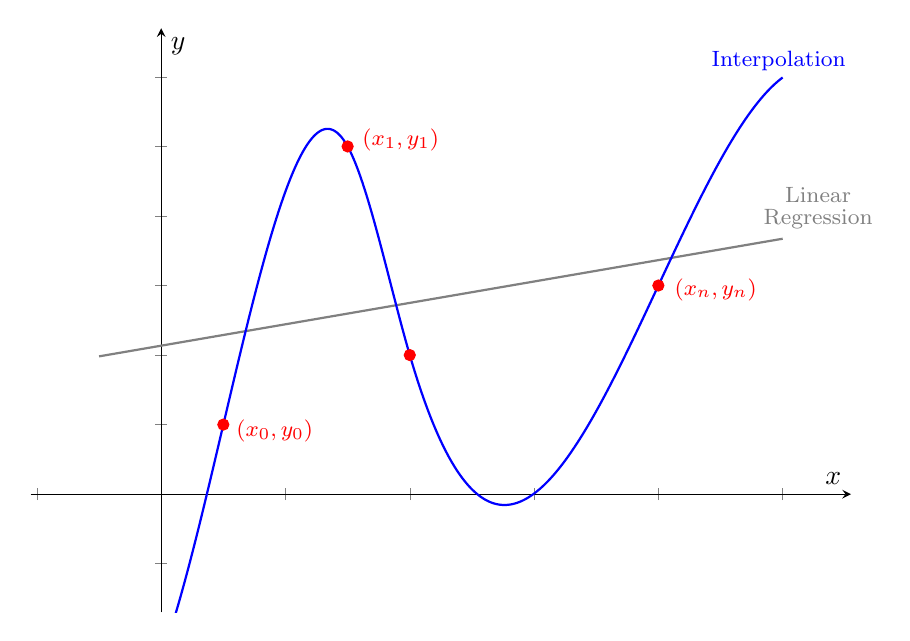
\begin{tikzpicture}
	\node[color=blue] at (9.5,7){\footnotesize{Interpolation}};
	\node[color=gray] at (10,5.3){\footnotesize{Linear}};
	\node[color=gray] at (10,5){\footnotesize{Regression}};
	\node[color=red] at (3.1,2.3) {\footnotesize{$(x_0,y_0)$}};
	\node[color=red] at (4.7,6) {\footnotesize{$(x_1,y_1)$}};
	\node[color=red] at (8.7,4.1) {\footnotesize{$(x_n,y_n)$}};

    \begin{axis}[
        legend pos=south east,
        axis x line=middle,
        axis y line=middle,
	xticklabels=\empty,
	yticklabels=\empty
        grid = none ,
        width=12cm,
        height=9cm,
        grid style={dashed, gray!1},
        xmin=-1,     % start the diagram at this x-coordinate
        xmax= 10,    % end   the diagram at this x-coordinate
        ymin=-1,     % start the diagram at this y-coordinate
        ymax= 6,   % end   the diagram at this y-coordinate
        %axis background/.style={fill=white},
        xlabel=$x$,
        ylabel=$y$,
        %xticklabels={-2,-1.6,...,2},
        %yticklabels={-8,-7,...,8},
        %tick align=outside,
        enlargelimits=true,
        tension=0.08]
        \addplot[domain=-1:10, gray, thick,samples=250] {0.1538*x+2.135}; % Linear Regression
        \addplot[domain=0:3,blue, thick,samples=250] {1+449/118*(x-1)-213/472*(x-1)*(x-1)*(x-1)}; % S0
        \addplot[domain=3:4, blue, thick,samples=125] {5-95/59*(x-3)-639/236*(x-3)*(x-3)+311/236*(x-3)*(x-3)*(x-3)}; % S1
        \addplot[domain=4:10, blue, thick,samples=250] {2-725/236*(x-4)+147/118*(x-4)*(x-4)-49/472*(x-4)*(x-4)*(x-4)}; % S2

       \addplot[red, only marks, mark=*] coordinates {(1,1)(3,5)(4,2)(8,3)};
      %\addlegendentry{$f(x)=x^3$}
    \end{axis}
\end{tikzpicture}
\end{center}

	n+1 data points: $(x_0, y_0), (x_1,y_1), ... (x_n,y_n)$.  We want an interpolating function,
	$y=f(x)$ such that $f(x_i) = y_i$ for all $i = 0, 1, ..., n$ Interpolation Conditions.\\ \\

	A totally different approach is the one using the "least squares" method - fit the function as best as 
	possible to the data. \\

	We start with polynomial interpolation, because polynomials are very simple functions with lots of 
	nice properties:

\begin{itemize}
	\item Can be easily calculated
	\item Continuous and Differentiable everywhere
	\item Versatile
\end{itemize}

\pagebreak

	\noindent \textbf{Example:} Linear interpolation (through two points)

\begin{center}
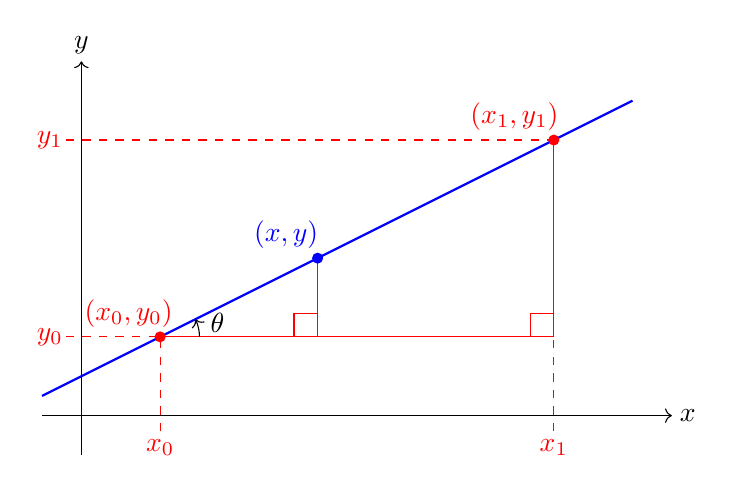
\begin{tikzpicture}
	\coordinate (A) at (6,3.5);
	\coordinate (B) at (3,2);
	\coordinate (C) at (1,1);
	\coordinate (D) at (3,1);
	\coordinate (E) at (6,1);
	\coordinate (O) at (-0.5,0.25);
	\coordinate (o1) at (1,-0.2);
	\coordinate (o3) at (3,-0.2);
	\coordinate (o6) at (6,-0.2);
	\coordinate (o8) at (7,4);
	\coordinate (oC) at (-0.2,1);
	\coordinate (oB) at (-0.2,2);
	\coordinate (oA) at (-0.2, 3.5);
	\coordinate (oX) at (7.5,0);
	\coordinate (oY) at (0,4.5);
	\coordinate (XoY) at (0,0);
	\coordinate (Yo) at (0,-0.5);
	\coordinate (Xo) at (-0.5,0);

	\draw [->](Xo)--(oX);
	\draw [->](Yo)--(oY);
	\draw [blue, thick] (O) -- (o8);
	\draw [red] (C)--(E);
	\draw [red] (D)--(B);
	\draw [red] (E)--(A);
	\draw [red,dashed] (o1)--(C);
	\draw [red,dashed] (o6)--(A);
	\draw [red,dashed] (oC)--(C);
	\draw [red,dashed] (oA)--(A);

 	\fill[red] (intersection of O--A and C--D) circle (2pt);
	\fill[red] (intersection of O--A and E--A) circle (2pt);
	\fill[blue] (intersection of O--A and B--D) circle (2pt);

	\pic [draw, ->, "$\theta$", angle eccentricity=1.5] {angle = E--C--A};
	\tkzMarkRightAngle[draw=red,size=.3](D,E,A);
	\tkzMarkRightAngle[draw=red,size=.3](C,D,B);

	\node[red] (x0y0) at (0.6,1.3) {$(x_0,y_0)$};
	\node[red] (x1y1) at (5.5,3.8) {$(x_1,y_1)$};
	\node[blue] (xnyn) at (2.6,2.3) {$(x,y)$};
	\node (xLabel) at (7.7,0) {$x$};
	\node (yLabel) at (0,4.7) {$y$};
	\node [red](x0) at (1,-0.4) {$x_0$};
	\node [red](x1) at (6,-0.4) {$x_1$};
	\node [red](y0) at (-0.4,1) {$y_0$};
	\node [red](y1) at (-0.4,3.5) {$y_1$};
\end{tikzpicture}
\end{center}




\begin{center}
\begin{tabular}{ccc}
	\underline{Similar Triangles}&&\underline{Two Point Formula for a line}\\ \\
	\Large{$\frac{y-y_0}{x-x_0}$}\, \normalsize{$=$} \,{$\underbrace{\Large{\frac{y_1-y_0}{x_1-x_0}}}_{\text{slope}}$}
		& \Large{$\Leftrightarrow$}
		& $y =$ \Large{$\frac{y_1-y_0}{x_1-x_0}$}\!\! \normalsize{$(x-x_0) + y_0$}\\
	
\end{tabular}
\end{center}

	We distinguish between \textit{Interpolation} and\textit{Extrapolation}.

\begin{center}
\fbox
{
	\parbox{0.8\textwidth}
	{
			\textbf{\underline{Interpolation}:} Calculating points \textit{between} smallest and largest $x_i$ values.\\
			\textbf{\underline{Extrapolation}:} Calculating point \textit{outside} range of $x_i$ values.\\
	
	}
}
\end{center}

\section{Lagrangian Interpolation}


	\noindent \textbf{Example:} Three Data Points $(x_0,y_0)(x_1,y_1)(x_2,y_2)$

\begin{center}
\begin{tikzpicture}
    \begin{axis}[
        legend pos=south east,
        axis x line=middle,
        axis y line=middle,
	every axis x label/.style={at={(current axis.right of origin)},anchor= west},
	every axis y label/.style={at={(current axis.above origin)},anchor= south},
	xticklabels=\empty,
	yticklabels=\empty
        grid = none ,
        width=12cm,
        height=9cm,
        grid style={dashed, gray!1},
        xmin=-0.18,     % start the diagram at this x-coordinate
        xmax= 8,    % end   the diagram at this x-coordinate
        ymin=-0.2,     % start the diagram at this y-coordinate
        ymax= 4,   % end   the diagram at this y-coordinate
        %axis background/.style={fill=white},
        xlabel=$x$,
        ylabel=$y$,
        %xticklabels={-2,-1.6,...,2},
        %yticklabels={-8,-7,...,8},
        %tick align=outside,
        enlargelimits=true,
        tension=0.08]
        \addplot[domain=-0.5:8, blue, thick,samples=250] {0.125*(x-6)*(x-6)+0.5}; % Parabola
 	\addplot[domain=-0.2:2, red, dashed,samples=2] {2.5} node[left, pos=0] {$y_0$}; % y0
	\addplot[domain=-0.2:4, red, dashed,samples=2] {1} node[left, pos=0] {$y_1$}; % y1
	\addplot[domain=-0.2:7, red, dashed,samples=2] {0.625} node[left, pos=0] {$y_2$}; % y2

	\addplot[dashed,red,mark=none] coordinates{(2,-0.2)(2,2.5)} node[below, pos=0] {$x_0$}; %x0
	\addplot[dashed,red,mark=none] coordinates{(4,-0.2)(4,1)} node[below, pos=0] {$x_1$}; %x1
	\addplot[dashed,red,mark=none] coordinates{(7,-0.2)(7,0.625)} node[below, pos=0] {$x_2$}; %x2
 
	\addplot[red, only marks, mark=*] coordinates {(2,2.5)(4,1)(7,0.625)};

    \end{axis}
\end{tikzpicture}
\end{center}

\begin{tabbing}
	Model: \hspace{0.1cm} \= $p(x) = A + Bx + Cx^2$\\
	\> \qquad \quad \,\!\!  $\uparrow$ \quad \,\! $\uparrow$ \quad \;\;\! $\uparrow$\\
	\> \qquad \quad \, parameters
\end{tabbing}

	How do we compute these parameters? Interpolating conditions lead to:

\begin{center}
	$y_0 = p(x_0) = A + Bx_0 + Cx_0 ^{\;2}$\\
	\medskip
	$y_1 = p(x_1) = A + Bx_1 + Cx_1 ^{\;2}$\\
	\medskip
	$y_2 = p(x_2) = A + Bx_2 + Cx_2 ^{\;2}$\\
\end{center}

This is a linear system:

\begin{center}
	$
	\begin{pmatrix}
		1 & x_0 & x_0^{\;2} \\
		1 & x_1 & x_1^{\;2} \\
		1 & x_2 & x_2^{\;2}
	\end{pmatrix}
	$
	\nolinebreak
	$
	\begin{pmatrix}
		A\\
		B\\
		C
	\end{pmatrix}
	$
		=
	$
	\begin{pmatrix}
		y_0\\
		y_1\\
		y_2	
	\end{pmatrix}
	$
\end{center}

\begin{center}
\fbox
{
	\parbox{0.5\textwidth}
	{
	\begin{center}
		A Matrix of the form
		\bigskip
		
			$\begin{pmatrix}
				1 & x_0 & x_0^{\;2} & \cdots & x_0^{\; n}\\
				\vdots & \vdots & \vdots & \ddots & \vdots\\
				1 & x_n & x_n^{\;2} & \cdots & x_n^{\; n}
			\end{pmatrix}$

		\bigskip		
		 is called a \textbf{Vandermonde Matrix}.
	\end{center}
	}
}
\end{center}

\bigskip

	\noindent It's determinant is

\vspace{-0.75cm}

\begin{center}
	\begin{equation*}
		\prod_{i<j}(x_i - x_j)
	\end{equation*}
\end{center}

	\noindent so it will be non-zero when all the $x_i$'s are different. This restriction does not interfere with an interpolation problem,
 	since it also requires different $x_i$'s.

\medskip

\begin{center}
\fbox{
	\parbox{0.8\textwidth}
	{
		\medskip
		\textbf{\underline{Theorem}:} For $n+1$ data points $(x_0, y_0), (x_1, y_1), ... (x_n, y_n)$ there is a unique
		polynomial of degree $n$ interpolating these points.
		\medskip
	}
}
\end{center}

	\noindent This polynomial could be computed by Gaussian Elimination, but usually that leads to numerical problems
	(round-off errors will amplify). \textit{There is a smarter way!}

\begin{center}
\begin{tikzpicture}
    \begin{axis}[
        legend pos=south east,
        axis x line=middle,
        axis y line=middle,
	every axis x label/.style={at={(current axis.right of origin)},anchor=north},
	every axis y label/.style={at={(current axis.above origin)},anchor=east},
	xticklabels=\empty,
	yticklabels=\empty
        grid = none ,
        width=12cm,
        height=9cm,
        grid style={dashed, gray!1},
        xmin=-0.15,     % start the diagram at this x-coordinate
        xmax= 4,    % end   the diagram at this x-coordinate
        ymin=-0.5,     % start the diagram at this y-coordinate
        ymax= 1.5,   % end   the diagram at this y-coordinate
        %axis background/.style={fill=white},
	xlabel=$x$,
        ylabel=$y$,
        %xticklabels={-2,-1.6,...,2},
        %yticklabels={-8,-7,...,8},
        %tick align=outside
        enlargelimits=true,
        tension=0.08]
        \addplot[domain=-0.5:8, blue, thick,samples=250] {(x-2)*(x-3.5)/2.5}; % Parabola
 	\addplot[domain=-0.1:1, red, dashed,samples=2] {1} node[left, pos=0] {1}; % y0


	\draw [thick, gray,decorate,decoration={brace,amplitude=10pt,mirror},xshift=0.4pt,yshift=-0.4pt]
		(axis cs:1,-0.25) -- (axis cs:2,-0.25) node[black,midway,yshift=-0.6cm] {};
	\draw [thick, gray,decorate,decoration={brace,amplitude=10pt,mirror},xshift=0.4pt,yshift=-0.4pt]
		(axis cs:2,-0.25) -- (axis cs:3.5,-0.25) node[black,midway,yshift=-0.6cm] {};


	\addplot[dashed,red,mark=none] coordinates{(1,-0.1)(1,1)} node[below, pos=0] {$x_0$}; %x0
	\addplot[red,mark=none] coordinates{(2,-0.1)} node[below, pos=0] {$x_1$}; %x1
	\addplot[red,mark=none] coordinates{(3.5,-0.1)} node[below, pos=0] {$x_2$}; %x2
	\addplot[mark=none] coordinates{(2.25,-0.4)} node[below, pos=0] {\small Not necessarily equidistant}; %x2
 
	\addplot[red, only marks, mark=*] coordinates {(1,1)(2,0)(3.5,0)};


    \end{axis}
\end{tikzpicture}
	\\
	$L_0(x)=a(x-x_1)(x-x_2)$
\end{center}

	Choose:

\begin{center}
	$a =$ \Large{$\frac{1}{(x_0-x_1)(x_0-x_2)}$}

	\normalsize
	\bigskip

	$\Rightarrow \; L_0(x) =$ \Large{$\frac{(x-x_1)(x-x_2)}{x_0-x_1)(x_0-x_2)}$}

	\normalsize
\end{center}

	So:

\begin{center}
%\begin{math}
$
  \left.
    \begin{array}{l}
	L_0(x_0) = 1\\
	L_0(x_1) = 0\\
	L_0(x_2) = 0
    \end{array}
  \right\}
	\text{This is the \textbf{interpolating parablola}}
$
%\end{math}

	\bigskip


\begin{tikzpicture}
    \begin{axis}[
        legend pos=south east,
        axis x line=middle,
        axis y line=middle,
	every axis x label/.style={at={(current axis.right of origin)},anchor=north},
	every axis y label/.style={at={(current axis.above origin)},anchor=east},
	xticklabels=\empty,
	yticklabels=\empty
        grid = none ,
        width=12cm,
        height=9cm,
        grid style={dashed, gray!1},
        xmin=-0.15,     % start the diagram at this x-coordinate
        xmax= 4,    % end   the diagram at this x-coordinate
        ymin=-0.25,     % start the diagram at this y-coordinate
        ymax= 1.5,   % end   the diagram at this y-coordinate
        %axis background/.style={fill=white},
        xlabel=$x$,
        ylabel=$y$,
        %xticklabels={-2,-1.6,...,2},
        %yticklabels={-8,-7,...,8},
        %tick align=outside
        enlargelimits=true,
        tension=0.08]
        \addplot[domain=-0.5:8, blue, thick,samples=250] {-(x-1)*(x-3.5)/1.5}; % Parabola
 	\addplot[domain=-0.1:2, red, dashed,samples=2] {1} node[left, pos=0] {1}; % y0

	\addplot[dashed,red,mark=none] coordinates{(2,-0.1)(2,1)} node[below, pos=0] {$x_1$}; %x0
	\addplot[red,mark=none] coordinates{(1,-0.1)} node[below, pos=0] {$x_0$}; %x1
	\addplot[red,mark=none] coordinates{(3.5,-0.1)} node[below, pos=0] {$x_2$}; %x2

 
	\addplot[red, only marks, mark=*] coordinates {(1,0)(2,1)(3.5,0)};


    \end{axis}
\end{tikzpicture}

	\bigskip

	$L_1(x)=$ \Large{$\frac{(x-x_0)(x-x_2)}{(x_1-x_0)(x_1-x_2)}$}

	\vspace{1.5cm}
	\normalsize

\begin{tikzpicture}
    \begin{axis}[
        legend pos=south east,
        axis x line=middle,
        axis y line=middle,
	every axis x label/.style={at={(current axis.right of origin)},anchor=north},
	every axis y label/.style={at={(current axis.above origin)},anchor=east},
	xticklabels=\empty,
	yticklabels=\empty
        grid = none ,
        width=12cm,
        height=9cm,
        grid style={dashed, gray!1},
        xmin=-0.15,     % start the diagram at this x-coordinate
        xmax= 4,    % end   the diagram at this x-coordinate
        ymin=-0.25,     % start the diagram at this y-coordinate
        ymax= 1.5,   % end   the diagram at this y-coordinate
        %axis background/.style={fill=white},
        xlabel=$x$,
        ylabel=$y$,
        %xticklabels={-2,-1.6,...,2},
        %yticklabels={-8,-7,...,8},
        %tick align=outside
        enlargelimits=true,
        tension=0.08]
        \addplot[domain=-0.5:8, blue, thick,samples=250] {(x-1)*(x-2)/3.75}; % Parabola
 	\addplot[domain=-0.1:3.5, red, dashed,samples=2] {1} node[left, pos=0] {1}; % y0
%	\addplot[domain=-0.2:4, red, dashed,samples=2] {1} node[left, pos=0] {$y_1$}; % y1
%	\addplot[domain=-0.2:7, red, dashed,samples=2] {0.625} node[left, pos=0] {$y_2$}; % y2


	\addplot[dashed,red,mark=none] coordinates{(3.5,-0.1)(3.5,1)} node[below, pos=0] {$x_2$}; %x0
	\addplot[red,mark=none] coordinates{(1,-0.1)} node[below, pos=0] {$x_0$}; %x1
	\addplot[red,mark=none] coordinates{(2,-0.1)} node[below, pos=0] {$x_1$}; %x2
%	\addplot[mark=none] coordinates{(2.25,-0.4)} node[below, pos=0] {\small Not necessarily equidistant}; %x2
 
	\addplot[red, only marks, mark=*] coordinates {(1,0)(2,0)(3.5,1)};


    \end{axis}
\end{tikzpicture}

	\bigskip
	$L_2(x)=$ \Large{$\frac{(x-x_0)(x-x_1)}{(x_2-x_0)(x_2-x_1)}$}
	\normalsize

\fbox
{
	\parbox{0.75\textwidth}
	{
		Now with $(x_0, \, y_0)$,  $(x_1, \, y_1)$, and  $(x_2, \, y_2)$, the interpolating polynomial is:

		\begin{center}
			$p(x) = y_0 \cdot L_0(x) + y_1 \cdot L_1(x) + y_2 \cdot L_2(x)$
		\end{center}
	}
}

\end{center}

\section{Newtonian Interpolation}
	When data points are "added" the Lagrange polynomials have to be computed all over again. The Newton approach
	is designed in a way that we can use previous calculations when interpolating with additional data points.\\ \\

	\noindent \textbf{Example:} Three Coordinates (1,-2), (2,5), and (-1,-4)\\ \\

	\noindent Align the coordinates in two separate columns:

\begin{center}
	\begin{tabular}{cc}
	$x$ & $y$\\
	\hline
	1 & -2\\
	2 & 5 \\
	-1&-4
	\end{tabular}
\end{center}

	\noindent Subtract the first x-coordinate from each subsequent coordinate, and write the difference in the next column to the left.
	\vspace {-0.4cm}

\begin{center}
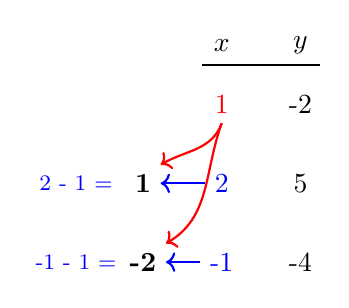
\begin{tikzpicture}
	\node (A) at (1.5,3.25) {$x$};
	\node  (B) [red] at (1.5,2.5){1}; 
	\node (C) [blue] at (1.5,1.5) {2};
	\node (D)[blue] at (1.5,0.5) {-1};
	\node (E) at (0.5,1.5) {\textbf{1}};
	\node (F)  at (0.5,0.5) {\textbf{-2}};
	\node (a) at (2.5,3.25) {$y$};
	\node (b) at (2.5,2.5) {-2};
	\node (c) at (2.5,1.5) {5};
	\node (d) at (2.5,0.5) {-4};

	\draw [->, thick, blue] (C) edge (E) (D) edge (F);
	\draw [->, thick, red] (B.south) to [out=250, in = 30] (E.north east);
	\draw [->, thick, red] (B.south) to  [out=250, in = 30] (F.north east);
	\draw [thick, black] (1.25,3) to (2.75,3);


\footnotesize

	\node [blue] (L1) at (-0.35,0.5) {-1 - 1 =};
	\node [blue]  (L2) at (-0.35,1.5) {2 - 1 =};

\normalsize

\end{tikzpicture}
\end{center}
	
	\noindent In the next column subtract the first value of that column from each subsequent value, just as you did in the
		first column:
	\vspace {-0.4cm}


\begin{center}
\begin{tikzpicture}
	\node (A) at (1.5,3.25) {$x$};
	\node  (B) at (1.5,2.5){1}; 
	\node (C) at (1.5,1.5) {2};
	\node (D) at (1.5,0.5) {-1};
	\node (E) [red] at (0.5,1.5) {1};
	\node (F) [blue] at (0.5,0.5) {-2};
	\node (G) at (-0.5,0.5) {\textbf{-3}};
	\node (a) at (2.5,3.25) {$y$};
	\node (b) at (2.5,2.5) {-2};
	\node (c) at (2.5,1.5) {5};
	\node (d) at (2.5,0.5) {-4};

	\draw [->, thick, blue] (F) edge (G);
	\draw [->, thick, red] (E.south) to [out=250, in = 30] (G.north east);

	\draw [thick, black] (1.25,3) to (2.75,3);


\footnotesize

	\node [blue] (L1) at (-1.35,0.5) {-2 - 1 =};


\normalsize

\end{tikzpicture}
\end{center}

	\noindent Repeat this process until there is a left-most column with only one value.\\

	For the y-coordinates, the process is a bit different. Just like with the x-coordinates, subtract the first value in each column 
	from all subsequent values in that column. Then, divide the resulting difference by the difference of the corresponding
	x-values (i.e. the answers on the left side).

\begin{center}
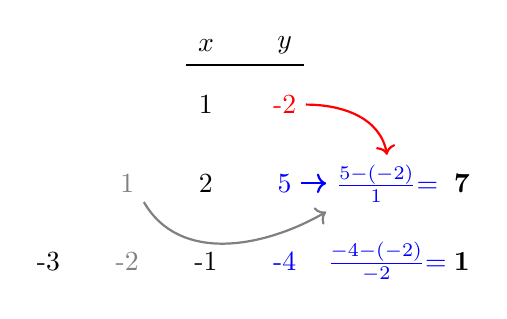
\begin{tikzpicture}
	\node (A) at (1.5,3.25) {$x$};
	\node  (B) at (1.5,2.5){1}; 
	\node (C) at (1.5,1.5) {2};
	\node (D) at (1.5,0.5) {-1};
	\node (E) [gray] at (0.5,1.5) {1};
	\node (F) [gray] at (0.5,0.5) {-2};
	\node (G) at (-0.5,0.5) {-3};
	\node (a) at (2.5,3.25) {$y$};
	\node (b)[red] at (2.5,2.5) {-2};
	\node  (c) [blue] at (2.5,1.5) {5};
	\node  (d) [blue] at (2.5,0.5) {-4};
	\node (e) at (4.75,1.5) {\textbf{7}};
	\node (f) at (4.75,0.5) {\textbf{1}};

	\node(L1)  [blue]  at (3.8,0.5) {$\frac{-4-(-2)}{-2}$=};
	\node (L2) [blue]  at (3.8,1.5) {$\frac{5-(-2)}{1}$=};


	\draw [->, thick, blue] (c) to (L2);
	\draw [->, thick, red] (b.east) to [out=0, in = 100] (L2.north);
	\draw [->, thick, gray] (E.south east) to  [out=300, in = 210] (L2.south west);
	\draw [thick, black] (1.25,3) to (2.75,3);

\normalsize

\end{tikzpicture}
\end{center}

	\noindent Repeat this process until there is a right-most column with only one value:

\begin{center}
\begin{tikzpicture}
	\node (A) at (1.5,3.25) {$x$};
	\node  (B) at (1.5,2.5){1}; 
	\node (C) at (1.5,1.5) {2};
	\node (D) at (1.5,0.5) {-1};
	\node (E)at (0.5,1.5) {1};
	\node (F) at (0.5,0.5) {-2};
	\node (G) [gray] at (-0.5,0.5) {-3};
	\node (a) at (2.5,3.25) {$y$};
	\node (b) at (2.5,2.5) {-2};
	\node  (c) at (2.5,1.5) {5};
	\node  (d) at (2.5,0.5) {-4};
	\node (e) [red] at (3.5,1.5) {7};
	\node (f) [blue] at (3.5,0.5) {1};
	\node (g) at (5.3, 0.5) {\textbf{2}};

	\node(L2)  [blue]  at (4.7,0.5) {$\frac{1-7}{-3}$=};

	\draw [->, thick, blue] (f) to (L2);
	\draw [->, thick, red] (e.east) to [out=0, in = 100] (L2.north);
	\draw [->, thick, gray] (G.south east) to  [out=330, in = 210] (L2.south west);
	\draw [thick, black] (1.25,3) to (2.75,3);

\normalsize

\end{tikzpicture}
\end{center}

	\noindent How do we turn this into a polynomial?

\begin{center}
	\begin{tikzpicture}[square/.style={regular polygon,regular polygon sides=4}]


	\node (A) at (1.5,3.25) {$x$};
	\node  (B) [blue, square, draw] at (1.5,2.5){1}; 
	\node (C) [blue, square, draw] at (1.5,1.5) {2};
	\node (D) at (1.5,0.5) {-1};
	\node (E)at (0.5,1.5) {1};
	\node (F) at (0.5,0.5) {-2};
	\node (G) at (-0.5,0.5) {-3};
	\node (a) at (2.5,3.25) {$y$};
	\node (b) [red, square, draw] at (2.5,2.5) {-2};
	\node  (c) at (2.5,1.5) {5};
	\node  (d) at (2.5,0.5) {-4};
	\node (e) [red, square, draw] at (3.5,1.5) {7};
	\node (f) at (3.5,0.5) {1};
	\node (g) [red, square, draw] at (4.5, 0.5) {2};

	\draw [thick, black] (1.25,3) to (2.75,3);

\normalsize

\end{tikzpicture}
\end{center}

	\noindent Beginning with your first y-coordinate, multiply the first value in each y-column as a coefficient in a polynomial
	of increasing degree, starting with degree 0.  These polynomials will be composed of expressions of $(x-x_{n-1})$  Where
	$x_{n-1}$ are your original x-coordinates. Add these polynomials together for the desired formula:

\begin{tabbing}
	\hspace{3.3cm} \= $p(x)$ \hspace{1mm} \=  $= \red -2 \, \black \cdot \!\!\!\!\!\!\!
	\underbrace{1}_{\text{\footnotesize{degree 0}}} \!\!\!\!\!\!
	+ \; \red 7 \black \underbrace{(x-\blue 1 \black)} _{\text{\footnotesize{degree 1}}}
	+ \; \red 2 \black \underbrace{(x-\blue 1 \black)(x-\blue 2 \black)}_{\text{\footnotesize{degree 2}}}$\\ \\

	\>\>$= -2 + 7x - 7 + 2x^2 - 6x + 4$\\ \\

	\>\>$= 2x^2 + x -5$\\
\end{tabbing}

	What happens if we want to add an additional data-point?\\

	\noindent \textbf{Example:} Three Coordinates (1,-2), (2,5), (-1,-4), and (-2, -11):

\begin{center}
\begin{tikzpicture}[square/.style={regular polygon,regular polygon sides=4}]


	\node (A) at (1.5,3.25) {$x$};
	\node  (B) at (1.5,2.5){\textbf{1}}; 
	\node (C) at (1.5,1.5) {\textbf{2}};
	\node (D) at (1.5,0.5) {\textbf{-1}};
	\node (E) at (1.5, -0.5) {-2};
	\node (F)at (0.5,1.5) {1};
	\node (G) at (0.5,0.5) {-2};

	\node (I) at (-0.5,0.5) {-3};

	\node (a) at (2.5,3.25) {$y$};
	\node (b) at (2.5,2.5) {\textbf{-2}};
	\node  (c) at (2.5,1.5) {\textbf{5}};
	\node  (d) at (2.5,0.5) {\textbf{-4}};
	\node (e)  at (2.5, -0.5) {-11};
	\node (f)  at (3.5,1.5) {7};
	\node (g) at (3.5,0.5) {1};

	\node (i) at (4.5, 0.5) {2};


	\draw [thick, black] (1.25,3) to (2.75,3);

\normalsize

\end{tikzpicture}
\end{center}

	\noindent If we begin building the triangle as we did before, we get the same values we did previously for the first three
	three coordinates. \textit{The same points in the same order will always result in the same triangle.}  Because of this,
	adding a new coordinate just means adding a new row.

\begin{center}
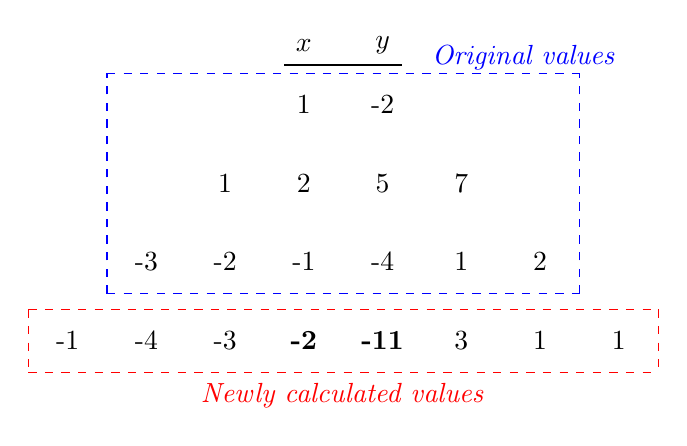
\begin{tikzpicture}[square/.style={regular polygon,regular polygon sides=4}]


	\node (A) at (1.5,3.25) {$x$};
	\node  (B) at (1.5,2.5){1}; 
	\node (C) at (1.5,1.5) {2};
	\node (D) at (1.5,0.5) {-1};
	\node (E) at (1.5, -0.5) {\textbf{-2}};
	\node (F)at (0.5,1.5) {1};
	\node (G) at (0.5,0.5) {-2};
	\node (H) at (0.5, -0.5) {-3};
	\node (I) at (-0.5,0.5) {-3};
	\node (J) at (-0.5, -0.5) {-4};
	\node (K) at (-1.5, -0.5) {-1};
	\node (a) at (2.5,3.25) {$y$};
	\node (b) at (2.5,2.5) {-2};
	\node  (c) at (2.5,1.5) {5};
	\node  (d) at (2.5,0.5) {-4};
	\node (e)  at (2.5, -0.5) {\textbf{-11}};
	\node (f)  at (3.5,1.5) {7};
	\node (g) at (3.5,0.5) {1};
	\node (h) at (3.5,-0.5) {3};
	\node (i) at (4.5, 0.5) {2};
	\node (j) at (4.5, -0.5) {1};
	\node (k) at (5.5, -0.5) {1};
	\node (l)[red] at (2, -1.2) {\textit{Newly calculated values}};
	\node (m) [blue] at (4.3, 3.1) {\textit{Original values}};

	\draw [thick, black] (1.25,3) to (2.75,3);
	\draw [red, dashed] (-2,-0.1) to (6,-0.1);
	\draw [red, dashed] (-2,-0.9) to (6,-0.9);
	\draw [red, dashed] (-2,-0.1) to (-2,-0.9);
	\draw [red, dashed] (6,-0.1) to (6,-0.9);
	\draw [blue, dashed] (-1, 0.1) to (5, 0.1);
	\draw [blue, dashed] (-1, 2.9) to (5, 2.9);
	\draw [blue, dashed] (-1, 0.1) to (-1, 2.9);
	\draw [blue, dashed] (5, 0.1) to (5, 2.9);
\normalsize

\end{tikzpicture}
\end{center}


	\noindent Repeat the process from the first three coordinates for the new coordinate to obtain fourth row to the triangle.
	Just as we were able to add the new coordinates to the last row of the triangle, we can append the new calculated values
	to the end of our previously obtained polynomial:

\begin{center}
\begin{tikzpicture}[square/.style={regular polygon,regular polygon sides=4}]


	\node (A) at (1.5,3.25) {$x$};
	\node  (B) [square, draw] at (1.5,2.5){1}; 
	\node (C) [square, draw] at (1.5,1.5) {2};
	\node (D) [blue, square, draw] at (1.5,0.5) {-1};
	\node (E) at (1.5, -0.5) {-2};
	\node (F)at (0.5,1.5) {1};
	\node (G) at (0.5,0.5) {-2};
	\node (H) at (0.5, -0.5) {-3};
	\node (I) at (-0.5,0.5) {-3};
	\node (J) at (-0.5, -0.5) {-4};
	\node (K) at (-1.5, -0.5) {-1};
	\node (a) at (2.5,3.25) {$y$};
	\node (b) [square, draw] at (2.5,2.5) {-2};
	\node  (c) at (2.5,1.5) {5};
	\node  (d) at (2.5,0.5) {-4};
	\node (e)  at (2.5, -0.5) {-11};
	\node (f)  [square, draw] at (3.5,1.5) {7};
	\node (g) at (3.5,0.5) {1};
	\node (h) at (3.5,-0.5) {3};
	\node (i) [square, draw] at (4.5, 0.5) {2};
	\node (j) at (4.5, -0.5) {1};
	\node (k) [red, square, draw] at (5.5, -0.5) {1};

	\draw [thick, black] (1.25,3) to (2.75,3);
\normalsize

\end{tikzpicture}
	\vspace{0.5cm}\\
	$p(x) = \underbrace{-2 \cdot 1 + 7(x-1) + 2(x-1)(x-2)}_{\text{\footnotesize{previously obtained}}} + \; \red 1 \black \cdot
	(x-1)(x-2)(x-(\blue -1 \black))$
\end{center}

	\noindent So we see that while the Newton method of interpolation is a bit complicated, it has the nice property of
	allowing us to add more points of data without having to recalculate our previous values.

\section {Interpolating Non-Polynomial Functions}

\noindent \textbf{Example:} Use data points from the function $f(x) =$ \large{$\frac{1}{1+25x^2}$}:

\begin{center}
	\begin{tabular}{c|c|c|c|c|c|c}
		$x$ & $\pm 1$ & $\pm 0.8$ & $\pm 0.6$ & $\pm 0.4$ & $\pm0.2$ & 0\\
		\hline
		$f(x)$ & 0.038 & 0.058 & $\frac{1}{10}$ & $\frac{1}{5}$ &  $\frac{1}{2} $ & 1
	\end{tabular}
\end{center}

\begin{figure}[!htb]
	% r - right
	% l - left
	% o - outside edge
	% i - inside edge
	\center{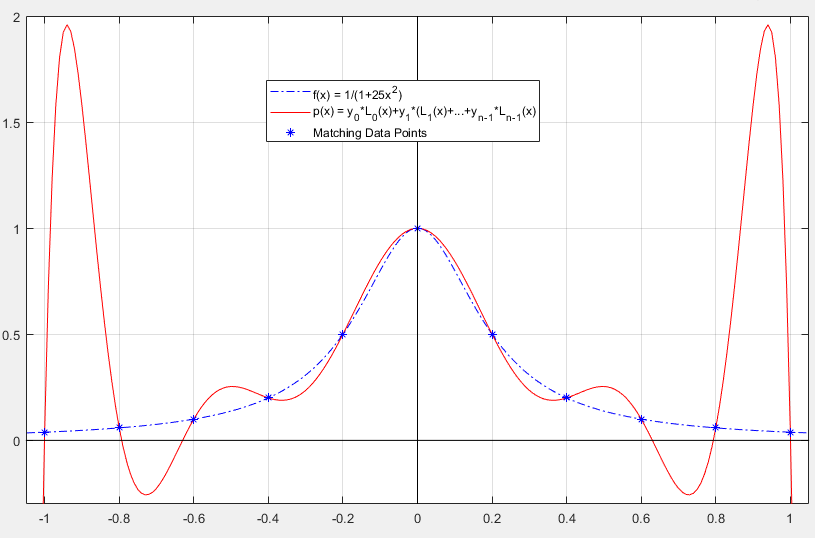
\includegraphics[width=0.8\linewidth]{Oscillations1.png}}

	\caption{We observe high oscillations between the interpolated data points.}\label{fig:Oscillations 1}
\end{figure}
\FloatBarrier

	\noindent \normalsize What is going on here?
	\begin{itemize}
		\item We try to reconstruct a function that has non-polynomial behavior (horizontal asymptote).
		\item Equidistant points create extra trouble.  \textit{Cluster points at the end points to obtain better results.}
	\end{itemize}

	 \noindent Let's try more midpoints: $0, \,\pm0.1, \,\pm0.2...\,\pm1$. Now we have 21 points instead of 11:

\begin{figure}[!htb]
	% r - right
	% l - left
	% o - outside edge
	% i - inside edge
	\center{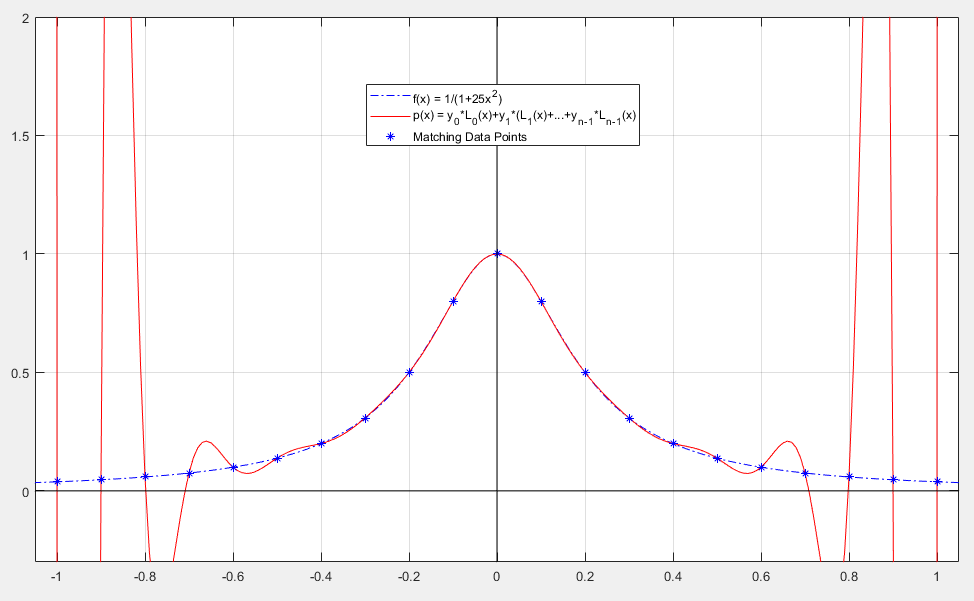
\includegraphics[width=0.8\linewidth]{Oscillations2.png}}

	\caption{Increasing the number of points leads to more oscillations.}\label{fig:Oscillations 2}
\end{figure}
\FloatBarrier

\section{Spline Interpolation}

	\noindent Increasing the number of data points in our interpolating polynomial leads to worse results.  What is a practical solution?
	We could try using piecewise interpolation with small degree polynomials.  The simplest case of this would be piecewise linear
	 interpolation.

\begin{center}
\begin{tikzpicture}
    \begin{axis}[
        legend pos=south east,
        axis x line=middle,
        axis y line=middle,
	xticklabels=\empty,
	yticklabels= \empty,
	xtick={-1,-0.8,-0.6,-0.4,-0.2,0.2,0.4,0.6,0.8, 1},
	ytick={0.25,0.5,0.75,1},
        grid = none ,
        width=15cm,
        height=9cm,
        grid style={dashed, gray!1},
        xmin=-1.2,     % start the diagram at this x-coordinate
        xmax= 1.2,    % end   the diagram at this x-coordinate
        ymin=-0.05,     % start the diagram at this y-coordinate
        ymax= 1,   % end   the diagram at this y-coordinate
        %axis background/.style={fill=white},
        xlabel=$x$,
        ylabel=$y$,
        enlargelimits=true,
        tension=0.08]
 
	\addplot[domain=-1.3:1.3, gray,thick, samples=125] {1/(1+25*x*x};


   \addplot[blue, thick,] coordinates {(-1,0.0385)(-0.8,0.0588)(-0.6,0.1)(-0.4,0.2)(-0.2,0.5)(0,1)(0.2,0.5)(0.4,0.2)(0.6,0.1)(0.8,0.0588)(1,0.0385)};

   \addplot[blue, only marks, mark=*] coordinates {(-1,0.0385)(-0.8,0.0588)(-0.6,0.1)(-0.4,0.2)(-0.2,0.5)(0,1)(0.2,0.5)(0.4,0.2)(0.6,0.1)(0.8,0.0588)(1,0.0385)};
 

	\node(x1) at (axis cs: 1, -0.075){1};
	\node(x2) at (axis cs: -1, -0.075){-1};
	\node(y1) at (axis cs: -0.1, 1){1};
    \end{axis}
\end{tikzpicture}
\end{center}

	\noindent \textbf{Piecewise Linear} interpolation gets rid of oscillations and is continuous, but usually isn't differentiable
	at the interpolating points.

\begin{center}
	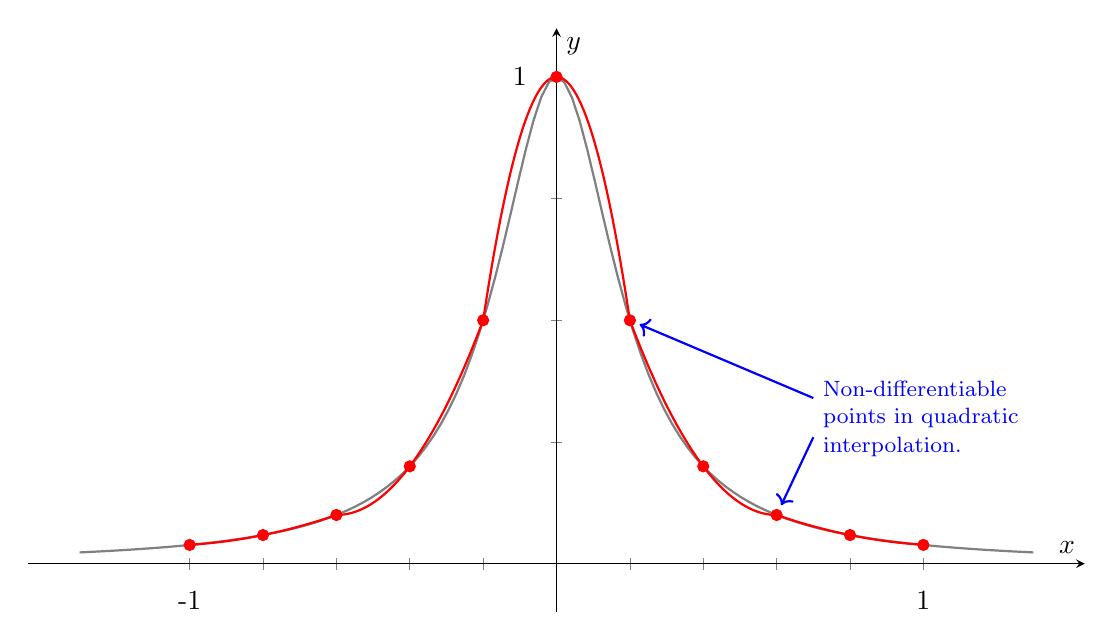
\begin{tikzpicture}

    \begin{axis}[
        legend pos=south east,
        axis x line=middle,
        axis y line=middle,
	xticklabels=\empty,
	yticklabels= \empty,
	xtick={-1,-0.8,-0.6,-0.4,-0.2,0.2,0.4,0.6,0.8, 1},
	ytick={0.25,0.5,0.75,1},
        grid = none ,
        width=15cm,
        height=9cm,
        grid style={dashed, gray!1},
        xmin=-1.2,     % start the diagram at this x-coordinate
        xmax= 1.2,    % end   the diagram at this x-coordinate
        ymin=0,     % start the diagram at this y-coordinate
        ymax= 1,   % end   the diagram at this y-coordinate
        %axis background/.style={fill=white},
        xlabel=$x$,
        ylabel=$y$,
        enlargelimits=true,
        tension=0.08]
	\addplot[domain=-1.3:1.3, gray,thick, samples=125] {1/(1+25*x*x};

	\addplot[domain=-0.2:0.2, red, thick, samples=125] {-12.5*x*x+1};

	\addplot[domain=0.2:0.6, red, thick, samples=125] {6.25*(x-0.4)*(x-0.6)-5*(x-0.2)*(x-0.6)+1.25*(x-0.2)*(x-0.4)};
	\addplot[domain=-0.6:-0.2, red, thick, samples=125] {6.25*(x+0.4)*(x+0.6)-5*(x+0.2)*(x+0.6)+1.25*(x+0.2)*(x+0.4)};

	\addplot[domain=0.6:1, red, thick, samples=125] {1.25*(x-0.8)*(x-1)-1.47*(x-0.6)*(x-1)+0.485*(x-0.6)*(x-0.8)};
	\addplot[domain=-1:-0.6, red, thick, samples=125] {1.25*(x+0.8)*(x+1)-1.47*(x+0.6)*(x+1)+0.485*(x+0.6)*(x+0.8)};


   \addplot[red, only marks, mark=*] 
	coordinates {(-1,0.0385)(-0.8,0.0588)(-0.6,0.1)(-0.4,0.2)(-0.2,0.5)(0,1)(0.2,0.5)(0.4,0.2)(0.6,0.1)(0.8,0.0588)(1,0.0385)};


	\node(x1) at (axis cs: 1, -0.075){1};
	\node(x2) at (axis cs: -1, -0.075){-1};
	\node(y1) at (axis cs: -0.1, 1){1};
	\node(nd1) at (axis cs: 0.2, 0.5){};
	\node(nd2) at (axis cs: 0.6, 0.1){};
	\node(nd3) [right, blue] at (axis cs: 0.7, 0.36){\footnotesize{Non-differentiable}};
	\node(nd4) [right, blue] at (axis cs: 0.7, 0.3){\footnotesize{points in quadratic}};
	\node(nd5) [right, blue] at (axis cs: 0.7, 0.24){\footnotesize{interpolation.}};

	\draw [->, thick, blue] (nd4.south west) -- (nd2);
	\draw [->,thick, blue] (nd4.north west) -- (nd1);

    \end{axis}
\end{tikzpicture}
\end{center}
	\noindent \textbf{Piecewise Quadratic} interpolation has better curvature, much closer to the original function.  Unlike 
	piecewise linear interpolation it's differentiable at every other point.  Piecewise quadratic interpolation is popular for
	approximate integration Use function values and integrate the interpolating parabola's. (\textit{Simpson's Rule}).

\begin{center}
\begin{tikzpicture}
    \begin{axis}[
        legend pos=south east,
        axis x line=middle,
        axis y line=middle,
      axis line style={draw=none},
      tick style={draw=none},
	xticklabels=\empty,
	yticklabels=\empty
        grid = none ,
        width=12cm,
        height=6cm,
        grid style={dashed, gray!1},
        xmin=-6,     % start the diagram at this x-coordinate
        xmax= 6,    % end   the diagram at this x-coordinate
        ymin=-0.75,     % start the diagram at this y-coordinate
        ymax= 1.5,   % end   the diagram at this y-coordinate
        %axis background/.style={fill=white},
        xlabel=\empty,
        ylabel=\empty,
        %xticklabels={-2,-1.6,...,2},
        %yticklabels={-8,-7,...,8},
        %tick align=outside,
        enlargelimits=true,
        tension=0.08]
      \addplot[domain=-7:-3, blue, thick,samples=250] {1-3/8*(x+6)+1/216*(x+6)^3};

	\addplot[domain=-3:3, blue, thick,samples=250] {-1/4*(x+3)+1/24*(x+3)^2};
	\addplot[domain=3:7, blue, thick,samples=250] {1/4*(x-3)+1/24*(x-3)^2-1/216*(x-3)^3};
  
	\addplot[red, only marks, mark=*] coordinates {(-6.1,0.95)(-5.9,1.05)(-3.05,-0.0625)(-2.9,0.05)(3.05,-0.0625)(2.9,0.05)(6.1,0.95)(5.9,1.05)};
    \end{axis}
\end{tikzpicture}
\end{center}

	\noindent The term \textit{spline} comes from historic ship building methods, which involved bending long flexible wooden
	beams into place, using pins.  \textbf{Spline Interpolation} is a type of piecewise polynomial interpolation, in which the function
	values, derivatives, curvature, etc. at each of the interpolating points.

	The standard method is \textbf{Cubic Spline Interpolation}, which uses 3rd order polynomials with matching function values,
	slope, and curvature.

\bigskip

\noindent \textbf{Example:} 3 points: (-1, 1) (0, 2) (1, 0)

\begin{center}
\begin{tikzpicture}
    \begin{axis}[
        legend pos=south east,
        axis x line=middle,
        axis y line=middle,
  %    axis line style={draw=none},
  %    tick style={draw=none},
	xticklabels=\empty,
	yticklabels=\empty
        grid = none ,
        width=8cm,
        height=8cm,
        grid style={dashed, gray!1},
        xmin=-1.75,     % start the diagram at this x-coordinate
        xmax= 1.75,    % end   the diagram at this x-coordinate
        ymin=-1.25,     % start the diagram at this y-coordinate
        ymax= 2.25,   % end   the diagram at this y-coordinate
        %axis background/.style={fill=white},
        xlabel=$x$,
        ylabel=$y$,
        %xticklabels={-2,-1.6,...,2},
        %yticklabels={-8,-7,...,8},
        %tick align=outside,
        enlargelimits=true,
        tension=0.08]

 
	\addplot[red, only marks, mark=*] coordinates {(-1,1)(0,2)(1,-1)};
	\draw [thick, gray,decorate,decoration={brace,amplitude=10pt,mirror},xshift=0.4pt,yshift=-0.4pt]
		(axis cs:-1,0) -- (axis cs:0,0) node[black,midway,yshift=-0.6cm] {};
	\draw [thick, gray,decorate,decoration={brace,amplitude=10pt,mirror},xshift=0.4pt,yshift=-0.4pt]
		(axis cs:0,0) -- (axis cs:1,0) node[black,midway,yshift=-0.6cm] {};

	\node(x0) at (axis cs: -0.3, 2){2};
	\node(s0) [gray] at (axis cs: -0.5, -0.6){\footnotesize{$s_0(x)$}};
	\node(s1) [gray] at (axis cs: 0.5, -0.6){\footnotesize{$s_1(x)$}};
	\node(x2) at (axis cs: 1, -0.3){1};
    \end{axis}
\end{tikzpicture}
\end{center}

	\noindent  The interpolated function will be composed of the following splines:

\begin{center}
	$s_0(x)=ax^3+bx^2+cx+d$ on [-1,0]\\
	$s_1(x)=ex^3+fx^2+gx+h$ on [0,1]
\end{center}

	\noindent We must determine eight parameters:


\begin{center} 
 $s_0(x_0)=y_0 \quad \Rightarrow \; s_0(-1)=1 \;\;\,$\\
\end{center}
 \vspace{-3mm}
$
  \left.
    \begin{array}{c}
\qquad \qquad \qquad \qquad \;\; s_0(x_1)=y_1 \quad \Rightarrow \quad s_0(0)=2\\
\qquad \qquad \qquad	\qquad \;\; s_1(x_1)=y_1 \quad \Rightarrow \quad s_1(0)=2
    \end{array}
  \right\}
	\text{Matching Values}
$\\
\begin{center}
\vspace{-5mm}
$s_1(x_2)=y_2 \quad \Rightarrow \; s_1(1)=-1\;\;\,$\\
\end{center}
\medskip
	\noindent Matching slope at $x_1$:\\
\begin{center}
\vspace{-7mm}
	$s_0\,'(x_1)=s_1\,'(x_1) \quad \Rightarrow \quad s_0\,'(0) = s_1\,'(0)$
\end{center}

\medskip
	\noindent Matching "Curvature":\\
\begin{center}
\vspace{-7mm}
	$s_0\,''(x_1)=s_1\,''(x_1) \quad \Rightarrow \quad s_0\,''(0) = s_1\,''(0)$
\end{center}
\medskip

	\noindent Two conditions remain.  There are several approaches to "fix" these conditions:
\begin{center}
	$s_0\,''(x_0)=0\qquad s_1\,''(0) = s_1\,''(x_2)=0$
\end{center}

	\noindent This is referred to as \textbf{Natural Cubic Splines}.  The curvature at the endpoints is zero.
	This mimics the behavior of the wooden beams in ship building.\\


%ASK PROFESSOR KEHREIN - First or second derivative!----------------------------------------------------------------------------------------------------------
%----------------------------------------------------------------------------------------------------------------------------------------------------------------------------------
	With \textbf{Clamped Splines} the second derivative of each of the endpoint set to a specified value.
\begin{center}
\vspace{-2mm}
	$s_0\,''(x_0)=\text{[some value]} \qquad s_1\,''(0) = s_1\,''(x_2)=\text{[some value]}$
\end{center}

	\textbf{Periodic Conditions} can also be specified to match the end points of the interpolated function into one that
	is periodic.\\

	In our example, let's find the natural cubic spline:
\begin{center}
	$s_0\,'(x)=3ax^2+2bx+c$\\
	$s_0\,''(x)=6ax+2b$\\
	$s_1\,'(x)=3ex^2+2fx+g$\\
	$s_1\,''(x)=6ex+2fx$\\
\end{center}

\underline{Interpolation Conditions}:
\begin{center}
	$s_0(-1) = a\cdot(-1)^3+b\cdot(-1)^2+c\cdot(-1)+d = 1$\\
	\medskip
	$\Rightarrow \textbf{-a\,+b\,-\,c\,+\,d = 1}$\\
	\bigskip
	$s_0(0) = a \cdot 0^3 + b \cdot 0^2 + c \cdot 0 + d = 2$\\
	\medskip
	$\Rightarrow \textbf{d = 2}$\\
	\bigskip
	$s_1(0) = e \cdot 0^3 + f \cdot 0^2 + g \cdot 0 + h = 2$\\
	\medskip
	$\Rightarrow \textbf{h = 2}$\\
	\bigskip
	$s_1 = e\cdot1^3+f\cdot1^2+g\cdot1+h = -1$\\
	\medskip
	$\Rightarrow \textbf{e\,+\,f\,+\,g\,+\,h = -1}$
\end{center}

\underline{Matching Slope}:
\begin{center}
	$s_0\,'(0) = s_1\,'(0)$\\
	\medskip
	$\Rightarrow 3a \cdot 0^2 + 2b \cdot 0 + c = 3e \cdot 0^2 + 2f \cdot 0 + g$\\
	\medskip
	$\Rightarrow \textbf{c = g}$
\end{center}

\underline{Matching Curvature}:
\begin{center}
	$s_0\,''(0) = s_1\,''(0)$\\
	\medskip
	$\Rightarrow 6a \cdot 0 + 2b = 6e \cdot 0 + 2f$
	\medskip
	$\Rightarrow 2b = 2f$
	\medskip
	$\Rightarrow \textbf{b = f}$
\end{center}

\underline{Natural Conditions}:
\begin{center}
	$s_0\,''(-1) = 6a \cdot (-1) + 2b = 0$\\
	\medskip
	$\Rightarrow \textbf{-6a\,+\,2b=0}$\\
	\bigskip
	$s_0\,''(1) = 6e \cdot 1 + 2f = 0$\\
	\medskip
	$\Rightarrow \textbf{6e\,+\,2f=0}$
\end{center}

	\noindent This leads to a linear system with eight equations for eight unknowns.  In this spline set up, this system has a unique solution.

\begin{center}


\fbox
{
	\parbox{0.4\textwidth}
	{
		\begin{center}
			$-a\,+b\,-\,c\,+\,d = 1$\\
			$d = 2$\\
			$h = 2$\\
			$e\,+\,f\,+\,g\,+\,h = -1$\\
			$c = g$\\
			$b = f$\\
			$-6a\,+\,2b=0$\\
			$6e\,+\,2f=0$
		\end{center}
	}
}

\end{center}

%	\noindent Because some of the coefficients have already been shown to be equal, and $d$ and $h$ have already been solved we can reduce this
%	system of equations down to:
%\begin{center}
%\fbox
%{
%	\parbox{0.4\textwidth}
%	{
%		\begin{center}
%		$-a+b-c = -1$\\
%		$b + c + e = -3$\\
%		$-6a +2b = 0 $\\
%		$2b + 6e = 0$
%		\end{center}
%	}
%}
%\end{center}

	\noindent Through Gaussian Elimination we find the solutions:
\begin{center}
\fbox
{
	\parbox{0.4\textwidth}
	{
	\begin{center}
		$a = -\frac{4}{5}$\\
		\medskip
		$b = f = - \frac{72}{25}$\\
		\medskip
		$c = g = -\frac{-27}{25}$\\
		\medskip
		$d = h = 2$\\
		\medskip
		$e = \frac{24}{25}$\\
	\end{center}
	}
}
\end{center}

	\noindent When we plug these values into our original equations, we get the following:
\begin{center}
	$s_0(x) = -\frac{4}{5}x^3 - \frac{72}{25}x^2 - \frac{27}{25}x + 2$\\
	\bigskip
	$s_1(x) = \frac{24}{25}x^3 - \frac{72}{25}x^2 - \frac{27}{25}x + 2$\\
	\bigskip
\begin{tikzpicture}
    \begin{axis}[
        legend pos=south east,
        axis x line=middle,
        axis y line=middle,
	xticklabels=\empty,
	yticklabels=\empty
        grid = none ,
        width=12cm,
        height=12cm,
        grid style={dashed, gray!1},
        xmin=-1.75,     % start the diagram at this x-coordinate
        xmax= 1.75,    % end   the diagram at this x-coordinate
        ymin=-1.25,     % start the diagram at this y-coordinate
        ymax= 2.25,   % end   the diagram at this y-coordinate
        xlabel=$x$,
        ylabel=$y$,
        enlargelimits=true,
        tension=0.08]
     \addplot[domain=-1:0, blue, thick,samples=250] {-4/5*x^3-72/25*x^2-27/25*x+2};
  \addplot[domain=0:1, green, thick,samples=250] {24/25*x^3-72/25*x^2-27/25*x+2};

 
	\addplot[red, only marks, mark=*] coordinates {(-1,1)(0,2)(1,-1)};


	\node(x0) at (axis cs: -0.3, 2){2};
	\node(s0) [blue] at (axis cs: -1.3, 1.5){$s_0(x)$};
	\node(s1) [green] at (axis cs: 1.1, 0.75){$s_1(x)$};
	\node(x2) at (axis cs: 1, -0.3){1};


    \end{axis}
\end{tikzpicture}


\end{center}

% REVIEW THIS SECTION FOR PHRASING (notes are a bit sparse)
% Should we have proof for Spline Formula?-------------------------------------------------------------------------------------------------------------------------------

%	\begin{center}
%	\fbox
%	{
%		\parbox{0.8\textwidth}
%		{
%		\noindent Formula for $s_k(x)$, using $(x_k, y_k)$:
%		\begin{center}
%			$s_k = y_k + \Big[ \frac{y_{k+1}-y_k}{x_{k+1}-x_k} - (x_{k+1} - x_k) \frac{2z_k + z_{k+1}}{6}\Big](x-x_k)$\\
%			\medskip
%			$+ z_k \frac{(x-x_k)^2}{2} + \frac{z_{k+1}-z_k}{x_{k+1}-x_k}\cdot \frac{(x-x_k)^3}{6}$\\
%		\end{center}
%			For $k=0, ... ,\, n-1$\\ \\

%			With:
%		\begin{center}
%		$z_k = s_{k-1}\, ''(x_k) \qquad k = 1,...,n$\\
%		\medskip
%		$\quad \; z_k = s_k\, ''(x_k) \qquad \quad k = 0, ... n-1$
%		\end{center}
%		}
%	}
%	\end{center}

\pagebreak
	In the preceding example, we had 3 data points, with 2 interpolating spline sections in between them.  This process can be generalized to include 
	more data points and more sections:

	\begin{center}
	\fbox
	{
		\parbox{0.8\textwidth}
		{
		\noindent \textbf{\underline{Requirements for calculating Cubic Splines}}
			\begin{center}
				$(n+1)$ data points $\quad \Rightarrow \quad s_k(x)$ on $[x_k, x_{k+1}]$\\
				\medskip
				for $k = 0. 1, ..., n\!-\!1$
			\end{center}
			\noindent $4\cdot n$ coefficients:
			\begin{itemize}
				\item $2n$ \textit{Interpolation Conditions}
				\item $n-1$ \textit{Slope Conditions} for each "internal point"
				\item $n-1$ \textit{Curvature Conditions} for each internal point
			\end{itemize}
			$\Rightarrow \quad 4n - 2$ conditions.\\

			The two remaining "end" conditions can be determined to fit the nature of the data (i.e. "natural" splines, clamped, periodic, etc.)
		}
	}
	\end{center}
	\bigskip

	To find formulas we start with the second derivative of the spline, which is a continuous, piecewise linear function.

\begin{center}
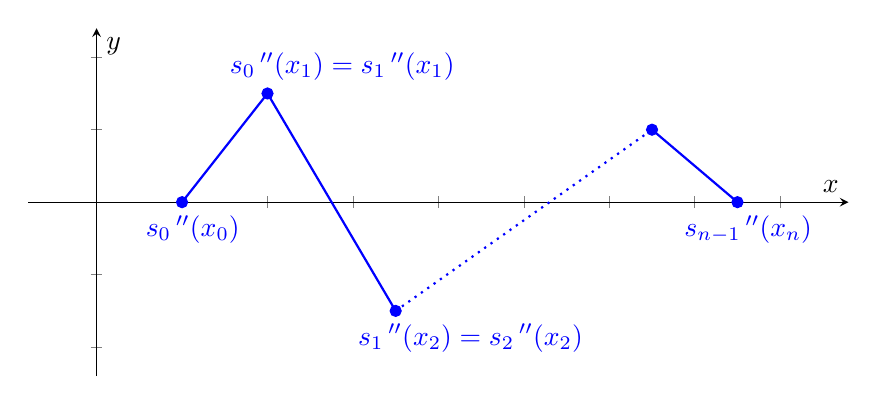
\begin{tikzpicture}
    \begin{axis}[
        legend pos=south east,
        axis x line=middle,
        axis y line=middle,
	xticklabels=\empty,
	yticklabels= \empty,
        grid = none ,
        width=12cm,
        height=6cm,
        grid style={dashed, gray!1},
        xmin=0,     % start the diagram at this x-coordinate
        xmax= 16,    % end   the diagram at this x-coordinate
        ymin=-4,     % start the diagram at this y-coordinate
        ymax= 4,   % end   the diagram at this y-coordinate
        %axis background/.style={fill=white},
        xlabel=$x$,
        ylabel=$y$,
        enlargelimits=true,
        tension=0.08]


  \addplot[blue, only marks, mark=*] coordinates {(2,0)(4,3)(7,-3)(13,2)(15,0)};
  \draw [blue,thick] (axis cs: 2,0) -- (axis cs: 4,3);
  \draw [blue,thick] (axis cs: 4,3) -- (axis cs: 7,-3);
  \draw [blue,thick,dotted] (axis cs: 7,-3) -- (axis cs: 13,2);
  \draw [blue,thick] (axis cs: 13,2) -- (axis cs: 15,0);
      

	\node(x0)[blue] at (axis cs: 2.25, -0.75){$s_0\,''(x_0)$};
	\node(x1)[blue] at (axis cs: 5.75,3.75){$s_0\,''(x_1)= s_1\,''(x_1)$};
	\node(x2)[blue] at (axis cs: 8.75,-3.75){$s_1\,''(x_2)= s_2\,''(x_2)$};
	\node(xn)[blue] at (axis cs: 15.25, -0.75){$s_{n-1}\,''(x_n)$};
    \end{axis}
\end{tikzpicture}
\end{center}

	\noindent Rename the unknown second derivatives at $x_k$ to $z_k$:

\begin{center}
\begin{tikzpicture}
    \begin{axis}[
        legend pos=south east,
        axis x line=middle,
        axis y line=middle,
	xticklabels=\empty,
	yticklabels= \empty,
        grid = none ,
        width=12cm,
        height=6cm,
        grid style={dashed, gray!1},
        xmin=0,     % start the diagram at this x-coordinate
        xmax= 16,    % end   the diagram at this x-coordinate
        ymin=-4,     % start the diagram at this y-coordinate
        ymax= 4,   % end   the diagram at this y-coordinate
        xlabel=$x$,
        ylabel=$y$,
        enlargelimits=true,
        tension=0.08]


  \addplot[red, only marks, mark=*] coordinates {(2,0)(4,3)(7,-3)(13,2)(15,0)};
  \draw [blue,thick] (axis cs: 2,0) -- (axis cs: 4,3);
  \draw [blue,thick] (axis cs: 4,3) -- (axis cs: 7,-3);
  \draw [blue,thick,dotted] (axis cs: 7,-3) -- (axis cs: 13,2);
  \draw [blue,thick] (axis cs: 13,2) -- (axis cs: 15,0);
      

	\node(x0)[red] at (axis cs: 2, -0.75){$z_0$};
	\node(x1)[red] at (axis cs: 4,3.75){$z_1$};
	\node(x2)[red] at (axis cs: 7,-3.75){$z_2$};
	\node(x3)[red] at (axis cs: 15, -0.75){$z_{n-1}$};
    \end{axis}
\end{tikzpicture}

\bigskip




\begin{tikzpicture}

    \begin{axis}[
        legend pos=south east,
        axis x line=middle,
        axis y line=middle,
	xticklabels=\empty,
	yticklabels= \empty,
        grid = none ,
        width=6cm,
        height=6cm,
        grid style={dashed, gray!1},
        xmin=-1,     % start the diagram at this x-coordinate
        xmax= 7,    % end   the diagram at this x-coordinate
        ymin=-1,     % start the diagram at this y-coordinate
        ymax= 7,   % end   the diagram at this y-coordinate
        xlabel=$x$,
        ylabel=$y$,
        enlargelimits=true,
        tension=0.08]


  \addplot[red, only marks, mark=*] coordinates {(3,3)(6,5)};
  \draw [red,dashed] (axis cs: -0.1,3) -- (axis cs: 3,3);
  \draw [red,dashed] (axis cs: -0.1,5) -- (axis cs: 6,5);
  \draw [red,dashed] (axis cs: 3,-0.15) -- (axis cs: 3,3);
  \draw [red,dashed] (axis cs: 6,-0.15) -- (axis cs: 6,5);
      

	\node(zk)[red] at (axis cs: -0.6, 3){$z_k$};
	\node(zk1)[red] at (axis cs: -0.9, 5){$z_{k+1}$};
	\node(xk)[red] at (axis cs: 3,-0.5){$x_k$};
	\node(xk1)[red] at (axis cs: 6,-0.5){$x_{k+1}$};
    \end{axis}
\end{tikzpicture}
\linebreak
	
 	$s_k\, ''(x)= z_k \, +$ \large $\frac{z_{k+1}-z_k}{x_{k+1}-x_k}$

\end{center}
\medskip

	\noindent We can abbreviate the expression $x_{k+1}-x_k$ as $\Delta_k$, resulting in:

\begin{center}
	
	$s_k\, ''(x)= z_k \, +$ \large$\frac{z_{k+1}-z_k}{\Delta_k}$
\end{center}

	\noindent Integrate:
% SUBPROBLEM???--------------------------------------------------------------------------------------------------------------------------------------------------------------
\begin{center}
	
	$s_k\, '(x) = C_k + z_k(x-x_k) + $ \large $\frac{z_{k+1}-z_k}{\Delta_k} \cdot \frac{(x-x_k)^2}{6} $
\end{center}

	\noindent Integrate once more:

\begin{center}
	$s_k(x) = D_k +  C_k(x-x_k) + $ \large $ \frac{z_k}{2}$ \normalsize $(x-x_k)^2 + $ \large $\frac{z_{k+1}-z_k}{\Delta_k}
	\cdot \frac{(x-x_k)^3}{6} $
\end{center}

	\noindent Use interpolation conditions to find $D_k$ and $C_k$:

\begin{center}
	$y_k = s_k(x_k)=D_k$\\
	\medskip
	$y_{k+1} = s_k(x_{k+1}) = y_k + C_k \Delta_k + $ \large $\frac{z_k}{2}$ \normalsize $\Delta_k\, ^2 + $
	\large $\frac{z_{k+1}-z_k}{\cancelto{1}{\Delta_k}} \cdot
		 \frac{\Delta_k^{\cancelto{2}{3}}}{6}$
\end{center}

	\noindent Solve for $C_k$:

\begin{center}
	$C_k = $\large$\frac{y_{k+1}-y_k}{\Delta_k} - \frac{z_k}{2}$\normalsize$\Delta_k - $\large$\frac{z_{k+1}-z_k}{6}$\normalsize$\Delta_k$\\
	\bigskip
	$= \frac{y_{k+1}-y_k}{\Delta k} - \Big( \frac{z_{k+1}}{6} + \frac{z_k}{3}    \Big)\Delta_k$
\end{center}

	\noindent Hence:

\begin{center}
	$s_k(x) = y_k +\Big[$ \large $ \frac{y_{k+1} - y_k}{\Delta_k} - \big( \frac{z_{k+1}}{6} + \frac{z_k}{3}  \big)$ \normalsize $ \!\! \Delta_k \Big]$\\
\bigskip
	$s_k\, '(x) = $\large$\frac{y_{k+1} - y_k}{\Delta_k}$\normalsize$ - \big( $\large$ \frac{z_{k+1}}{6} + \frac{z_k}{3} $\normalsize$ \big)
	\Delta_k + z_k(x-x_k) + $\large$ \frac{z_{k+1} - z_k}{\Delta_k}\cdot \frac{(x-x_k)^2}{2}$\\
	\bigskip
	\normalsize
	$s_{k+1}\, '(x) = $\large$ \frac{y_{k+2} - y_{k+1}}{\Delta_{k+1}}$\normalsize$ - \big( $\large$ \frac{z_{k+2}}{6}
	 + \frac{z_{k+1}}{3}$\normalsize$ \big) \Delta_{k+1} + z_{k+1}(x-x_{k+1})
	 + $\large$ \frac{z_{k+2}-z_{k+1}}{\Delta_{k+1}} \cdot \frac{(x-x_{k+1})^2}{2}$\\
	 \bigskip
\end{center}

	\noindent Match the slopes at $x_{k+1}$, i.e. $s_k\,'(x_{k+1}) = s_{k+1}\,'(x_{k+1})$:

\begin{center}
	\large
	$\frac{y_{k+1}-y_k}{\Delta_k} - \big(\frac{z_{k+1}}{6} - \frac{z_k}{3}  \big) $\normalsize$ \! \Delta_k + z_k \cdot \Delta_k
	 + $\large$ \frac{z_{k+1}-z_k}{\cancel{\Delta_k}} \cdot \frac{\Delta_k\, ^{\cancel{2}}}{2} = \frac{y_{k+2}-y_{k+1}}{\Delta_{k+1}}
	  - \big(\frac{z_{k+2}}{6} + \frac{z_{k+1}}{3} \big) $\normalsize$ \! \Delta_{k+1}$\\
	  \medskip
	  for $k = 0, 1, ... n-2$
\end{center}

	\noindent Rewrite:
	
\begin{center}
	\fbox
	{
		\parbox{0.7\textwidth}
		{
			\begin{center}
				\large
				$\frac{\Delta_k}{6}$\normalsize$ \! z_k + \big( $\large$ \frac{\Delta_{k+1} + \Delta_k}{3} $\normalsize$ \big)
				z_{k+1} + $\large$ \frac{\Delta_{k+1}}{6} $\normalsize$ \! z_{k+2} = $\large$ \frac{y_{k+2}-y_{k+1}}{\Delta_{k+1}}
				- \frac{y_{k+1}-y_k}{\Delta_k}$\\
				\normalsize
				\bigskip
				for $k = 0, 1, ... n-2$
			\end{center}
		}
	}
\end{center}
\vspace{1cm}
	\noindent \textbf{Example:} $n=5$\\
	
\vspace{-5mm}

\begin{table}[!htb]
\begin{center}
\renewcommand*{\arraystretch}{2}
	\setlength{\tabcolsep}{1.5mm}
	\begin{tabular}{c|c|c|c|c|c|c}
		$z_0$ & $z_1$ & $z_2$ & $z_3$ & $z_4$ & $z_5$ & RHS\\
		\thickhline
		$\frac{x_1-x_0}{6}$ & $\frac{x_2-x_1}{3} \! + \! \frac{x_1-x_0}{3}$ & $\frac{x_2-x_1}{6}$
		& $0$ & $0$ & $0$ & $\frac{y_2-y_1}{x_2-x_1} \! -  \! \frac{y_1-y_0}{x_1-x_0}$\\
		 
		 \hline
		 $0$ & $\frac{x_2-x_1}{6}$ & $\frac{x_3-x_2}{3} \! + \! \frac{x_2-x_1}{3}$ & $\frac{x_3-x_2}{6}$ 
		 &  $0$ & $0$ & $\frac{y_3-y_2}{x_3-x_2} \! -  \! \frac{y_2-y_1}{x_2-x_1}$\\
		  
		 \hline
		 $0$ & $0$ & $\frac{x_3-x_2}{6}$ & $\frac{x_4-x_3}{3} \! + \! \frac{x_3-x_2}{3}$ & $\frac{x_4-x_3}{6}$
		 &$0$ & $\frac{y_4-y_3}{x_4-x_3} \! -  \! \frac{y_3-y_2}{x_3-x_2}$\\
		  		  
		 \hline
		 $0$ & $0$ & $0$ & $\frac{x_4-x_3}{6}$ & $\frac{x_5-x_4}{3} \! + \! \frac{x_4-x_3}{3}$ &
		 $\frac{x_4-x_3}{6}$ & $\frac{y_5-y_4}{x_5-x_4} \! -  \! \frac{y_4-y_3}{x_4-x_3}$\\ 
\end{tabular}
\end{center}
\end{table}

\vspace{-1cm}

\begin{itemize}
\item Symmetric Matrix (good)
\item ``Positive Definite'' (better)
\item Many zeros (perfect)
\end{itemize}

	\noindent This matrix can be simplified in the following ways:
	\begin{center}
		\large $\frac{x_p - x_q}{3}+\frac{x_q-x_r}{3}=\frac{x_p \cancel{- x_q + x_q} - x_r}{3} = \frac{x_p - x_r}{3}$
	\end{center}

	\noindent Also, if we choose natural splines for our end conditions, we can set $z_0$ and $z_5$ to 0, thereby eliminating the first and
	last columns of the matrix:

\begin{table}[!htb]
\begin{center}
\renewcommand*{\arraystretch}{2}
	\begin{tabular}{c|c|c|c|c}
		$z_1$ & $z_2$ & $z_3$ & $z_4$ & RHS\\
		\thickhline
		 \large $\frac{x_2-x_1}{3} \! + \! \frac{x_1-x_0}{3}$ & $\frac{x_2-x_1}{6}$ & \normalsize $0$ & $0$
		 & \large $\frac{y_2-y_1}{x_2-x_1} \! - \! \frac{y_1-y_0}{x_1-x_0}$\\
		 
		 \hline
		\large $\frac{x_2-x_1}{6}$ & $\frac{x_3-x_2}{3} \! + \! \frac{x_2-x_1}{3}$ & $\frac{x_3-x_2}{6}$ & \normalsize $0$
		  & \large $\frac{y_3-y_2}{x_3-x_2} \! - \! \frac{y_2-y_1}{x_2-x_1}$\\
		  
		 \hline
		 $0$ & \large $\frac{x_3-x_2}{6}$ & $\frac{x_4-x_3}{3} \! + \! \frac{x_3-x_2}{3}$ & $\frac{x_4-x_3}{6}$
		  & $\frac{y_4-y_3}{x_4-x_3} \! - \! \frac{y_3-y_2}{x_3-x_2}$\\
		  		  
		 \hline
		 $0$ & $0$ & \large $\frac{x_4-x_3}{6}$ & $\frac{x_5-x_4}{3} \! + \! \frac{x_4-x_3}{3}$
		  & $\frac{y_5-y_4}{x_5-x_4} \! - \! \frac{y_4-y_3}{x_4-x_3}$\\ 
\end{tabular}
\end{center}
\end{table}

	\noindent Such a system can be solved very quickly.
	\begin{itemize}
		\item $z_0, z_1, ... z_5$ (Second Derivatives)
		\item Very little error propogation (Positive Definite)
	\end{itemize}

\bigskip

	\noindent Plug in to obtain splines:

\begin{center}
	$s_k(x) = y_k + ...$ \large$ \cdot \frac{(x-x_k)^3}{3}$\\
	\bigskip
	
	$s(x) =
  \left\{
    \begin{array}{l}
	s_0(x) \quad \text{if} x \in [x_0,x_1]\\
	s_1(x) \quad \text{if} x \in [x_1,x_2]\\
	\qquad \vdots \\
	s_{n-1}(x) \quad \text{if} x \in [x_{n-1},x_n]
    \end{array}
  \right.
$
\end{center}

\chapter{Numerical Differentiation}


	Differentiation rules from Calculus require a function.  How do we differentiate when we are only given a set of data points?\\

\begin{center}
\begin{tikzpicture}
    \begin{axis}[
        legend pos=south east,
        axis x line=middle,
        axis y line=middle,
	xticklabels=\empty,
	yticklabels= \empty,
        grid = none ,
        width=12cm,
        height=6cm,
        grid style={dashed, gray!1},
        xmin=0,     % start the diagram at this x-coordinate
        xmax= 16,    % end   the diagram at this x-coordinate
        ymin=0,     % start the diagram at this y-coordinate
        ymax= 10,   % end   the diagram at this y-coordinate
        xlabel=$x$,
        ylabel=$y$,
        enlargelimits=true,
        tension=0.08]
  \addplot[red, only marks, mark=*] coordinates {(2,9)(4,5)(7,3)(9,7)(12,2)(15,5)};
	\node(xy0)[red] at (axis cs: 3.3,9.2){$(x_0,y_0)$};
	\node(xyn)[red] at (axis cs: 16.3, 5.5){$(x_n,y_n)$};
    \end{axis}
\end{tikzpicture}
\end{center}

	\noindent One option is to use interpolation. We can consider these points as samples of a graph $y = f(x)$.\\
	
	\noindent Another option is to look at the definition of the derivative:
	
\begin{center}
	$f^\prime(a) = \lim\limits_{h\to0}$\large$\frac{f(a+h)-f(a)}{h} \approx \frac{f(a+h)-f(a)}{h}$ \qquad \normalsize When $h$ is close to 0.
	\bigskip
\end{center}

	\noindent Since we cannot get arbitrarily close, let's use the closest value available.

\begin{multicols}{2}
\begin{center}
	\textbf{\underline{Forward Difference}}\\
	\medskip
	$f^\prime(a) \approx \, $\large$ \frac{f(a+h)-f(a)}{h}$\\
	\normalsize
	\bigskip
\begin{tikzpicture}
    \begin{axis}[
        legend pos=south east,
        axis x line=middle,
        axis y line=middle,
	xticklabels=\empty,
	yticklabels= \empty,
        grid = none ,
        width=7cm,
        height=6cm,
        grid style={dashed, gray!1},
        xmin=-2,     % start the diagram at this x-coordinate
        xmax= 7,    % end   the diagram at this x-coordinate
        ymin=-1,     % start the diagram at this y-coordinate
        ymax= 7,   % end   the diagram at this y-coordinate
        xlabel=$x$,
        ylabel=$y$,
        enlargelimits=true,
        tension=0.08]

  \addplot[red, only marks, mark=*] coordinates {(3,5)(6,2)};
  \draw [red,dashed] (axis cs: -0.1,5) -- (axis cs: 3,5);
  \draw [red,dashed] (axis cs: -0.1,2) -- (axis cs: 6,2);
  \draw [red,dashed] (axis cs: 3,-0.15) -- (axis cs: 3,5);
  \draw [red,dashed] (axis cs: 6,-0.15) -- (axis cs: 6,2);
  \draw[blue,thick](axis cs: 3,5)--(axis cs: 6,2);
      
	\node(y1)[red] at (axis cs: -1, 5){$f(a)$};
	\node(y2)[red] at (axis cs: -1.6, 2){$f(a\!+ \! h)$};
	\node(x1)[red] at (axis cs: 3,-0.5){$a$};
	\node(x2)[red] at (axis cs: 6,-0.5){$a \! + \! h$};
    \end{axis}
\end{tikzpicture}

	\textbf{\underline{Backward Difference}}\\
	\medskip
	$f^\prime(a) \approx \, $\large$ \frac{fa-h)-f(a)}{-h}$\\
	\normalsize
	\bigskip
\begin{tikzpicture}
    \begin{axis}[
        legend pos=south east,
        axis x line=middle,
        axis y line=middle,
	xticklabels=\empty,
	yticklabels= \empty,
        grid = none ,
        width=7cm,
        height=6cm,
        grid style={dashed, gray!1},
        xmin=-2,     % start the diagram at this x-coordinate
        xmax= 7,    % end   the diagram at this x-coordinate
        ymin=-1,     % start the diagram at this y-coordinate
        ymax= 7,   % end   the diagram at this y-coordinate
        xlabel=$x$,
        ylabel=$y$,
        enlargelimits=true,
        tension=0.08]

  \addplot[red, only marks, mark=*] coordinates {(3,3)(6,5)};
  \draw [red,dashed] (axis cs: -0.1,3) -- (axis cs: 3,3);
  \draw [red,dashed] (axis cs: -0.1,5) -- (axis cs: 6,5);
  \draw [red,dashed] (axis cs: 3,-0.15) -- (axis cs: 3,3);
  \draw [red,dashed] (axis cs: 6,-0.15) -- (axis cs: 6,5);
  \draw[blue,thick](axis cs: 3,3)--(axis cs: 6,5);
      
	\node(y1)[red] at (axis cs: -1, 5){$f(a)$};
	\node(y0)[red] at (axis cs: -1.6, 3){$f(a \!- \! h)$};
	\node(x0)[red] at (axis cs: 3,-0.5){$a \! -\! h$};
	\node(x1)[red] at (axis cs: 6,-0.5){$a$};
    \end{axis}
\end{tikzpicture}
\end{center}
\end{multicols}


% bottom half of last page of 29.4.19 omitted----------------------------------------------------------------------------------------------------------------------------
%---------------------------------------------------------------------------------------------------------------------------------------------------------------------------------

	Which form is better?  Should we average these values for a better approximation?  Certainly, the approximations improve when the
	so-called \textit{step size h} becomes smaller.  We want some quantitative measure.\\
	
	\noindent We can use Taylor series to find out more details:
	
\begin{center}
	\fbox
	{
		\parbox{0.7\textwidth}
		{
			\textbf{\underline{Taylor Series}:}
			\begin{center}
				$f(x) = f(a) + f^\prime(a)(x-a) +$ \large $\frac{f^{\prime \prime}(a)}{2!}$\normalsize$(x-a)^2 +$
				\large $\frac{f^{\prime \prime \prime}(a)}{3!}$\normalsize $(x-a)^3 ...$
			\end{center}
		}
	}
\end{center}
	\medskip
	\noindent Plug in $x =  a+ h \: \Leftrightarrow \: x - a = h$ to obtain:

\begin{center}
	$f(a+h) = f(a) + f^\prime(a) \dot h + $ \large $\frac{f^{\prime \prime}(a)}{2!}$ \normalsize $\! \!h^2 +$ \large
	$\frac{f^{\prime \prime \prime}(a)}{3!}$ \normalsize $\!\! h^3 +...$ 
\end{center}
	\bigskip

	\noindent Then our forward difference turns into:

\begin{center}
	\Large $\frac{f(a+h)-f(a)}{h} = \frac{\cancel{f(a)} + \big( f^\prime(a)\cancel{h} +\frac{f^{\prime \prime}}{2!}h^{\cancel{2}+...}
	\big) - \cancel{f(a)} }{\cancel{h}}$ \normalsize \\
	\bigskip
	 
	$
	= \underbrace{f^\prime(a)}_{\text{wanted}}
	+ \underbrace{ \!\!\!\!\!\! \overbrace{\frac{f^{\prime \prime}(a)}{2!}h}^{\text{dominating term}} \!\!\!\!\!\! + \frac{f^{\prime \prime \prime}(a)}{3!}h^2}_{\text{truncation error}} + ...
	$
\end{center}

	\noindent The truncation error is approximately of the form $constant \cdot h^1$. If we divide the step size by 10, the error should become
	smaller by a factor of 10. We say the forward difference is a \textit{first order} approximation for the derivative.\\
	
	\noindent Now, let's analyze the backward difference: Plug in $x = a - h$ in the Taylor series to obtain:

\begin{center}
	$f(a-h) = f(a) + f^\prime(a) \dot (-h) + $ \large $\frac{f^{\prime \prime}(a)}{2!}$ \normalsize $\! \!(-h)^2 +$ \large
	$\frac{f^{\prime \prime \prime}(a)}{3!}$ \normalsize $\!\! (-h)^3 +...$ \\

	\bigskip
	\Large $\Rightarrow \frac{f(a-h)-f(a)}{-h} = \frac{\cancel{f(a)} + \big( f^\prime(a)\cancel{(-h)} +\frac{f^{\prime \prime}}{2!}
	(-h)^{\cancel{2}+...}\big) - \cancel{f(a)} }{\cancel{-h}}$ \normalsize \\
	\bigskip
	 
	$
	= \overbrace{f^\prime(a)}^{\text{wanted}}
	+ \!\!\!\! \underbrace{ \!\!\!\!\!\! \overbrace{\frac{f^{\prime \prime}(a)}{2!}(-h)}^{\text{dominating term}} \!\! + \frac{f^{\prime \prime \prime}(a)}{3!}(-h)^2}_{\text{truncation error depending on step size h}} \!\!\!\!\!\!\!\! + ...
	$
	
	\normalsize
\end{center}

	\bigskip
	Let's assume that the neighboring points are equidistant.
	
\begin{center}
	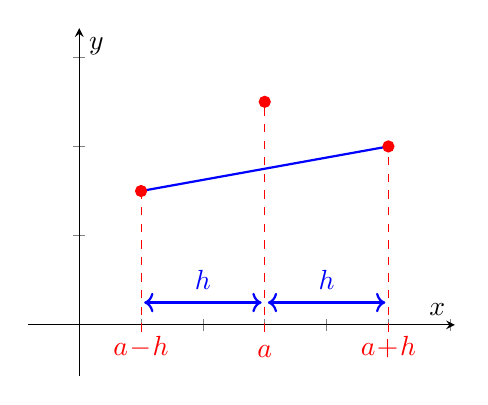
\begin{tikzpicture}
    \begin{axis}[
        legend pos=south east,
        axis x line=middle,
        axis y line=middle,
	xticklabels=\empty,
	yticklabels= \empty,
        grid = none ,
        width=7cm,
        height=6cm,
        grid style={dashed, gray!1},
        xmin=-0.5,     % start the diagram at this x-coordinate
        xmax=11,    % end   the diagram at this x-coordinate
        ymin=-0.5,     % start the diagram at this y-coordinate
        ymax= 6,   % end   the diagram at this y-coordinate
        xlabel=$x$,
        ylabel=$y$,
        enlargelimits=true,
        tension=0.08]

  \addplot[red, only marks, mark=*] coordinates {(2,3)(6,5)(10,4)};
  \draw [red,dashed] (axis cs: 2,-0.15) -- (axis cs: 2,3);
  \draw [red,dashed] (axis cs: 6,-0.15) -- (axis cs: 6,5);
  \draw [red,dashed] (axis cs: 10,-0.15) -- (axis cs: 10,4);
  \draw[blue,thick](axis cs: 2,3)--(axis cs: 10,4);
  \draw [<->,thick, blue] (axis cs: 2.1,0.5) -- (axis cs: 5.9,0.5);
   \draw [<->,thick, blue] (axis cs: 6.1,0.5) -- (axis cs: 9.9,0.5);
      

	\node(x0)[red] at (axis cs: 2,-0.5){$a \! -\! h$};
	\node(x1)[red] at (axis cs: 6,-0.6){$a$};
	\node(x2)[red] at (axis cs: 10,-0.5){$a \! +\! h$};
	\node(h1)[blue] at (axis cs: 4, 1){$h$};
	\node(h2)[blue] at (axis cs: 8, 1){$h$};
    \end{axis}
\end{tikzpicture}
\end{center}

	\noindent Then, averaging the forward and backward distance leads to:
	
\begin{center}
	\LARGE $\frac{\frac{f(a+h)-f(a)}{h} + \frac{\textcolor{red}{-}f(a-h)\textcolor{red}{+}f(a)}{\textcolor{red}{+}h}}{2}$
	\\
	\bigskip
	\normalsize{\textbf{Centered Difference}}\\
	\medskip
	\Large$= \frac{f(a+h) - f(a-h)}{2h}$
	
\end{center}

	\noindent This is the slope of the linear interpolation of the two neighboring points.
	
\begin{center}
	\Large$= \frac{f(a+h) - f(a-h)}{2h}$\\
	\bigskip
	$= \frac{\big( \cancel{f(a)} + f^\prime(a)\cdot h  + \cancel{\frac{f^{\prime \prime}(a)    }{2!}h^2} + \frac{f^{\prime \prime \prime}(a)}{3!}h^3 + ... \big) - \big( \cancel{f(a)} +   f^\prime(a)(-h) +  \cancel{\frac{f^{\prime \prime}(a)}{2!}(-h)^2} +... \big)     }{2h}$\\
	\bigskip
	\large $= \frac{1}{2h} \big(2f^\prime(a) \cdot h + \frac{f^{\prime \prime \prime}(a)}{3!} h^3 + ... \big) = \underbrace{f^\prime(a)}_{\text{wanted}} + \underbrace{\!\!\!\!\!\!\!\!\!\!\!\!\!\!\!\!\!\!\!\!\!\!\!\!\!\!\! \overbrace{\frac{f^{\prime \prime \prime}(a)}{3!}h^2}^{{\text{Dominating term now dependent upon}\, h^2}} \!\!\!\!\!\!\!\!\!\!\!\!\!\!\!\!\!\!\!\!\!\!\!\!\!\!\!           +...}_{\text{truncation error}}$
\end{center}
	
%INSERT Centered Difference Comparison here-------------------------------------------------------------------------------------------
%------------------------------------------------------------------------------------------------------------------------------------------------

\begin{figure}[!htb]
	\center{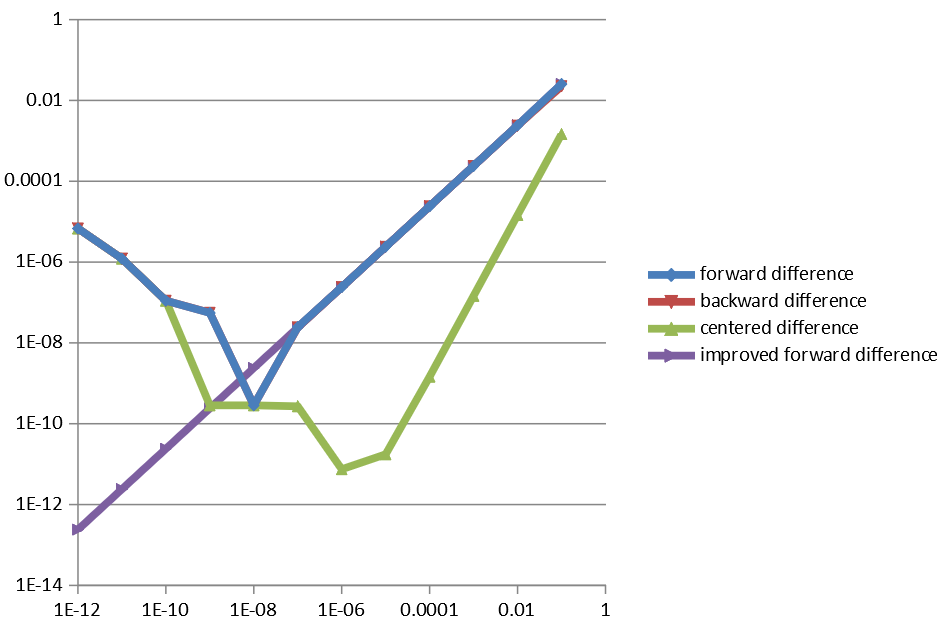
\includegraphics[width=0.8\linewidth]{ExcelDifference2.png}}

	\caption{Round-off error vs stepsize h for $f(x) = \sin x$ }\label{fig:Excel Difference}
\end{figure}
\FloatBarrier


%------------------------------------------------------------------------------------------------------------------------------------------------
%------------------------------------------------------------------------------------------------------------------------------------------------

	\noindent For the centered difference formula, the truncation error is dominated by $constant\cdot h^2$.  Reducing the step size by a factor of 10 reduces error by a factor of 100.  \textit{This is a second-order approximation method.}\\
	
\underline{\textit{Side Remark}}: The Excel experiments showed round-off errors for small step sizes because the difference formulas involve a subtraction of nearly equal numbers.

\begin{center}
	\textbf{Example:} Forward Difference: \qquad \Large $\frac{\sin(a+h) - \sin a}{h}$
\end{center}

	\noindent How can we avoid this?
	
\begin{center}
	$\sin (x+y) - \sin (x-y) = \sin x \cos y + \sin y \cos x - \big( \sin x \cos(-y) + \sin(-y) \cos x \big)$\\
	\bigskip
	$= \cancel{\sin x \cos y} + \sin y \cos x - \big( \cancel{ \sin x \cos y } - \sin y \cos x \big)$\\
	\bigskip
	$= 2 \sin y \cdot \cos x$\\
\end{center}
	
	\noindent We need:

\begin{center}
	\vspace{-5mm}
	$x+y = a + h$\\
	$x-y = a$\\
	\medskip
\end{center}

	\noindent Adding:
	
\begin{center}
	\vspace{-5mm}
	$2x = 2a+h \Leftrightarrow x = a + \frac{h}{2}$\\
	\medskip
\end{center}
	
	\noindent Subtracting:
	
\begin{center}
	\vspace{-5mm}
	$2y = h \Leftrightarrow y = \frac{h}{2}$\\
	\medskip
\end{center}

	\noindent We find:
	
\begin{center}
		\vspace{-5mm}
		$\sin (a+h) - sin (a) = 2 \sin \frac{h}{2} \cdot \big( a + \frac{h}{2} \big)$\\
		\medskip
\end{center}

	\noindent \underline{Excel Results}: We no longer see \textit{any} round-off error, using the product formula instead of subtraction.\\
	
	How can we find \textbf{finite difference} formulas that fit the given problem?\\
	
	\noindent Use quadratic interpolation for three points.

\begin{multicols}{2}
\begin{center}
\begin{tikzpicture}
    \begin{axis}[
        legend pos=south east,
        axis x line=middle,
        axis y line=middle,
	every axis x label/.style={at={(current axis.right of origin)},anchor=north},
	every axis y label/.style={at={(current axis.above origin)},anchor=east},
	xticklabels=\empty,
	yticklabels=\empty
        grid = none ,
        width=9cm,
        height=6cm,
        grid style={dashed, gray!1},
        xmin=-0.15,     % start the diagram at this x-coordinate
        xmax= 4,    % end   the diagram at this x-coordinate
        ymin=-0.1,     % start the diagram at this y-coordinate
        ymax= 1.3,   % end   the diagram at this y-coordinate
        xlabel=$x$,
        ylabel=$y$,
        enlargelimits=true,
        tension=0.08]
        \addplot[domain=-0.25:3.75, blue, thick,samples=250] {-1/8*(x-2.5)^2 +1}; % Parabola

	\addplot[dashed,red,mark=none] coordinates{(0.75,-0.05)(0.75,0.6171875)} node[above left, pos=1] {\footnotesize{$f(a \! - \! h) \!\!\!\!$}}; %x0
	\addplot[dashed,red,mark=none] coordinates{(2,-0.05)(2,0.96875)} node[above, pos=1] {\footnotesize{$f(a)$}}; %x0
	\addplot[dashed,red,mark=none] coordinates{(3.25,-0.05)(3.25,0.9296875)} node[above right, pos=1] {\footnotesize{$f(a \! + \! h)$}}; %x0
	\addplot[red,mark=none] coordinates{(0.75,-0.05)} node[below, pos=0] {$a-h$}; %x1
	\addplot[red,mark=none] coordinates{(2,-0.1)} node[below, pos=0] {$a$}; %x2
	\addplot[red,mark=none] coordinates{(3.25,-0.05)} node[below, pos=0] {$a+h$}; %x2

	\addplot[red, only marks, mark=*] coordinates {(0.75,0.6171875)(2,0.96875)(3.25,0.9296875)};
    \end{axis}
\end{tikzpicture}
\end{center}

	\center \underline{Interpolating parabola}:


\begin{flushright}
	\vspace{-5mm}
	$p(x) = f(a-h)$ \large $\!\! \frac{\big( x-a \big) \big( x-(a+h) \big)}{\big(a-h-a \big) \big( a-h-(a+h) \big)}$\\
 	\medskip
 	\normalsize $ + f(a)$  \large $\!\! \frac{\big( x-(a-h) \big) \big( x-(a+h) \big)}{ a- \big( a-h \big)  \big( a-(a+h) \big)}$\\
 	\medskip
 	\normalsize $+ f(a+h)$ \large $\!\! \frac{\big( x-(a-h) \big) \big( x-a \big)}{\big( a+h - (a-h) \big) \big( (a+h) -a \big)}$

\end{flushright}
\end{multicols}

\vspace{5mm}

\begin{center}
	\normalsize $=f(f-h)$ \large $\frac{ x^2-(2a+h)x + a(a+h) }{ -h(-2h) }$ \normalsize $f(a)$ \large $\frac{(x-a)^2-h^2}{h \cdot (-h)}$ \normalsize $+ f(a+h)$ \large $\!\! \frac{x^2-(2a-h)x + a(a-h) }{ 2h \dot h}$
\end{center}
	
	\noindent Then $p^\prime (x) =$
	
\begin{center}
\vspace{-3mm}
	$f(a-h)$ \large $\!\! \frac{2x - (2a+h)}{2h^2}$ \normalsize $+ \, f(a)$ \large $\!\! \frac{2x-2a}{-h^2}$ \normalsize $+ \, f(a+h)$ \large $\!\! \frac{2x - (2a-h)}{2h^2}$
\end{center}

	\noindent What is happening at $a$?
	
\begin{center}
\vspace{-3mm}
	$p^\prime(a)= f(a-h)$ \large $\!\! \frac{- \cancel{h}}{2h^{\cancel{2}}}$ \normalsize $+ \, \cancel {f(a) \cdot 0} + f(a+h)$
	\large $\!\!\frac{\cancel{h}}{2h^{\cancel{2}}}$
	\normalsize $=\underbrace{   \frac{f(a+h) - f(a-h)}{2h} }_{\text{Centered Difference Formula}} $
\end{center}
	
	\noindent  \underline{We learn}: To find a second order finite difference approximation use an interpolating parabola.
	
\section{Another Way of Creating Formulas:}

	\textit{\Large{ Use Taylor Series}}\\
	
	\begin{multicols}{2}
	
	\begin{tikzpicture}
    \begin{axis}[
        legend pos=south east,
        axis x line=middle,
        axis y line=middle,
	xticklabels=\empty,
	yticklabels= \empty,
        grid = none ,
        width=7cm,
        height=6cm,
        grid style={dashed, gray!1},
        xmin=-2,     % start the diagram at this x-coordinate
        xmax=11,    % end   the diagram at this x-coordinate
        ymin=-1,     % start the diagram at this y-coordinate
        ymax= 6,   % end   the diagram at this y-coordinate
        xlabel=$x$,
        ylabel=$y$,
        enlargelimits=true,
        tension=0.08]

 
  \draw [red,dashed] (axis cs: 2,-0.15) -- (axis cs: 2,.6);
  \draw [red,dashed] (axis cs: 6,-0.15) -- (axis cs: 6,.6);
  \draw [red,dashed] (axis cs: 10,-0.15) -- (axis cs: 10,.6);
  \draw [<->,thick, gray] (axis cs: 2.1,0.5) -- (axis cs: 5.9,0.5);
   \draw [<->,thick, gray] (axis cs: 6.1,0.5) -- (axis cs: 9.9,0.5);
      

	\node(x0)[red] at (axis cs: 2,-0.5){$a$};
	\node(x1)[red] at (axis cs: 6,-0.5){$a \! +\! h$};
	\node(x2)[red] at (axis cs: 10,-0.5){$a \! +\! 2h$};
	\node(h1)[gray] at (axis cs: 4, 1){$h$};
	\node(h2)[gray] at (axis cs: 8, 1){$h$};
    \end{axis}
\end{tikzpicture}
	
	\vspace{5mm}
		\noindent Find a second order formula for the derivative at $a$ when $\big(a, f(a) \big), \big(a+ h, f(a+h) \big), \big(a+2h, f(a+ 2h) \big)$
		are given.  Derivative at left end point.
	\end{multicols}
	
\begin{center}
	$f(a+h) = f(a) + f^\prime (a)h \; +$ \large $\frac{f^{\prime \prime}(a)}{2!}$ \normalsize $\!\! h^2 \;
	+ $ \large $\frac{f^{\prime \prime \prime}(a)}{3!}$ \normalsize $\! \! h^3 + ...$\\
	
	\bigskip
	
	$f(a+2h)= f(a) + f^\prime \cdot 2h + $ \large $ \frac{ f^{\prime \prime}(a) }{ 2! } $ \normalsize $\!\! 4h^2 +  $ \large $ \frac{f^{\prime \prime \prime}(a)}{3!} $ \normalsize $\!\! 8h^3 + ... $
\end{center}

	\noindent Structure of finite difference formula:
	
\begin{center}
	$f^\prime (a) \approx A \cdot f(a) + B \cdot  f(a+h) + C \cdot f(a+2h) $\\
	\bigskip
	$f^ \prime (a) \approx A \cdot f(a) + B \! \cdot \! f(a) + B \! \cdot \! f^\prime (a)h +B$ \large $\! \! \frac{f^{\prime \prime}(a)}{2} $
	\normalsize $h^2  + B$ \large $ \frac{ f^{\prime \prime \prime}(a)}{3!}$ \large $h^3$\\
	\medskip
	$+ C \cdot f(a) + C \cdot f^\prime (a)2h + C$\large $\frac{f^{\prime \prime}(a)}{2}$ \normalsize $4h^2 + C$
	\large $ \frac{ f^{\prime \prime \prime}(a)}{3!} $ \normalsize $\!\! 8h^3$
\end{center}

	\noindent What do we want?

\begin{tabbing}
	\hspace{4cm} \= $A + B + C = 0$ \hspace{5mm} \= to get rid of $f(a)$\\ \\
	\medskip
	\> $hB + 2hC =1$ \> to get $f^\prime(a)$\\ \\
	\>$\frac{B}{2}h^2 + \frac{C}{2}4h^2=0$ \> to get rid of $f^{\prime \prime(a)} \, \leftarrow$ \textit{truncation error}
\end{tabbing}

\vspace{5mm}

\begin{multicols}{2}	
\begin{center}
\begin{tabular}{ccc|l}
	$A$  &  $B$  &  $C$  &  $r.h.s.$\\
	\hline
	1 & 1 & 1 & 0 I\\
	0 & 1 & 2 & $\frac{1}{h}$ II\\
	0 & 1 & 4 & 0 III - II\\
	\hline
	1 & 1 & 1 & 0\\
	0 & 1 & 2 & $\frac{1}{h}$ \\
	0 & 0 & 2 & $\frac{-1}{h}$
\end{tabular}
\end{center}

	\noindent \underline{\textit{Back Substitute}}\\
	$C = \frac{-1}{2h}$\\
	\\
	Plug into II:\\
	$B = \frac{1}{h}-2 \big( \frac{-1}{2h} \big)= \frac{2}{h}$\\
	\\
	Plug into I: \\
	$A = -B - C = \frac{-2}{h} + \frac{1}{2h} = \frac{-4}{2h} + \frac{1}{2h}=\frac{-3}{2h}$
\end{multicols}
	
	\noindent We obtain:
	
\begin{center}
	\vspace{-3mm}
	$f^\prime(a) \approx$ \large $\frac{-3}{2h}$ \normalsize $\!\!\! f(a) \, +$
	\large $\frac{4}{2h}$ \normalsize $\!\!\! f(a \! + \! h) \, -$
	\large $\frac{1}{2h}$ \normalsize $\!\!\! f(a \! + \! 2h)$\\
	\bigskip
	\Large $= \frac{ -3f(a) + 4f(a +  h) - f(a +2h)}{2h}$
\end{center}

\chapter{Numerical Integration}

\begin{center}
\fbox
{
	\parbox{0.6\textwidth}
	{
		\textbf{\underline{Fundamental Theorem of Calculus}:}\\
		If $f$ is continuous on $[a,b]$ then
		\begin{center}
		\vspace{-1cm}
			$$\int_{a}^{b}f(x) dx = F(b) - F(a)$$
		\end{center}
		where $F$ is any anti-derivative of $f$.
	}
}
\end{center}

	\noindent \textit{\underline{Problem}:} It may be difficult to find an anti-derivative or even impossible to write as a finite
	 combination of ``basic functions''.  (Power series may help using infinite combinations but not all functions possess
	 power series representation.)\\
	 
	 Another motivation: How do we integrate when the function is only known by some sample values?\\
	 
\begin{multicols}{2}

\begin{tikzpicture}
    \begin{axis}[
        legend pos=south east,
        axis x line=middle,
        axis y line=middle,
	xticklabels=\empty,
	yticklabels= \empty,
        grid = none ,
        width=7cm,
        height=6cm,
        grid style={dashed, gray!1},
        xmin=-2,     % start the diagram at this x-coordinate
        xmax=19,    % end   the diagram at this x-coordinate
        ymin=-1,     % start the diagram at this y-coordinate
        ymax= 6,   % end   the diagram at this y-coordinate
        xlabel=$x$,
        ylabel=$y$,
        enlargelimits=true,
        tension=0.08]

  \addplot[red, only marks, mark=*] coordinates {(2,5)(8,3)(13,4)(18,2)};
  \draw [red,dashed] (axis cs: 2,-0.15) -- (axis cs: 2,.6);
  \draw [red,dashed] (axis cs: 18,-0.15) -- (axis cs: 18,.6);
      
	\node(a)[red] at (axis cs: 2,-0.5){$a$};
	\node(b)[red] at (axis cs: 18,-0.5){$b$};
    \end{axis}
\end{tikzpicture}


	\Large $$\!\!\!\!\!\!\!\! \int_{a}^{b} f(x)dx =  \text{?}$$
	
	\normalsize
\end{multicols}

	\noindent \textit{\underline{Already expected}:} Use polynomial interpolation or piecewise polynomial interpolation
	(to avoid large oscillations).\\
	
	First let's consider the definition of the definite integral as limit of the Riemann Sums:


\begin{multicols}{2}
\begin{center}
\fbox
{
	\parbox{0.5\textwidth}
	{
		\textbf{\underline{Riemann Sum}}\\

		\begin{center}
		\vspace{-1.5cm}
			$$\int_{a}^{b}f(x) dx =\lim\limits_{n\to \infty} \sum_{i=1}^{n} f(x_i^*) \cdot \frac{b-a}{n}$$
		\end{center}

	}
}

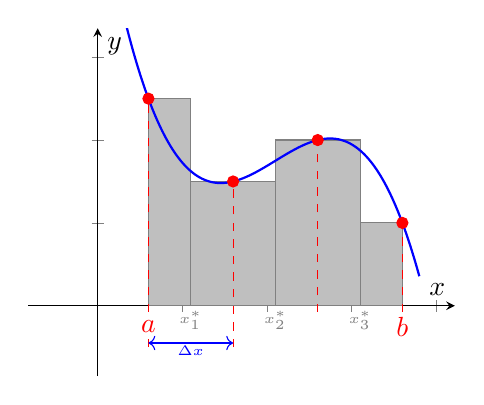
\begin{tikzpicture}
    \begin{axis}[
        legend pos=south east,
        axis x line=middle,
        axis y line=middle,
	xticklabels=\empty,
	yticklabels= \empty,
        grid = none ,
        width=7cm,
        height=6cm,
        grid style={dashed, gray!1},
        xmin=-2,     % start the diagram at this x-coordinate
        xmax=19,    % end   the diagram at this x-coordinate
        ymin=-1,     % start the diagram at this y-coordinate
        ymax= 6,   % end   the diagram at this y-coordinate
        xlabel=$x$,
        ylabel=$y$,
        enlargelimits=true,
        tension=0.08]

\filldraw[fill=lightgray, draw=gray] (axis cs: 3,0) rectangle (axis cs: 5.5,5);
\filldraw[fill=lightgray, draw=gray] (axis cs: 5.5,0) rectangle (axis cs: 10.5,3);
\filldraw[fill=lightgray, draw=gray] (axis cs: 10.5,0) rectangle (axis cs: 15.5,4);
\filldraw[fill=lightgray, draw=gray] (axis cs: 15.5,0) rectangle (axis cs: 18,2);


 \addplot[domain=1.25:19, blue, thick,samples=250] {-1/150*(x-8)*(x-13)*(x-18)+3/250*(x-3)*(x-13)*(x-18)-2/125*(x-3)*(x-8)*(x-18)+1/375*(x-3)*(x-8)*(x-13)}; % Parabola
  \addplot[red, only marks, mark=*] coordinates {(3,5)(8,3)(13,4)(18,2)};
  \draw [red,dashed] (axis cs: 3,-0.15) -- (axis cs: 3,5);
    \draw [red,dashed] (axis cs: 8,-1) -- (axis cs: 8,3);
     \draw [red,dashed] (axis cs: 13,-0.15) -- (axis cs: 13,4);
  \draw [red,dashed] (axis cs: 18,-0.15) -- (axis cs: 18,2);
  \draw [red,dashed] (axis cs: 3,-1) -- (axis cs: 3,-0.7);
  
    \draw [<->, blue] (axis cs: 3,-0.9) -- (axis cs: 8,-0.9);
  
  
	\node(a)[red] at (axis cs: 3,-0.5){$a$};
	\node(xd)[blue] at (axis cs: 5.5,-1.1){\tiny{$\Delta x$}};
	\node(x1)[gray] at (axis cs: 5.5,-0.35){\tiny{$x_1^*$}};
	\node(x2)[gray] at (axis cs: 10.5,-0.35){\tiny{$x_2^*$}};
	\node(x3)[gray] at (axis cs: 15.5,-0.35){\tiny{$x_3^*$}};
	\node(b)[red] at (axis cs: 18,-0.5){$b$};
    \end{axis}
\end{tikzpicture}
\end{center}
\end{multicols}
	\noindent We obtain an approximation of the definite integral using a Riemann Sum:
	
\begin{center}
	$$\int_{a}^{b}f(x) dx \approx \sum_{i=1}^{n} f(x_i^*) \cdot \frac{b-a}{n}$$
\end{center}
	
\section{Midpoint Rule}
\begin{multicols}{2}
	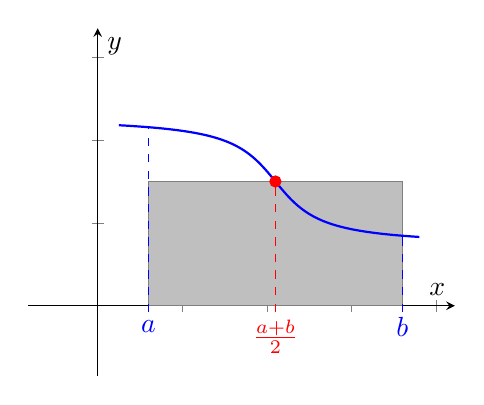
\begin{tikzpicture}
    \begin{axis}[
        legend pos=south east,
        axis x line=middle,
        axis y line=middle,
	xticklabels=\empty,
	yticklabels= \empty,
        grid = none ,
        width=7cm,
        height=6cm,
        grid style={dashed, gray!1},
        xmin=-2,     % start the diagram at this x-coordinate
        xmax=19,    % end   the diagram at this x-coordinate
        ymin=-1,     % start the diagram at this y-coordinate
        ymax= 6,   % end   the diagram at this y-coordinate
        xlabel=$x$,
        ylabel=$y$,
        enlargelimits=true,
        tension=0.08]

\filldraw[fill=lightgray, draw=gray] (axis cs: 3,0) rectangle (axis cs: 18,3);


 \addplot[domain=1.25:19, blue, thick,samples=250] {rad(-atan(x/2-5.25))+3}; % Parabola
  \addplot[red, only marks, mark=*] coordinates {(10.5,3)};
  \draw [blue,dashed] (axis cs: 3,-0.15) -- (axis cs: 3,4.31);
     \draw [red,dashed] (axis cs: 10.5,-0.15) -- (axis cs: 10.5,3);
  \draw [blue,dashed] (axis cs: 18,-0.15) -- (axis cs: 18,1.68);
  

	\node(a)[blue] at (axis cs: 3,-0.5){$a$};
	\node(b)[blue] at (axis cs: 18,-0.5){$b$};
	\node(MP)[red] at (axis cs: 10.5,-0.75){$\frac{a+b}{2}$};
    \end{axis}
\end{tikzpicture}

\begin{center}
	$$\int_{a}^{b}f(x) dx \approx
	\underbrace{\underbrace{f \big( \frac{a+b}{2} \big)}_{\text{height}} \cdot \underbrace{(b-a)}_{\text{width}}}_{\text{area of rectangle}}$$
\end{center}
\end{multicols}
\bigskip

	\noindent \textbf{Example:}

\vspace{-1cm}	
\begin{center}
	$$  \int_{0}^{1} e^{-x^2}dx \quad \approx \quad e^{-(\frac{1}{2})^2}\cdot (1-0) \quad = \quad 0.77...$$
\end{center}

	\noindent Is this approximation any good?
	
\begin{center}
	\begin{tikzpicture}
    \begin{axis}[
        legend pos=south east,
        axis x line=middle,
        axis y line=middle,
	xticklabels=\empty,
	yticklabels= \empty,
        grid = none ,
        width=7cm,
        height=6cm,
        grid style={dashed, gray!1},
        xmin=-0.15,     % start the diagram at this x-coordinate
        xmax=1.15,    % end   the diagram at this x-coordinate
        ymin=-0.15,     % start the diagram at this y-coordinate
        ymax= 1.15,   % end   the diagram at this y-coordinate
        xlabel=$x$,
        ylabel=$y$,
        enlargelimits=true,
        tension=0.08]

\filldraw[fill=lightgray, draw=gray] (axis cs: 3,0) rectangle (axis cs: 18,3);


 \addplot[domain=0:1, blue, thick,samples=250] {exp(-x^2)}; % Parabola
  \addplot[red, only marks, mark=*] coordinates {(10.5,3)};
  \draw [red,dashed] (axis cs: 1,-0.05) -- (axis cs: 1,1.15);

  \draw [red,dashed] (axis cs: -0.05,1) -- (axis cs: 1.15,1);
  

	\node(a)[red] at (axis cs: -0.1,1){1};
	\node(b)[red] at (axis cs: 1,-0.15){1};
	\node(MP)[blue] at (axis cs: 0.35,1.15){\large{$y=e^{-x^2}$}};
    \end{axis}
\end{tikzpicture}
\end{center}
\bigskip
	\noindent For more accuracy use the midpoint rule repeatedly.

\begin{multicols}{2}	
\begin{center}
	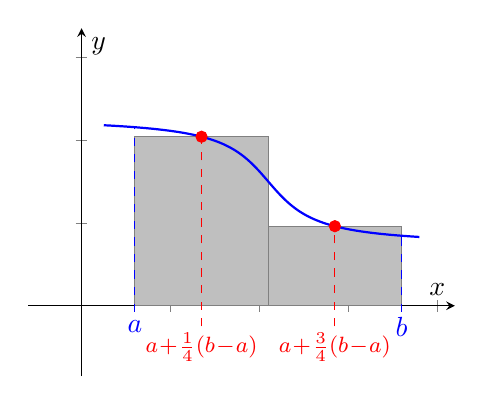
\begin{tikzpicture}
    \begin{axis}[
        legend pos=south east,
        axis x line=middle,
        axis y line=middle,
	xticklabels=\empty,
	yticklabels= \empty,
        grid = none ,
        width=7cm,
        height=6cm,
        grid style={dashed, gray!1},
        xmin=-1,     % start the diagram at this x-coordinate
        xmax=19,    % end   the diagram at this x-coordinate
        ymin=-1,     % start the diagram at this y-coordinate
        ymax= 6,   % end   the diagram at this y-coordinate
        xlabel=$x$,
        ylabel=$y$,
        enlargelimits=true,
        tension=0.08]

\filldraw[fill=lightgray, draw=gray] (axis cs: 3,0) rectangle (axis cs: 10.5,4.08);
\filldraw[fill=lightgray, draw=gray] (axis cs: 10.5,0) rectangle (axis cs: 18,1.92);


 \addplot[domain=1.25:19, blue, thick,samples=250] {rad(-atan(x/2-5.25))+3}; % Parabola
  \addplot[red, only marks, mark=*] coordinates {(6.75,4.08)(14.25,1.92)};
  \draw [blue,dashed] (axis cs: 3,-0.15) -- (axis cs: 3,4.31);
     \draw [red,dashed] (axis cs: 6.75,-0.5) -- (axis cs: 6.75,4.08);
      \draw [red,dashed] (axis cs: 14.25,-0.5) -- (axis cs: 14.25,1.92);
  \draw [blue,dashed] (axis cs: 18,-0.15) -- (axis cs: 18,1.68);
  

	\node(a)[blue] at (axis cs: 3,-0.5){$a$};
	\node(b)[blue] at (axis cs: 18,-0.5){$b$};
	\node(MP1)[red] at (axis cs: 6.75,-1){\footnotesize{$a\!+\! \frac{1}{4}(b\!-\!a)$}};
	\node(MP2)[red] at (axis cs: 14.25,-1){\footnotesize{$a\!+\! \frac{3}{4}(b\!-\!a)$}};
    \end{axis}
\end{tikzpicture}
\normalsize
	$M_2 \! =\! f\big( a \!+\! \frac{1}{4}(b-a) \big) \frac{b\!-\!a}{2}  + f\big( a \!+\! \frac{3}{4}(b\!-\!a) \big) \frac{b-a}{2}$\\
	\bigskip
	$= \frac{b-a}{2} \Big[ f \big(a + \frac{1}{4}(b-a)\big) + f \big(a + \frac{3}{4}(b-a)\big) \Big]$

\end{center}
\end{multicols}

	\noindent  Back to our example:
	
\begin{center}
\vspace{-3mm}
	$M_2 = \frac{1}{2} \big( e^{-(\frac{1}{4})^2}+  e^{-(\frac{3}{4})^2} \big) \approx 0.7545$\\

\bigskip

\fbox
{
	\parbox{0.6\textwidth}
	{
		\noindent \textit{\underline{Simple approach}:}\\
		\vspace{-3mm}
		\\
		Compute $M_1, \, M_2, \, M_4, \, M_8, ...$ until $M_n \! \approx \! M_{2n}$ within our desired tolerance. Then:

		\begin{center}
		\vspace{-1cm}
			$$\int_{a}^{b}f(x) dx \, \approx \, M_{2n}$$
		\end{center}
	}
}
\end{center}

	\noindent \textit{\underline{Be aware}:} With an increasing number of intervals, the summands become smaller and more
	susceptible to round-off errors. They may add up to create a huge uncertainty.
	
\section{Trapezoid Rule}

\begin{center}
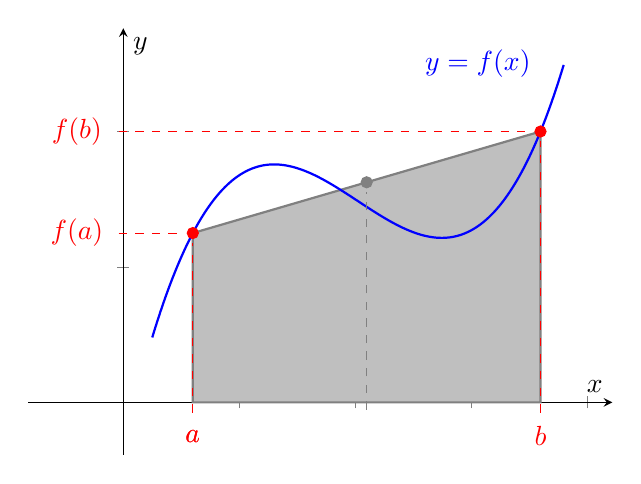
\begin{tikzpicture}
    \begin{axis}[
        legend pos=south east,
        axis x line=middle,
        axis y line=middle,
	xticklabels=\empty,
	yticklabels= \empty,
        grid = none ,
        width=9cm,
        height=7cm,
        grid style={dashed, gray!1},
        xmin=-2,     % start the diagram at this x-coordinate
        xmax=19,    % end   the diagram at this x-coordinate
        ymin=-0.25,     % start the diagram at this y-coordinate
        ymax= 5,   % end   the diagram at this y-coordinate
        xlabel=$x$,
        ylabel=$y$,
        enlargelimits=true,
        tension=0.08]
        
        \node(A1) at (axis cs: 3, 0){};
        \node(A2) at (axis cs: 3, 2.5){};
       \node(B1) at (axis cs: 18, 0){};        
        \node(B2) at (axis cs: 18, 4){};
         \node(MP1) at (axis cs: 10.5,-0.25){};
         \node(MP2) at (axis cs: 10.5,3.25){};

\draw[draw = gray, thick,  fill = lightgray] (A1.center) -- (A2.center) -- (B2.center) -- (B1.center) -- cycle;
  \addplot[domain=1.25:19, blue, thick,samples=250] {(x-7)*(x-10)*(x-18)/(-840)+(x-3)*(x-10)*(x-18)/88+(x-3)*(x-7)*(x-18)/(-168)+(x-3)*(x-7)*(x-10)/660 +2}; % Function
  \addplot[red, only marks, mark=*] coordinates {(3,2.5)(18,4)};
  \addplot[gray, only marks, mark=*] coordinates{(10.5,3.25)};
  \draw [red,dashed] (axis cs: 3,-0.15) -- (A2);
    \draw [red,dashed] (axis cs: -0.2,2.5) -- (A2);
    \draw [red,dashed] (axis cs: -0.2,4) -- (B2);
     \draw [gray,dashed] (MP1) -- (MP2);
  \draw [red,dashed] (axis cs: 18,-0.15) -- (B2);
  

	\node(a)[red] at (axis cs: 3,-0.5){$a$};
	\node(b)[red] at (axis cs: 18,-0.5){$b$};
	\node(fA)[red] at (axis cs: -2,2.5){$f(a)$};
	\node(fB)[red] at (axis cs: -2,4){$f(b)$};
	\node(a)[red] at (axis cs: 3,-0.5){$a$};
	\node(yf)[blue] at (axis cs: 15.3,5){$y=f(x)$};
    \end{axis}
\end{tikzpicture}
\end{center}

	
	Use linear interpolation between the end points:

\begin{center}
	$T_1 =$\large$ \frac{f(a)+f(b)}{2}$\normalsize$ (b-a)$\\
\end{center}
\bigskip
\begin{multicols}{2}
\begin{center}

	\textbf{\underline{Piecewise Linear Interpolation}}\\
	\bigskip

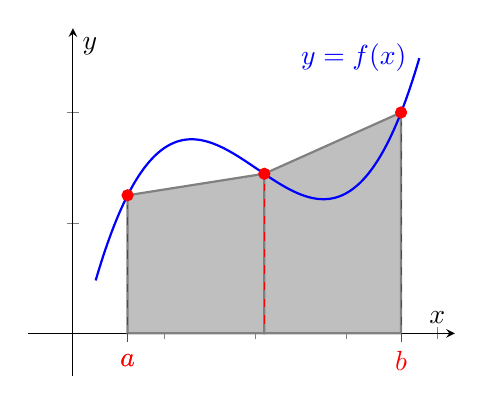
\begin{tikzpicture}
    \begin{axis}[
        legend pos=south east,
        axis x line=middle,
        axis y line=middle,
	xticklabels=\empty,
	yticklabels= \empty,
        grid = none ,
        width=7cm,
        height=6cm,
        grid style={dashed, gray!1},
        xmin=-0.5,     % start the diagram at this x-coordinate
        xmax=19,    % end   the diagram at this x-coordinate
        ymin=-0.25,     % start the diagram at this y-coordinate
        ymax= 5,   % end   the diagram at this y-coordinate
        xlabel=$x$,
        ylabel=$y$,
        enlargelimits=true,
        tension=0.08]
        
        \node(A1) at (axis cs: 3, 0){};
        \node(A2) at (axis cs: 3, 2.5){};
       \node(B1) at (axis cs: 18, 0){};        
        \node(B2) at (axis cs: 18, 4){};
         \node(MP1) at (axis cs: 10.5,0){};
         \node(MP2) at (axis cs: 10.5,2.89){};

\draw[draw = gray, thick,  fill = lightgray] (A1.center) -- (A2.center) -- (MP2.center) -- (MP1.center) -- cycle;
\draw[draw = gray, thick,  fill = lightgray] (MP1.center) -- (MP2.center) -- (B2.center) -- (B1.center) -- cycle;
  \addplot[domain=1.25:19, blue, thick,samples=250] {(x-7)*(x-10)*(x-18)/(-840)+(x-3)*(x-10)*(x-18)/88+(x-3)*(x-7)*(x-18)/(-168)+(x-3)*(x-7)*(x-10)/660 +2}; % Function
  \addplot[red, only marks, mark=*] coordinates {(3,2.5)(10.5,2.89)(18,4)};
  \draw [red,dashed] (axis cs: 3,-0.15) -- (A2);
  \draw [red,dashed] (MP1) -- (MP2);
  \draw [red,dashed] (axis cs: 18,-0.15) -- (B2);
  

	\node(a)[red] at (axis cs: 3,-0.5){$a$};
	\node(b)[red] at (axis cs: 18,-0.5){$b$};
	\node(a)[red] at (axis cs: 3,-0.5){$a$};
	\node(yf)[blue] at (axis cs: 15.4,5){$y=f(x)$};
    \end{axis}
\end{tikzpicture}
\end{center}

	$$\int_{a}^{b}f(x) dx \, \approx T_2 = \frac{f(a)-f(\frac{a+b}{2})}{2}\cdot \frac{b-a}{2}$$\\
	\vspace{-5mm} $$+ \frac{f(\frac{a+b}{2})+f(b)}{2} \cdot \frac{b-a}{2}$$

\end{multicols}

\begin{center}
\vspace{-5mm}
	$$= \Big(  \frac{f(a)}{2} + f\big(\frac{a+b}{2}\big) + \frac{f(b)}{2}  \Big) \cdot  \frac{b-a}{2}
	 \quad = \quad \frac{T_1 + M_1}{2}$$ \\
	 
\pagebreak
\end{center}


\begin{multicols}{2}

	\noindent This pattern continues:\\
	$$ T_4 = \frac{T_2 +M_2}{2} $$\\
	$$ T_8 = \frac{T_4 +M_4}{2} $$\\ \\

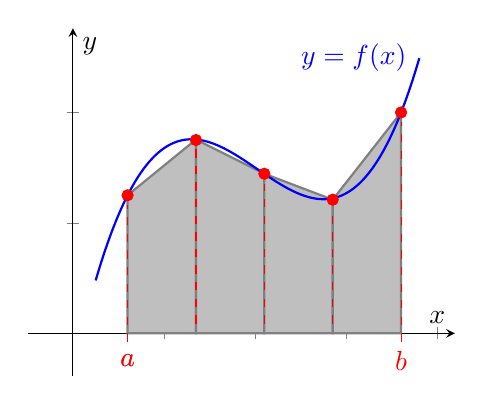
\begin{tikzpicture}
    \begin{axis}[
        legend pos=south east,
        axis x line=middle,
        axis y line=middle,
	xticklabels=\empty,
	yticklabels= \empty,
        grid = none ,
        width=7cm,
        height=6cm,
        grid style={dashed, gray!1},
        xmin=-0.5,     % start the diagram at this x-coordinate
        xmax=19,    % end   the diagram at this x-coordinate
        ymin=-0.25,     % start the diagram at this y-coordinate
        ymax= 5,   % end   the diagram at this y-coordinate
        xlabel=$x$,
        ylabel=$y$,
        enlargelimits=true,
        tension=0.08]
        
        \node(A1) at (axis cs: 3, 0){};
        \node(A2) at (axis cs: 3, 2.5){};
       \node(B1) at (axis cs: 18, 0){};        
        \node(B2) at (axis cs: 18, 4){};
         \node(C1) at (axis cs: 10.5,0){};
         \node(C2) at (axis cs: 10.5,2.89){};
         \node(D1) at (axis cs: 6.75,0){};
         \node(D2) at (axis cs: 6.75,3.51){};
         \node(E1) at (axis cs: 14.25,0){};
         \node(E2) at (axis cs: 14.25,2.42){};

\draw[draw = gray, thick,  fill = lightgray] (A1.center) -- (A2.center) -- (D2.center) -- (D1.center) -- cycle;
\draw[draw = gray, thick,  fill = lightgray] (D1.center) -- (D2.center) -- (C2.center) -- (C1.center) -- cycle;
\draw[draw = gray, thick,  fill = lightgray] (C1.center) -- (C2.center) -- (E2.center) -- (E1.center) -- cycle;
\draw[draw = gray, thick,  fill = lightgray] (E1.center) -- (E2.center) -- (B2.center) -- (B1.center) -- cycle;
  \addplot[domain=1.25:19, blue, thick,samples=250] {(x-7)*(x-10)*(x-18)/(-840)+(x-3)*(x-10)*(x-18)/88+(x-3)*(x-7)*(x-18)/(-168)+(x-3)*(x-7)*(x-10)/660 +2}; % Function
  \addplot[red, only marks, mark=*] coordinates {(3,2.5)(6.75,3.5)(10.5,2.89)(14.25,2.42)(18,4)};
  \draw [red,dashed] (axis cs: 3,-0.15) -- (A2);
  \draw [red,dashed] (C1) -- (C2);
   \draw [red,dashed] (D1) -- (D2);
    \draw [red,dashed] (E1) -- (E2);
  \draw [red,dashed] (axis cs: 18,-0.15) -- (B2);
  

	\node(a)[red] at (axis cs: 3,-0.5){$a$};
	\node(b)[red] at (axis cs: 18,-0.5){$b$};
	\node(a)[red] at (axis cs: 3,-0.5){$a$};
	\node(yf)[blue] at (axis cs: 15.4,5){$y=f(x)$};
    \end{axis}
\end{tikzpicture}
\end{multicols}

	\noindent \textbf{Example:} $\int^1_0 e^{-x^2}dx $ \\
	

	
\begin{multicols}{2}
	


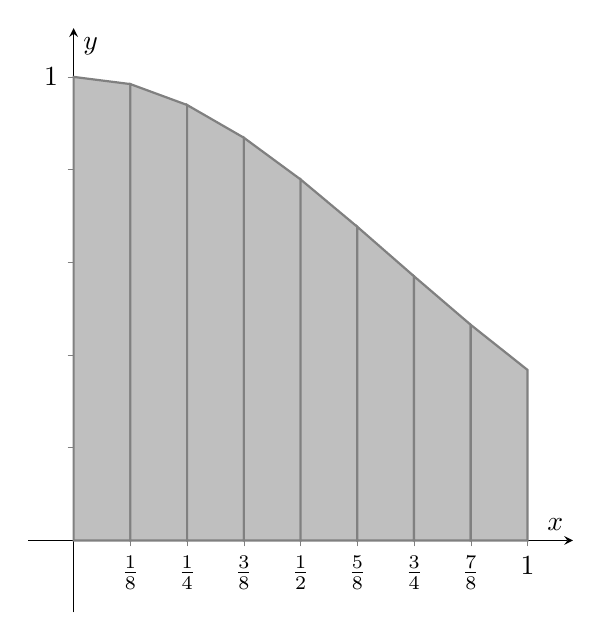
\begin{tikzpicture}
    \begin{axis}[
    xtick={0.125,0.25,...,1 },
        legend pos=south east,
        axis x line=middle,
        axis y line=middle,
	xticklabels={$\frac{1}{8}$, $\frac{1}{4}$,$\frac{3}{8}$,$\frac{1}{2}$,$\frac{5}{8}$,$\frac{3}{4}$,$\frac{7}{8}$,$1$},
	yticklabels= \empty,
        grid = none ,
        width=8.5cm,
        height=9cm,
        grid style={dashed, gray!1},
        xmin=0,     % start the diagram at this x-coordinate
        xmax=1,    % end   the diagram at this x-coordinate
        ymin=-0.05,     % start the diagram at this y-coordinate
        ymax= 1,   % end   the diagram at this y-coordinate
        xlabel=$x$,
        ylabel=$y$,
        enlargelimits=true,
        tension=0.08]
        
        \node(A1) at (axis cs: 0, 0){};
        \node(A2) at (axis cs: 0,1){};
       \node(B1) at (axis cs: 0.125, 0){};        
        \node(B2) at (axis cs: 0.125, 0.9845){};
         \node(C1) at (axis cs: 0.25,0){};
         \node(C2) at (axis cs: 0.25,0.9394){};
         \node(D1) at (axis cs: 0.375,0){};
         \node(D2) at (axis cs: 0.375,0.8688){};
         \node(E1) at (axis cs: 0.5,0){};
         \node(E2) at (axis cs: 0.5,0.7788){};
         \node(F1) at (axis cs: 0.625,0){};
         \node(F2) at (axis cs: 0.625,0.6766){};
         \node(G1) at (axis cs: 0.75,0){};
         \node(G2) at (axis cs: 0.75,0.5698){};
         \node(H1) at (axis cs: 0.875,0){};
         \node(H2) at (axis cs: 0.875,0.4650){};
         \node(I1) at (axis cs: 1,0){};
         \node(I2) at (axis cs: 1,0.3678){};

\draw[draw = gray, thick,  fill = lightgray] (A1.center) -- (A2.center) -- (B2.center) -- (B1.center) -- cycle;
\draw[draw = gray, thick,  fill = lightgray] (B1.center) -- (B2.center) -- (C2.center) -- (C1.center) -- cycle;
\draw[draw = gray, thick,  fill = lightgray] (C1.center) -- (C2.center) -- (D2.center) -- (D1.center) -- cycle;
\draw[draw = gray, thick,  fill = lightgray] (D1.center) -- (D2.center) -- (E2.center) -- (E1.center) -- cycle;
\draw[draw = gray, thick,  fill = lightgray] (E1.center) -- (E2.center) -- (F2.center) -- (F1.center) -- cycle;
\draw[draw = gray, thick,  fill = lightgray] (F1.center) -- (F2.center) -- (G2.center) -- (G1.center) -- cycle;
\draw[draw = gray, thick,  fill = lightgray] (G1.center) -- (G2.center) -- (H2.center) -- (H1.center) -- cycle;
\draw[draw = gray, thick,  fill = lightgray] (H1.center) -- (H2.center) -- (I2.center) -- (I1.center) -- cycle;

	\node(a) at (axis cs: -0.05,1){1};
%	\node(MP)[blue] at (axis cs: 0.5,1){\large{$y=e^{-x^2}$}};
    \end{axis}
\end{tikzpicture}
	\vspace{3cm}

	$$ T_1 = \frac{(e^{-0}+e^{-1})\cdot(1-0)}{2} =  0.6839...$$
	$$M_1 = e^{- (\frac{1}{2})^2} \cdot(1-0) = 0.7788...$$
	$$T_2 = \frac{T_1+M_1}{2}=0.7313...$$
	$$M_2 = \big( e^{-(\frac{1}{4})^2}+e^{-(\frac{3}{4})^2} \big) \cdot \frac{1}{2} = 0.7545...$$
	$$T_4 = \frac{T_2+M_2}{2}=0.7429...$$
	$$M_4 = \Big[  e^{-(\frac{1}{8})^2} +  e^{-(\frac{3}{8})^2} +  e^{-(\frac{5}{8})^2} +  e^{-(\frac{7}{8})^2} \Big] \cdot \frac{1}{4}$$
	$$T_8 = \frac{T_4+M_4}{2}$$

\end{multicols}

	\textbf{Note:} With this procedure, each function value is only computed once.  We can accelerate this process using the
	\textbf{Romberg scheme}.  In our example, we can begin the Romberg scheme by arranging our first four $T$-values in a
	column.  Beginning with $T_2$, we multiply our $T-value$ by 4, then subtract the preceding $T$-value.  We then divide
	our result by 3.

\begin{center}
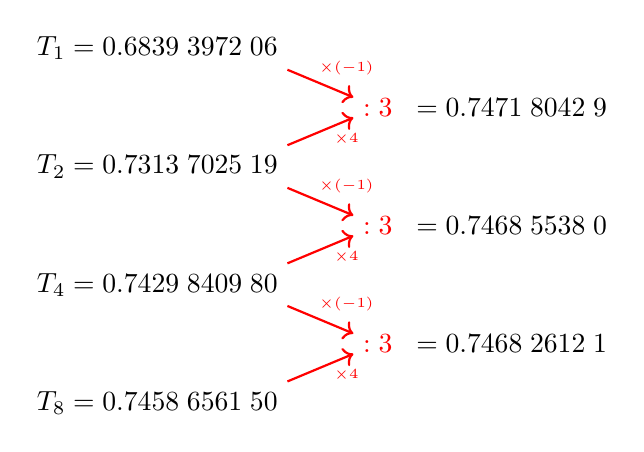
\begin{tikzpicture}

	\node (T1) at (1,5.25) {$T_1 = 0.6839 \; 3972 \; 06$};
	\node (T2) at (1,3.75) {$T_2 = 0.7313 \;7025 \; 19$};
	\node (T4) at (1,2.25) {$T_4 = 0.7429 \; 8409 \; 80$};
	\node (T8) at (1,.75) {$T_8 = 0.7458 \; 6561 \; 50$}; %Some uncertainty about last 2 digits.  Maybe recalculate in MATLAB
	\node (A1)[red] at (3.8, 4.5){$:3$};
	\node (A2)[red] at (3.8, 3){$:3$};
	\node (A3)[red] at (3.8, 1.5){$:3$};
	
	\node (B1) at (5.5,4.5){$= 0.7471\;8042\;9$};
	\node (B2) at (5.5,3){$= 0.7468\;5538\;0$};
	\node (B3) at (5.5,1.5){$= 0.7468\;2612\;1$};
	
	\draw [->, thick,red] (T1.south east) to (A1);
	\draw [->, thick,red] (T2.north east) to (A1);
	\draw [->, thick,red] (T2.south east) to (A2);
	\draw [->, thick,red] (T4.north east) to (A2);
	\draw [->, thick,red] (T4.south east) to (A3);
	\draw [->, thick,red] (T8.north east) to (A3);

	\node (A1a)[red] at (3.4,5){\tiny{$\times (-1)$}};
	\node (A1b)[red] at (3.4,4.1){\tiny{$\times 4$}};
	\node (A2a)[red] at (3.4,3.5){\tiny{$\times (-1)$}};	
	\node (A2b)[red] at (3.4,2.6){\tiny{$\times 4$}};
	\node (A3a)[red] at (3.4,2){\tiny{$\times (-1)$}};	
	\node (A3b)[red] at (3.4,1.1){\tiny{$\times 4$}};

\normalsize
	
\end{tikzpicture}
\end{center}
	\pagebreak

	\noindent We continue this scheme by repeating the process on our results from the second column, only this time, instead of 
	multiplying each new term by 4 and later dividing by 3, we multiply by 16 and divide by 15.  The preceding term still has a
	coefficient of -1.
	
\begin{center}
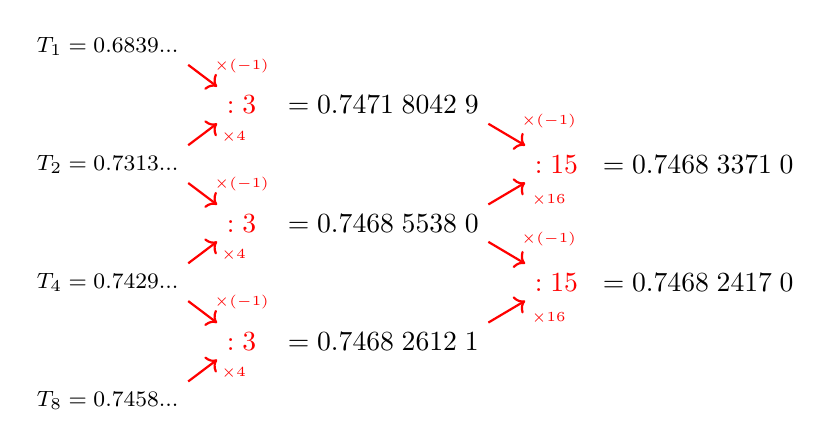
\begin{tikzpicture}

	\node (T1) at (1,5.25) {\footnotesize{$T_1 = 0.6839...$}};
	\node (T2) at (1,3.75) {\footnotesize{$T_2 = 0.7313...$}};
	\node (T4) at (1,2.25) {\footnotesize{$T_4 = 0.7429...$}};
	\node (T8) at (1,.75) {\footnotesize{$T_8 = 0.7458...$}}; %Some uncertainty about last 2 digits.  Maybe recalculate in MATLAB
	\node (A1)[red] at (2.7, 4.5){$:3$};
	\node (A2)[red] at (2.7, 3){$:3$};
	\node (A3)[red] at (2.7, 1.5){$:3$};
	
	\node (B1)at (4.5,4.5){$= 0.7471\;8042\;9$};
	\node (B2) at (4.5,3){$= 0.7468\;5538\;0$};
	\node (B3) at (4.5,1.5){$= 0.7468\;2612\;1$};
	\node (D1)[red] at (6.7, 3.75){$:15$};
	\node (D2)[red] at (6.7, 2.25){$:15$};
	
	\node (E1) at (8.5,3.75){$= 0.7468\;3371\;0$};
	\node (E1) at (8.5,2.25){$= 0.7468\;2417\;0$};
	
%	\node (F1)[red] at (11, 4){$:63$};

	\draw [->, thick,red] (T1.south east) to (A1);
	\draw [->, thick,red] (T2.north east) to (A1);
	\draw [->, thick,red] (T2.south east) to (A2);
	\draw [->, thick,red] (T4.north east) to (A2);
	\draw [->, thick,red] (T4.south east) to (A3);
	\draw [->, thick,red] (T8.north east) to (A3);

	\draw [->, thick,red] (B1.south east) to (D1);
	\draw [->, thick,red] (B2.north east) to (D1);
	\draw [->, thick,red] (B2.south east) to (D2);
	\draw [->, thick,red] (B3.north east) to (D2);

	\node (A1a)[red] at (2.7,5){\tiny{$\times (-1)$}};
	\node (A1b)[red] at (2.6,4.1){\tiny{$\times 4$}};
	\node (A2a)[red] at (2.7,3.5){\tiny{$\times (-1)$}};	
	\node (A2b)[red] at (2.6,2.6){\tiny{$\times 4$}};
	\node (A3a)[red] at (2.7,2){\tiny{$\times (-1)$}};	
	\node (A3b)[red] at (2.6,1.1){\tiny{$\times 4$}};

	\node (D1a)[red] at (6.6,4.3){\tiny{$\times (-1)$}};
	\node (D1b)[red] at (6.6,3.3){\tiny{$\times 16$}};
	\node (D2a)[red] at (6.6,2.8){\tiny{$\times (-1)$}};
	\node (D2b)[red] at (6.6,1.8){\tiny{$\times 16$}};	
	
\normalsize
	
\end{tikzpicture}
\end{center}

	In the third iteration of our example, we multiply our lower column value by 64, subtract the upper value, then divide the result 
	by 63.  At this point we notice the pattern that each subsequent column is multiplied by a progressively higher power of 4.  In
	 the first column we multiplied our terms by $4^1$ and then divided by 3 (i.e. $4^1-1$).  In the next column we multiply by 
	 $4^2$ and divide by $4^2-1$.
	 
\begin{center}

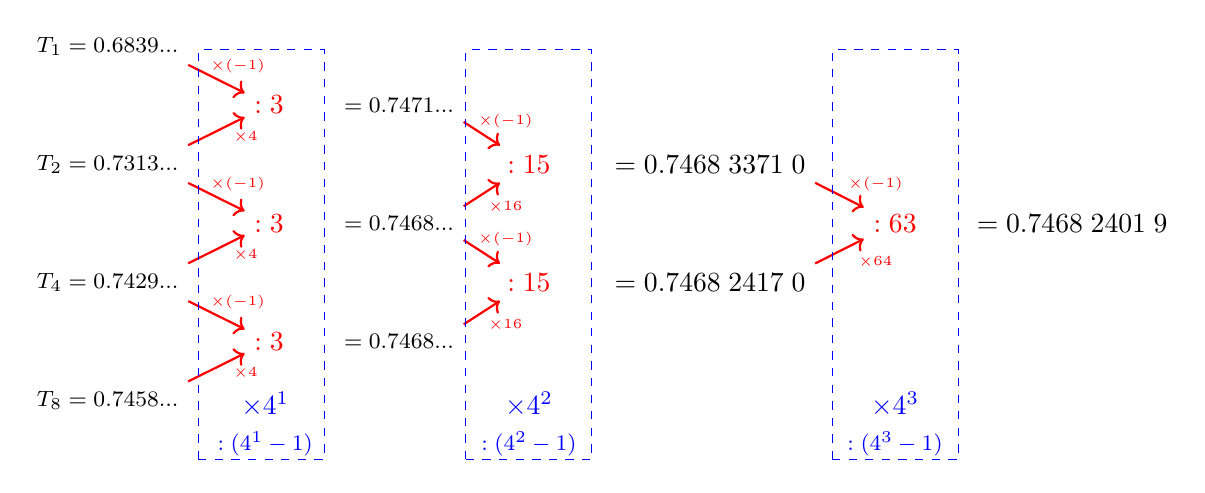
\begin{tikzpicture}


	\node (T1) at (0.75,5.25) {\footnotesize{$T_1 = 0.6839...$}};
	\node (T2) at (0.75,3.75) {\footnotesize{$T_2 = 0.7313...$}};
	\node (T4) at (0.75,2.25) {\footnotesize{$T_4 = 0.7429...$}};
	\node (T8) at (0.75,0.75) {\footnotesize{$T_8 = 0.7458...$}}; %Some uncertainty about last 2 digits.  Maybe recalculate in MATLAB
	\node (A1)[red] at (2.8, 4.5){$:3$};
	\node (A2)[red] at (2.8, 3){$:3$};
	\node (A3)[red] at (2.8, 1.5){$:3$};
	
	\node (B1)at (4.45,4.5){\footnotesize{$= 0.7471...$}};
	\node (B2) at (4.45,3){\footnotesize{$= 0.7468...$}};
	\node (B3) at (4.45,1.5){\footnotesize{$= 0.7468...$}};
	\node (D1)[red] at (6.1, 3.75){$:15$};
	\node (D2)[red] at (6.1, 2.25){$:15$};
	
	\node (E1) at (8.4,3.75){$= 0.7468\;3371\;0$};
	\node (E2) at (8.4,2.25){$= 0.7468\;2417\;0$};
	
	\node (F1)[red] at (10.75, 3){$:63$};
	\node (G1) at (13,3){$= 0.7468\;2401\;9$};

	\draw [->, thick,red] (T1.south east) to (A1);
	\draw [->, thick,red] (T2.north east) to (A1);
	\draw [->, thick,red] (T2.south east) to (A2);
	\draw [->, thick,red] (T4.north east) to (A2);
	\draw [->, thick,red] (T4.south east) to (A3);
	\draw [->, thick,red] (T8.north east) to (A3);

	\draw [->, thick,red] (B1.south east) to (D1);
	\draw [->, thick,red] (B2.north east) to (D1);
	\draw [->, thick,red] (B2.south east) to (D2);
	\draw [->, thick,red] (B3.north east) to (D2);
	\draw [->, thick,red] (E1.south east) to (F1);
	\draw [->, thick,red] (E2.north east) to (F1);
	
	\draw[draw=blue, dashed] (1.9,0) rectangle ++(1.6,5.2);
	\draw[draw=blue, dashed] (5.3,0) rectangle ++(1.6,5.2);
	\draw[draw=blue, dashed] (9.95,0) rectangle ++(1.6,5.2);
	
	\node (A1a)[red] at (2.4,5){\tiny{$\times (-1)$}};
	\node (A1b)[red] at (2.5,4.1){\tiny{$\times 4$}};
	\node (A2a)[red] at (2.4,3.5){\tiny{$\times (-1)$}};	
	\node (A2b)[red] at (2.5,2.6){\tiny{$\times 4$}};
	\node (A3a)[red] at (2.4,2){\tiny{$\times (-1)$}};	
	\node (A3b)[red] at (2.5,1.1){\tiny{$\times 4$}};

	\node (D1a)[red] at (5.8,4.3){\tiny{$\times (-1)$}};
	\node (D1b)[red] at (5.8,3.2){\tiny{$\times 16$}};
	\node (D2a)[red] at (5.8,2.8){\tiny{$\times (-1)$}};
	\node (D2b)[red] at (5.8,1.7){\tiny{$\times 16$}};
	\node (F1a)[red] at (10.5,3.5){\tiny{$\times (-1)$}};
	\node (F1b)[red] at (10.5,2.5){\tiny{$\times 64$}};
	
	\node (H1a)[blue] at (2.75,0.7){$\times 4^1$};
	\node (H2a)[blue] at (6.1,0.7){$\times 4^2$};
	\node (H3a)[blue] at (10.75,0.7){$\times 4^3$};

	\node (H1b)[blue] at (2.75,0.2){\footnotesize{$:(4^1-1)$}};
	\node (H2b)[blue] at (6.1,0.2){\footnotesize{$:(4^2-1)$}};
	\node (H3b)[blue] at (10.75,0.2){\footnotesize{$:(4^3-1)$}};
	
\normalsize	
\end{tikzpicture}
\end{center}

	Where do the powers of 4 come from? Using Taylor series, it can be shown that:\\
	$$ T(h)= \int^b_a f(x) dx - \!\!\!\!\! \underbrace{C_1 h^2}_{Dominating} \!\!\!\!-\; C_2 h^4 - C_3 h^6 $$
	
	$$ T(\frac{1}{2}) = \int^b_a f(x) dx - \tilde{C}_1 \frac{h^2}{4} - \tilde{C}_2 \frac{h^4}{16} - \tilde{C}_3 \frac{h^6}{64} - ...$$
	
	\noindent The smaller the $h$, the closer $C_1 \approx \tilde{C}_1$, $C_2 \approx \tilde{C}_2$...
	
	$$ \frac{4T(\frac{h}{2})-T(h)}{3} =  \int^b_a f(x) dx 
	\!\!\!\!\!\!\!\!\!\!\!\! \underbrace{\qquad \qquad}_{\text{eliminates dominating term}} \!\!\!\!\!\!\!\!\!
	 - \quad \underbrace{\frac{\tilde{C}_2 \frac{h^4}{4}+C_2 h^4}{3}}_{C_2 \frac{5}{12}h^4}$$


	Also worth noting is that because neighboring values are multiplied by $-1$ and a power of $4$, we do not need to worry about round-off errors
	 from subtracting similar values.

	
	\chapter{Solving Non-Linear Equations}
	
	\noindent \textit{Previously:}\\
	\underline{Bisection Method}:  We want to find zeros of a function, $f(x) = 0$.	We need an interval with a sign change:
	
	$$ f(a) \cdot f(b) < 0 $$
	
	\medskip
	\noindent $f$ must be continuous (Intermediate Value Theorem)

\begin{multicols}{2}
\begin{tikzpicture}
    \begin{axis}[
        legend pos=south east,
        axis x line=middle,
        axis y line=middle,
	xticklabels=\empty,
	yticklabels= \empty,
        grid = none ,
        width=7cm,
        height=3cm,
        grid style={dashed, gray!1},
        xmin=0,     % start the diagram at this x-coordinate
        xmax=8,    % end   the diagram at this x-coordinate
        ymin=-1,     % start the diagram at this y-coordinate
        ymax= 1,   % end   the diagram at this y-coordinate
        xlabel=$x$,
        ylabel=$y$,
        enlargelimits=true,
        tension=0.08]

  \addplot[red, only marks, mark=*] coordinates {(0,-1)(8,1)};
 \node(a) at (axis cs: 4,-0.6){\large{$\frac{a+b}{2}$}};
    \end{axis}
\end{tikzpicture}

	Compute function values of midpoint.
	\columnbreak
	
	$$f\Big( \frac{a+b}{2} \Big) = 0 \Rightarrow \text{done}\quad \! \! \qquad$$
	$$ f\Big( \frac{a+b}{2} \Big) > 0 \Rightarrow \text{keep going}$$
	$$ f\Big( \frac{a+b}{2} \Big) < 0 \Rightarrow \text{keep going}$$
\end{multicols}
	
	In the case that the midpoint value is greater than or less than zero, repeat the process with the sub-interval with the sign change, and
	repeat until the required accuracy is reached.
	
\begin{center}
	10 steps $\longrightarrow 2^{10} = 1024 \longrightarrow$ 3 digits
\end{center}

	Problems can occur in machine calculations, because of the gaps in the number system and because of roundoff errors in function evaluations.
	When ``$f(x)=$ close to zero'', we do not know if this is a roundoff error or really a value different from zero.
	
\pagebreak

\section{Newton's Method}
\begin{multicols}{2}
	\noindent $f(x)=0$\\
	$f$ is differentiable\\
	$x_0$ first guess\\
	\\
	\noindent Improved guess:
	$$ y = f(x_0) + f^\prime (x_2) \cdot (x-x_0) $$\\
	
	\noindent Continue until the desired accuracy is reached. (Look for some digits in successive guesses), or until it becomes obvious that the
	method fails.\\


\begin{tikzpicture}
    \begin{axis}[
        legend pos=south east,
        axis x line=middle,
        axis y line=middle,
	every axis x label/.style={at={(current axis.right of origin)},anchor=north},
	every axis y label/.style={at={(current axis.above origin)},anchor=east},
	xticklabels=\empty,
	yticklabels=\empty
        grid = none ,
        width=8cm,
        height=8cm,
        grid style={dashed, gray!1},
        xmin=0,
        xmax= 1.5,
        ymin=-0.25,
        ymax= 1.3,
        xlabel=x,
        ylabel=y,
        enlargelimits=true,
        tension=0.08]
        
        \addplot[domain=0.15:8, blue, thick,samples=250] {(x+0.25)^2/2 -0.5}; % Parabola
        \addplot[domain=0.7:1.65, red, thick,samples=250] {1.5*x-1.25}; % Tangent Line


	\addplot[dashed,red,mark=none] coordinates{(1.25,0)(1.25,0.625)} node[below, pos=0] {$x_0$}; %x0
	\addplot[red, only marks, mark=*] coordinates {(0.8333,0)(1.25,0.625)};
		\node(x1)[red] at (axis cs: 0.9,-0.06){{$x_1$}};


    \end{axis}
\end{tikzpicture}

\end{multicols}
	
	This method can go wrong.  Look at the function first!
	
\begin{multicols}{2}

\begin{tikzpicture}
    \begin{axis}[
        legend pos=south east,
        axis x line=middle,
        axis y line=middle,
	every axis x label/.style={at={(current axis.right of origin)},anchor=north},
	every axis y label/.style={at={(current axis.above origin)},anchor=east},
	xticklabels=\empty,
	yticklabels=\empty
        grid = none ,
        width=7cm,
        height=7cm,
        grid style={dashed, gray!1},
        xmin=0,     % start the diagram at this x-coordinate
        xmax= 1.5,    % end   the diagram at this x-coordinate
        ymin=-0.25,     % start the diagram at this y-coordinate
        ymax= 1.3,   % end   the diagram at this y-coordinate
        xlabel=x,
        ylabel=y,
        enlargelimits=true,
        tension=0.08]

        \addplot[domain=-0:8, blue, thick,samples=250] {2*(x-0.75)^2 + 0.1}; % Parabola

	\node(x1)[red] at (axis cs: 0.75,-0.2){{No Zeros!}};
    \end{axis}
\end{tikzpicture}


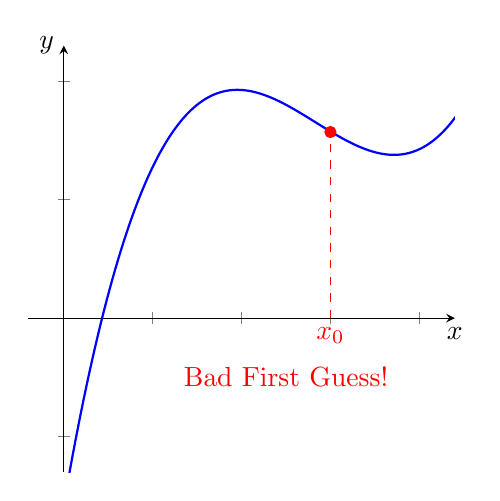
\begin{tikzpicture}
    \begin{axis}[
        legend pos=south east,
        axis x line=middle,
        axis y line=middle,
	every axis x label/.style={at={(current axis.right of origin)},anchor=north},
	every axis y label/.style={at={(current axis.above origin)},anchor=east},
	xticklabels=\empty,
	yticklabels=\empty
        grid = none ,
        width=7cm,
        height=7cm,
        grid style={dashed, gray!1},
        xmin=0,     % start the diagram at this x-coordinate
        xmax= 4,    % end   the diagram at this x-coordinate
        ymin=-1,     % start the diagram at this y-coordinate
        ymax= 2,   % end   the diagram at this y-coordinate
        xlabel=$x$,
        ylabel=$y$,
        enlargelimits=true,
        tension=0.08]

        \addplot[domain=-0:8,blue, thick,samples=250] {0.2*((x-2.5)^3-(x-1.5)^2)+2}; % Parabola


	\addplot[dashed,red,mark=none] coordinates{(3,0)(3,1.57)} node[below, pos=0] {$x_0$}; %x0
	\addplot[red, only marks, mark=*] coordinates {(3,1.57)};
		\node(x1)[red] at (axis cs: 2.5,-0.5){{Bad First Guess!}};


    \end{axis}
\end{tikzpicture}

\end{multicols}	
	
\section{Solving Fixed Point Equations}

	Another common type of equation is
	$$x = g(x)$$
	\noindent This is a fixed point equation.
	$$0 = g(x) - x \;\; \text{\small{when}} \;\; x \neq 0  \quad \Rightarrow \quad 1 = \frac{g(x)}{x} \Rightarrow 0 = \frac{g(x)}{x}-1$$\\
	
	\noindent Reflecting on Newton's Method:
	$$x_{n+1} =  x_n-\frac{f(x_n)}{f^\prime(x_n)} \quad \text{\small{when}} \quad \lim\limits_{n \to \infty}
	x_* \quad \text{\small{then}} \quad \underbrace{ x_* = x_* - \frac{f(x_*)}{f^\prime (x_*)}}_{g(x_*)}$$\\
	
	
	\pagebreak
	\noindent \textbf{Example:} $x= \cos x$
	
\begin{center}	
\begin{tikzpicture}
    \begin{axis}[
        legend pos=south east,
        axis x line=middle,
        axis y line=middle,
	every axis x label/.style={at={(current axis.right of origin)},anchor=north},
	every axis y label/.style={at={(current axis.above origin)},anchor=east},
	xticklabels=\empty,
	yticklabels=\empty
        grid = none,
        width=12cm,
        height=5.8cm,
        grid style={dashed, gray!1},
        xmin=-1.1,     % start the diagram at this x-coordinate
        xmax= 4.3,    % end   the diagram at this x-coordinate
        ymin=-1.25,     % start the diagram at this y-coordinate
        ymax= 1.25,   % end   the diagram at this y-coordinate
        xlabel=x,
        ylabel=y,
        enlargelimits=true,
        tension=0.08]

        \addplot[domain=-1.57:4.71,blue, thick,samples=250] {cos(deg(x))};
        \addplot[domain=-1:2, gray, thick,samples=250] {x};


	\addplot[dashed,red,mark=none] coordinates{(0.7,0)(0.7,0.765)} node[below, pos=0] {$x_0$}; %x0
	\addplot[red, only marks, mark=*] coordinates {(0.7,0.765)};
	\node(x1)[blue] at (axis cs: 2.5,0.5){{$y = \cos x  $}};
    \end{axis}
\end{tikzpicture}
\end{center}

	\noindent First guess: $x_0 = 0.7$. Apply Fixed Point Iteration:
	$$ x_{n+1} \cos(x_n), \quad n = 0, 1, 2,...$$
	$$ \cos (0.7) = 0.76484219... $$

\begin{center}
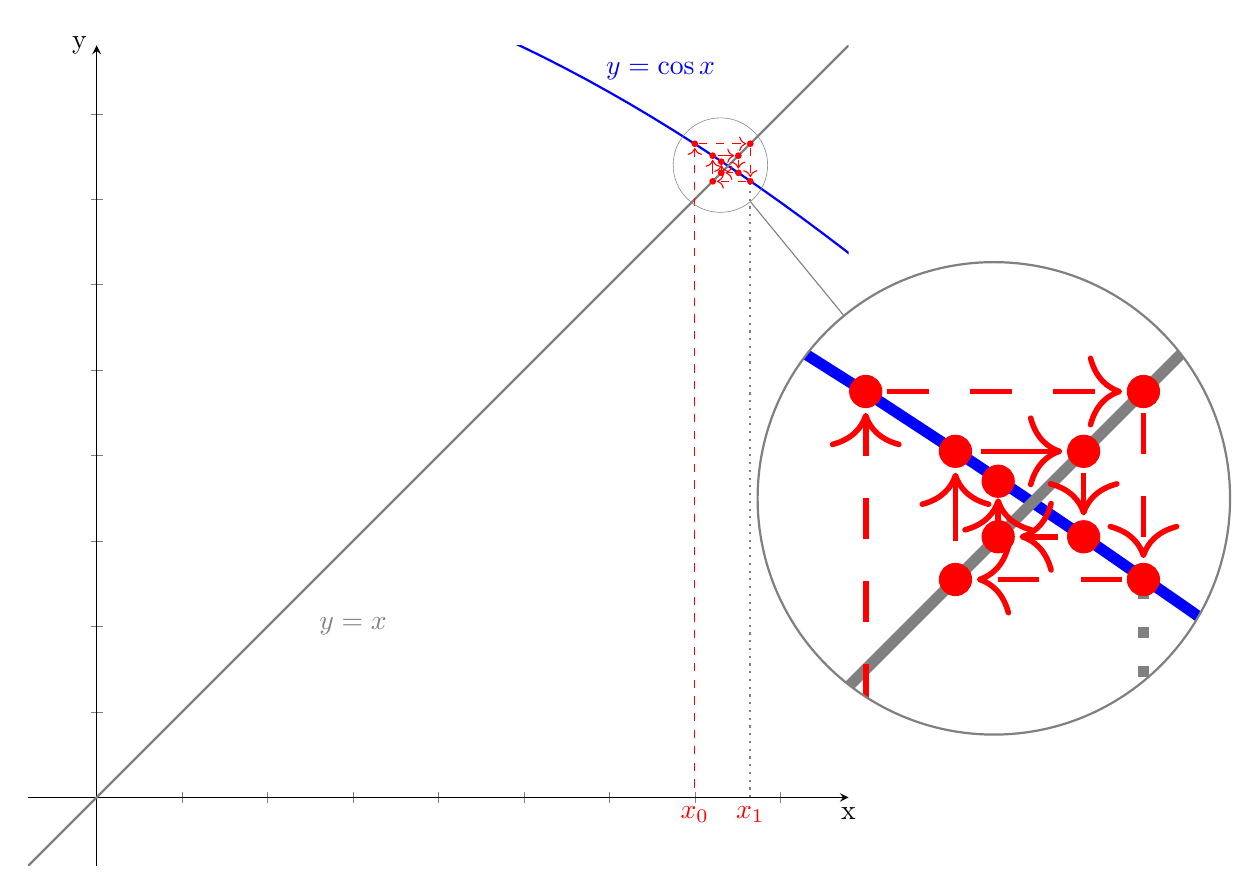
\begin{tikzpicture}[spy using outlines=
	{circle, magnification=5, connect spies}]
    \begin{axis}[
        legend pos=south east,
        axis x line=middle,
        axis y line=middle,
	every axis x label/.style={at={(current axis.right of origin)},anchor=north},
	every axis y label/.style={at={(current axis.above origin)},anchor=east},
	xticklabels=\empty,
	yticklabels=\empty
        grid = none,
        width=12cm,
        height=12cm,
        grid style={dashed, gray!1},
        xmin=0,     % start the diagram at this x-coordinate
        xmax= 0.8,    % end   the diagram at this x-coordinate
        ymin=0,     % start the diagram at this y-coordinate
        ymax= 0.8,   % end   the diagram at this y-coordinate
        xlabel=x,
        ylabel=y,
        enlargelimits=true,
        tension=0.08]

        \addplot[domain=-1.57:4.71,blue, thick,samples=250] {cos(deg(x))};
        \addplot[domain=-1:2, gray, thick,samples=250] {x};


%	\addplot[dashed,red,mark=none] coordinates{(0.7,0)(0.7,0.765)} node[below, pos=0] {$x_0$}; %x0
	
	\addplot[red, only marks, mark=*, mark size=1pt] coordinates {(0.7,0.765)(0.765,0.765)(0.765, 0.721)(0.721,0.721)(0.721,0.751)(0.751,0.751)(0.751,0.731)(0.731,0.731)(0.731,0.744)};
	\node(cX)[blue] at (axis cs: 0.66,0.85){{$y = \cos x  $}};
	\node(yX)[gray] at (axis cs: 0.3,0.2){{$y = x  $}};


	\node[red] (y0) at (axis cs: 0.7,0){};
	\node[red] (x0) at (axis cs: 0.7,0.765){};
	\node[red] (y1) at (axis cs: 0.765,0.765){};
	\node[red] (x1) at (axis cs: 0.765,0.721){};
	\node[red] (y2) at (axis cs: 0.721,0.721){};
	\node[red] (x2) at (axis cs: 0.721,0.751){};
	\node[red] (y3) at (axis cs: 0.751,0.751){};
	\node[red] (x3) at (axis cs: 0.751,0.735){};
	
	\node[red] (x_0) at (axis cs: 0.7, -0.02){$x_0$};
	\node[red] (x_1) at (axis cs: 0.765, -0.02){$x_1$};
	\addplot[dotted,gray,thick,mark=none] coordinates{(0.765,0)(0.765,0.721)} node[below, pos=0] {};
		
	\draw[red, dashed, ->](y0)--(axis cs: 0.7, 0.76);
	\draw[red, dashed, ->](axis cs: 0.705,0.765)--(axis cs: 0.76, 0.765);
	\draw[red, dashed, ->](axis cs: 0.765, 0.76)--(axis cs: 0.765, 0.726);
	\draw[red, dashed, ->](axis cs: 0.76, 0.721)--(axis cs: 0.726, 0.721);
	\draw[red, ->](axis cs: 0.721, 0.73)--(axis cs: 0.721, 0.746);
	\draw[red, ->](axis cs: 0.727, 0.751)--(axis cs: 0.746, 0.751);
	\draw[red, ->](axis cs: 0.751,0.746)--(axis cs: 0.751, 0.736);
	\draw[red, ->](axis cs:0.745,0.731)--(axis cs: 0.736, 0.731);
	\draw[red, ->](axis cs:0.731,0.731)--(axis cs: 0.731, 0.74);
		
	\coordinate (spypoint) at (axis cs:0.73,0.74);
	\coordinate (magnifyglass) at (axis cs:1.05,0.35);
	
	\spy [gray, size=6cm] on (spypoint)
   in node[fill=white] at (magnifyglass);
    \end{axis}
\end{tikzpicture}
	$$ y_1 = \cos x_0 \qquad x_1 = y_1 \qquad y_2 = \cos x_1 \qquad x_2 = y_2 \qquad y_3 = \cos x_2 \qquad x_3 = y_3 $$\\
	\bigskip
\fbox
{
	\parbox{0.6\textwidth}
	{
		\noindent \textit{\underline{Fixed Point Iteration}:}\\
		\vspace{-3mm}
		\\
			To solve $x = g(x)$, try $x_0$ (first guess)
			$$x_{n+1} = g(x_n), n = 0, 1, 2, ...$$
			until the method converges or shows that it does not work.
	}
}

\end{center}
	\noindent \textit{When does it work?} In case it works, when is it fast or slow?
	
\begin{multicols}{2}
\begin{center}
% [BEGIN CHART 1] -------------------------------------------------------------------------------------------------------------------------------------------------------------

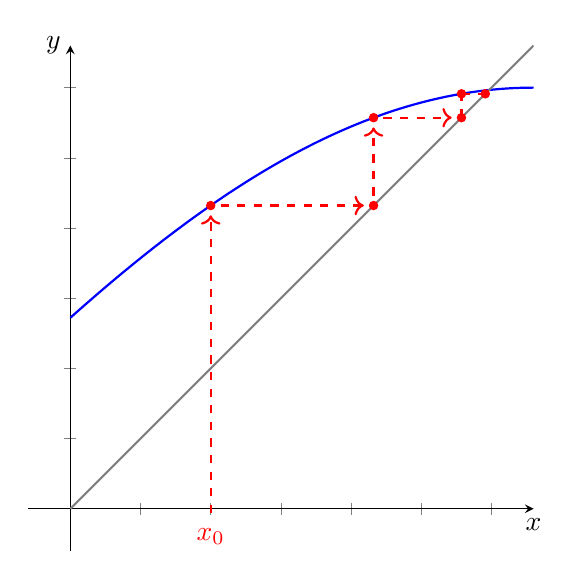
\begin{tikzpicture}
    \begin{axis}[
        legend pos=south east,
        axis x line=middle,
        axis y line=middle,
	every axis x label/.style={at={(current axis.right of origin)},anchor=north},
	every axis y label/.style={at={(current axis.above origin)},anchor=east},
	xticklabels=\empty,
	yticklabels=\empty
        grid = none ,
        width=8cm,
        height=8cm,
        grid style={dashed, gray!1},
        xmin=0,     % start the diagram at this x-coordinate
        xmax= 3,    % end   the diagram at this x-coordinate
        ymin=0,     % start the diagram at this y-coordinate
        ymax= 3,   % end   the diagram at this y-coordinate
        xlabel=$x$,
        ylabel=$y$,
        enlargelimits=true,
        tension=0.08]

        \addplot[domain=-0:8,blue, thick,samples=250] {3*cos(deg(x/3-1.1))}; % Parabola
         \addplot[domain=-0:8, gray, thick,samples=250] {x};

	\node[red] (x0) at (axis cs: 1,-0.1){};
	\node[red] (y0) at (axis cs: 1,2.16){};
	\node[red] (x1) at (axis cs: 2.16,2.16){};
	\node[red] (y1) at (axis cs: 2.16,2.786){};
	\node[red] (x2) at (axis cs: 2.786,2.786){};
	\node[red] (y2) at (axis cs: 2.786,2.956){};
	\node[red] (x3) at (axis cs: 2.956,2.956){};
	\node[red] (y3) at (axis cs: 2.956,2.98){};
	\node[red] (xL) at (axis cs: 1,-0.2){$x_0$};

	\draw[red, dashed, thick, ->](x0)--(y0);
	\draw[red, dashed, thick, ->](y0)--(x1);
	\draw[red, dashed, thick, ->](x1)--(y1);
	\draw[red, dashed, thick, ->](y1)--(x2);
	\draw[red, dashed, thick](x2.center)--(y2.center);
	\draw[red, dashed, thick](y2.center)--(x3.center);
	\draw[red, dashed, thick](x3.center)--(y3.center);

	\addplot[red, only marks, mark=*, mark size=1.5pt] coordinates {(1,2.16)(2.16,2.16)(2.16,2.786)(2.786,2.786)(2.786,2.956)(2.956,2.956)};

    \end{axis}
\end{tikzpicture}

	\noindent \textbf{Converging ``Staircase''}\\
	\vspace{1cm}

% ------------------------------------------------------------------------------------------------------------------------------------------------------------- [END CHART 1]



% [BEGIN CHART 3] -------------------------------------------------------------------------------------------------------------------------------------------------------------
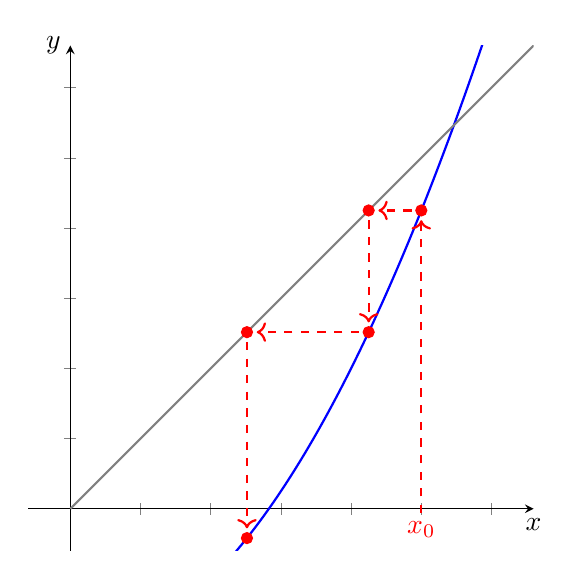
\begin{tikzpicture}
    \begin{axis}[
        legend pos=south east,
        axis x line=middle,
        axis y line=middle,
	every axis x label/.style={at={(current axis.right of origin)},anchor=north},
	every axis y label/.style={at={(current axis.above origin)},anchor=east},
	xticklabels=\empty,
	yticklabels=\empty
        grid = none ,
        width=8cm,
        height=8cm,
        grid style={dashed, gray!1},
        xmin=0,     % start the diagram at this x-coordinate
        xmax= 3,    % end   the diagram at this x-coordinate
        ymin=0,     % start the diagram at this y-coordinate
        ymax= 3,   % end   the diagram at this y-coordinate
        xlabel=$x$,
        ylabel=$y$,
        enlargelimits=true,
        tension=0.08]

        \addplot[domain=-0:8,blue, thick,samples=250] {0.5*x^2-1}; % Parabola
         \addplot[domain=-0:8, gray, thick,samples=250] {x};
	
	\node[red] (x0) at (axis cs: 2.5,-0.1){};
	\node[red] (y0) at (axis cs: 2.5,2.125){};
	\node[red] (x1) at (axis cs: 2.125,2.125){};
	\node[red] (y1) at (axis cs: 2.125,1.258){};
	\node[red] (x2) at (axis cs: 1.258,1.258){};
	\node[red] (y2) at (axis cs: 1.258,-0.209){};
	\node[red] (xL) at (axis cs: 2.5,-0.15){$x_0$};
	
	\draw[red, dashed, thick, ->](x0)--(y0);
	\draw[red, dashed, thick, ->](y0)--(x1);
	\draw[red, dashed, thick, ->](x1)--(y1);
	\draw[red, dashed, thick, ->](y1)--(x2);
	\draw[red, dashed, thick, ->](x2)--(y2);
	
	\addplot[red, only marks, mark=*, mark size=2pt] coordinates {(2.5,2.125)(2.125,2.125)(2.125,1.258)(1.258,1.258)(1.258,-0.209)};
	
    \end{axis}
\end{tikzpicture}

	\noindent \textbf{Diverging Staircase}\\
% ------------------------------------------------------------------------------------------------------------------------------------------------------------- [END CHART 3]



% [BEGIN CHART 2] -------------------------------------------------------------------------------------------------------------------------------------------------------------
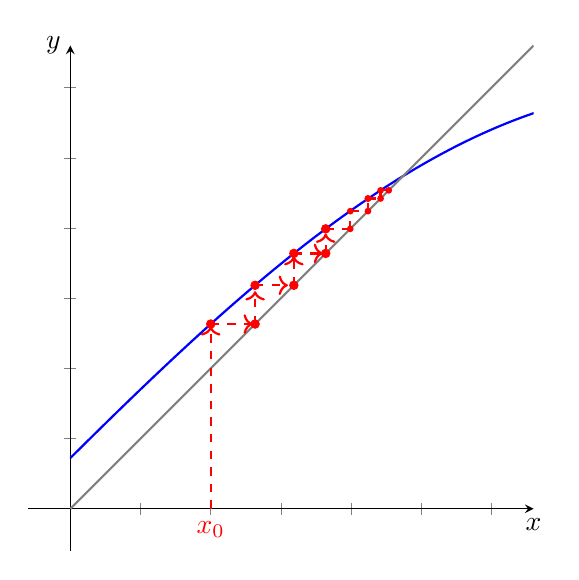
\begin{tikzpicture}
    \begin{axis}[
        legend pos=south east,
        axis x line=middle,
        axis y line=middle,
	every axis x label/.style={at={(current axis.right of origin)},anchor=north},
	every axis y label/.style={at={(current axis.above origin)},anchor=east},
	xticklabels={\hspace{-5mm}5,\hspace{-5mm}6},
	yticklabels=\empty
        grid = none ,
        width=8cm,
        height=8cm,
        grid style={dashed, gray!1},
        xmin=0,     % start the diagram at this x-coordinate
        xmax= 3,    % end   the diagram at this x-coordinate
        ymin=0,     % start the diagram at this y-coordinate
        ymax= 3,   % end   the diagram at this y-coordinate
        xlabel=$x$,
        ylabel=$y$,
        enlargelimits=true,
        tension=0.08]

        \addplot[domain=-0:8,blue, thick,samples=250] {3*cos(deg(x/3-1.45))}; % Parabola
         \addplot[domain=-0:8, gray, thick,samples=250] {x};

	\draw[red, dashed, thick, ->](axis cs: 1,0)--(axis cs:1,1.3);
	\draw[red, dashed, thick, ->](axis cs: 1,1.316)--(axis cs: 1.3,1.316);	
	\draw[red, dashed, thick, ->](axis cs: 1.316,1.316)--(axis cs: 1.316,1.55);
	\draw[red, dashed, thick, ->](axis cs: 1.316,1.592)--(axis cs: 1.55,1.592);
	\draw[red, dashed, thick, ->](axis cs: 1.592,1.592)--(axis cs: 1.592,1.8);
	\draw[red, dashed, thick, ->](axis cs: 1.592,1.819)--(axis cs: 1.8,1.819);
	\draw[red, dashed, thick, ->](axis cs: 1.819,1.819)--(axis cs: 1.819,1.96);

	\addplot[dashed,red,thick,mark=none] coordinates{(1.819,1.994)(1.994,1.994)} node[below, pos=0] {};
	\addplot[dashed,red,thick,mark=none] coordinates{(1.994,1.994)(1.994,2.12)} node[below, pos=0] {};
	\addplot[dashed,red,thick,mark=none] coordinates{(1.994,2.12)(2.12,2.12)} node[below, pos=0] {};
	\addplot[dashed,red,thick,mark=none] coordinates{(2.12,2.12)(2.12,2.21)} node[below, pos=0] {};
	\addplot[dashed,red,thick,mark=none] coordinates{(2.12,2.21)(2.21,2.21)} node[below, pos=0] {};
	\addplot[dashed,red,thick,mark=none] coordinates{(2.21,2.21)(2.21,2.268)} node[below, pos=0] {};
	\addplot[dashed,red,thick,mark=none] coordinates{(2.21,2.268)(2.268,2.268)} node[below, pos=0] {};
	
	\addplot[red, only marks, mark=*, mark size=1.5pt] coordinates {(1,1.316)(1.316,1.316)(1.316,1.592)(1.592,1.592)(1.592,1.819)(1.819,1.819)(1.819,1.994)};
	\addplot[red, only marks, mark=*, mark size=1pt] coordinates {(1.994,1.994)(1.994,2.12)(2.12,2.12)(2.12,2.21)(2.12,2.21)(2.21,2.21)(2.21,2.268)(2.268,2.268)};
	
	\node[red] (xL) at (axis cs: 1,-0.15){$x_0$};
    \end{axis}
\end{tikzpicture}

	\noindent \textbf{Slow Converging Staircase}
	\vspace{1cm}

% ------------------------------------------------------------------------------------------------------------------------------------------------------------- [END CHART 2]




% [BEGIN CHART 4]-------------------------------------------------------------------------------------------------------------------------------------------------------------
\begin{tikzpicture}
    \begin{axis}[
        legend pos=south east,
        axis x line=middle,
        axis y line=middle,
	every axis x label/.style={at={(current axis.right of origin)},anchor=north},
	every axis y label/.style={at={(current axis.above origin)},anchor=east},
	xticklabels=\empty,
	yticklabels=\empty
        grid = none ,
        width=8cm,
        height=8cm,
        grid style={dashed, gray!1},
        xmin=0,     % start the diagram at this x-coordinate
        xmax= 3.5,    % end   the diagram at this x-coordinate
        ymin=0,     % start the diagram at this y-coordinate
        ymax= 3.5,   % end   the diagram at this y-coordinate
        xlabel=$x$,
        ylabel=$y$,
        enlargelimits=true,
        tension=0.08]

        \addplot[domain=0:3.5,blue, thick,samples=250] {4*cos(deg(x/2))+1}; % Parabola
         \addplot[domain=-0:8, gray, thick,samples=250] {x};

	
	\node[red] (x0) at (axis cs: 2.5,0){};
	\node[red] (y0) at (axis cs: 2.5,2.26){};
	\node[red] (x1) at (axis cs: 2.26,2.26){};
	\node[red] (y1) at (axis cs: 2.26,2.704){};
	\node[red] (x2) at (axis cs: 2.704,2.704){};
	\node[red] (y2) at (axis cs: 2.704,1.868){};
	\node[red] (x3) at (axis cs: 1.868,1.868){};
	\node[red] (y3) at (axis cs: 1.868,3.379){};
	\node[red] (x4) at (axis cs: 3.379,3.379){};
	\node[red] (y4) at (axis cs: 3.379,0.526){};
	
	\node[red] (xL) at (axis cs: 2.5,-0.2){$x_0$};
	
	\draw[red, dashed, thick, ->](x0)--(y0);
	\draw[red, dashed, thick, ->](y0)--(x1);
	\draw[red, dashed, thick, ->](x1)--(y1);
	\draw[red, dashed, thick, ->](y1)--(x2);
	\draw[red, dashed, thick, ->](x2)--(y2);
	\draw[red, dashed, thick, ->](y2)--(x3);
	\draw[red, dashed, thick, ->](x3)--(y3);
	\draw[red, dashed, thick, ->](y3)--(x4);
	\draw[red, dashed, thick, ->](x4)--(y4);	
	
	
	\addplot[red, only marks, mark=*, mark size=2pt] coordinates {(2.5,2.26)(2.26,2.26)(2.26,2.704)(2.704,2.704)(2.704,1.868)(1.868,1.868)(1.868,3.379)(3.379,3.379)(3.379,0.526)};
	
    \end{axis}
\end{tikzpicture}
\noindent \textbf{Diverging Spiral}\\
%--------------------------------------------------------------------------------------------------------------------------------------------------------------------[END CHART 4]


\end{center}
\end{multicols}
	
\begin{center}
	Slope between $ -1 < s < 1 \Rightarrow \text{convergent}$
\end{center}
	
	\noindent If $g$ is differentiable, the fixed point iteration works when $ \lvert g^\prime \rvert <1 $ for all $x$ in that
	 neighborhood and if the initial guess is also in that neighborhood.
	
\begin{center}
	$g^\prime > 0 \Rightarrow$ ``Staircase''\\
	\medskip
	\hspace{-7.5mm} $g^\prime < 0 \Rightarrow$ ``Spiral''
\end{center}

	\noindent The closer  $ \lvert g^\prime \rvert$ is to 1, the slower the convergence. In the spiral case we can use averaging to
	 accelerate the convergence.

\begin{center}
\begin{tikzpicture}
    \begin{axis}[
        legend pos=south east,
        axis x line=middle,
        axis y line=middle,
	every axis x label/.style={at={(current axis.right of origin)},anchor=north},
	every axis y label/.style={at={(current axis.above origin)},anchor=east},
	xticklabels=\empty,
	yticklabels=\empty
        grid = none ,
        width=7cm,
        height=7cm,
        grid style={dashed, gray!1},
        xmin=0,     % start the diagram at this x-coordinate
        xmax= 2,    % end   the diagram at this x-coordinate
        ymin=0,     % start the diagram at this y-coordinate
        ymax= 2,   % end   the diagram at this y-coordinate
        xlabel=$x$,
        ylabel=$y$,
        enlargelimits=true,
        tension=0.08]

        \addplot[domain=-0:2.5,blue, thick,samples=250] {log2(x+1.5)};
        \addplot[domain=-0:2,red, thick,samples=250] {pow(2,x)-1.5};
         \addplot[domain=-0:2, gray, thick,samples=250] {x};

	\node[blue] (x0) at (axis cs: 1.1,1.7){$g^{-1}(x)=x$};
    \end{axis}
\end{tikzpicture}
	\linebreak
	Take the inverse function.
\end{center}

	\noindent\textbf{Example:} $x = \tan x$
	
\begin{center}
\begin{tikzpicture}
    \begin{axis}[
        legend pos=south east,
        axis x line=middle,
        axis y line=middle,
	every axis x label/.style={at={(current axis.right of origin)},anchor=north},
	every axis y label/.style={at={(current axis.above origin)},anchor=east},
   	xtick = {-4.712389, -3.14159, ..., 4.712389},
	xticklabels=\empty,
	yticklabels=\empty
        grid = none ,
        width=9cm,
        height=9cm,
        grid style={dashed, gray!1},
        xmin=-4.6,     % start the diagram at this x-coordinate
        xmax= 4.6,    % end   the diagram at this x-coordinate
        ymin=-4.6,     % start the diagram at this y-coordinate
        ymax=4.6,   % end   the diagram at this y-coordinate
        xlabel=$x$,
        ylabel=$y$,
        enlargelimits=true,
        tension=0.08]

         \addplot[domain=-5:5, gray, thick,samples=250] {x};
        \addplot[domain=-1.5:1.5,red, thick,samples=250] {tan(deg(x))};
        \addplot[domain=1.6:4.6,red, thick,samples=250] {tan(deg(x-3.14159))};
        \addplot[domain=-4.6:-1.6,red, thick,samples=250] {tan(deg(x+3.14159))};

	\draw[red, dashed](axis cs: 1.5708, -6)--(axis cs: 1.5708, 6);
	\draw[red, dashed](axis cs: -1.5708, -6)--(axis cs: -1.5708, 6);
	\draw[red, dashed](axis cs: -4.7124, -6)--(axis cs: -4.7124, 6);
	\draw[red, dashed](axis cs: 4.7124, -6)--(axis cs: 4.7124, 6);
	
	\node[red] (A1) at (axis cs: -2,-0.5){$- \frac{\pi}{2}$};
	\node[red] (A2) at (axis cs: 1.35,-0.5){$\frac{\pi}{2}$};
	\node[red] (A3) at (axis cs: -5.2,-0.5){$\frac{-3 \pi}{2}$};
	\node[red] (A4) at (axis cs: 4.4,-0.5){$\frac{3 \pi}{2}$};
    \end{axis}
\end{tikzpicture}
\end{center}
	We have infinitely many solutions.  One of them is $x = 0$.  The further we get from 0, the closer the value will get to 
	the vertical asymptotes.\\
	
	\noindent Let's find a solution close to $x = \frac{3 \pi}{2}$.  We need the inverse of the function to make fixed point iteration work.
	
\begin{multicols}{2}
	\begin{tikzpicture}
    \begin{axis}[
        legend pos=south east,
        axis x line=middle,
        axis y line=middle,
	every axis x label/.style={at={(current axis.right of origin)},anchor=north},
	every axis y label/.style={at={(current axis.above origin)},anchor=east},
	xticklabels=\empty,
	ytick = {-1.570796, 0, ..., 6.283185},
	yticklabels=\empty,
        grid = none ,
        width=8cm,
        height=8cm,
        grid style={dashed, gray!1},
        xmin=-1,     % start the diagram at this x-coordinate
        xmax= 5,    % end   the diagram at this x-coordinate
        ymin=-1,     % start the diagram at this y-coordinate
        ymax=5,   % end   the diagram at this y-coordinate
        xlabel=$x$,
        ylabel=$y$,
        enlargelimits=true,
        tension=0.08]

         \addplot[domain=-5:6, gray, thick,samples=250] {x};
        \addplot[domain=-5:6,blue, thick,samples=250] {rad(atan(x))};
        \addplot[domain=-5:6,blue, thick,samples=250] {rad(atan(x))+3.14159};

	\draw[blue, dashed](axis cs: -6,1.5708)--(axis cs: 6,1.5708);
	\draw[blue, dashed](axis cs: -6,4.71239)--(axis cs: 0.7,4.71239);
	\draw[blue, dashed](axis cs: 4.2,4.71239)--(axis cs: 6,4.71239);
	\draw[red, thick, ->](axis cs: 4.7,1.5)--(axis cs: 4.7, 4.4);
%	\draw[red, dashed](axis cs: -4.7124, -6)--(axis cs: -4.7124, 6);
%	\draw[red, dashed](axis cs: 4.7124, -6)--(axis cs: 4.7124, 6);
	
	\node[red] (A1) at (axis cs: 5.1,3){$+\pi$};
	\node[blue] (A2) at (axis cs: 2.5,4.8){$y = \tan^{-1} x + \pi$};
	\node[blue] (A3) at (axis cs: -0.25,1.2){$\frac{\pi}{2}$};
	\node[blue] (A4) at (axis cs: -0.25,4.3){$\frac{3 \pi}{2}$};
    \end{axis}
\end{tikzpicture}

	\noindent This problem works extremely well with fixed point iteration since the slope is almost horizontal.

	$$ 4.493 = \tan^{-1} 4.493 + \pi$$
	
	$\longrightarrow$ applying inverse function:
	
	$$ \tan(4.493... = \tan \big(\tan^{-1}(4.493)+\cancelto{\footnotesize{\pi- \text{periodic}}}{\pi} \big)$$
	$$ = \tan \big( \tan^{-1} (4.493) \big)$$
	\normalsize
	\noindent No need to go back to the original problem.
\end{multicols}

	\noindent \textbf{Example:}\\
	$$x^2 +y - 37 = 0$$
	$$x - y^2-5 = 0$$
	$$x+y+z-3=0$$\\


	\noindent Only the third equation involves $z$, so use the first and second to solve $(x,y)$.  Then plug the solutions in
	the corresponding z.

	\noindent One possibility: We can plug $y = 37 - x^2$ into the second equation and solve\\
	$$ x - (37 - x^2)^2 = 5 \longleftarrow \text{\footnotesize{(4th order equation)}}$$\\


\begin{center}
\begin{tikzpicture}
    \begin{axis}[
        legend pos=south east,
        axis x line=middle,
        axis y line=middle,
	every axis x label/.style={at={(current axis.right of origin)},anchor=north},
	every axis y label/.style={at={(current axis.above origin)},anchor=east},
	xticklabels=\empty,
	yticklabels=\empty
        grid = none ,
        width=14cm,
        height=14cm,
        grid style={dashed, gray!1},
        xmin=0,     % start the diagram at this x-coordinate
        xmax= 10,    % end   the diagram at this x-coordinate
        ymin=-2,     % start the diagram at this y-coordinate
        ymax= 40,   % end   the diagram at this y-coordinate
        xlabel=$x$,
        ylabel=$y$,
        enlargelimits=true,
        tension=0.08]

        \addplot[domain=-0:8,red, thick,samples=250] {37-x^2};
         \addplot[domain=-0:10, blue, thick,samples=250] {sqrt(x-5)};
         \addplot[domain=-0:10, blue, thick,samples=250] {-sqrt(x-5)};
	\node[red] (x0) at (axis cs: 5,30){$y = 37-x^2$};
	\node[blue] (y0) at (axis cs: 8,5){$y = \sqrt{x-5}$};

	
	\addplot[blue, only marks, mark=*, mark size=0.5pt] coordinates {(5,0)};
	\addplot[red, only marks, mark=*, mark size=1.5pt] coordinates {(6,1)(6.17,-1.1)};	
    \end{axis}
\end{tikzpicture}

\bigskip

\begin{tikzpicture}[spy using outlines=
	{circle, magnification=5, connect spies}]
    \begin{axis}[
        legend pos=south east,
        axis x line=middle,
        axis y line=middle,
	every axis x label/.style={at={(current axis.right of origin)},anchor=north},
	every axis y label/.style={at={(current axis.above origin)},anchor=east},
	xticklabels={\hspace{-5mm}5,\hspace{-5mm}6},
	yticklabels=\empty
        grid = none ,
        width=14cm,
        height=14cm,
        grid style={dashed, gray!1},
        xmin=4.9,     % start the diagram at this x-coordinate
        xmax= 7,    % end   the diagram at this x-coordinate
        ymin=-1.5,     % start the diagram at this y-coordinate
        ymax= 1.5,   % end   the diagram at this y-coordinate
        xlabel=$x$,
        ylabel=$y$,
        enlargelimits=true,
        tension=0.08]

        \addplot[domain=4.9:8,gray, thick,samples=250] {37-x^2}; % Parabola
        \addplot[domain=5:5.021, blue, thick,samples=250] {-6.9*(x-5};
         \addplot[domain=0:10, blue, thick,samples=250] {-sqrt(x-5)};
	
	\node[gray] (x0) at (axis cs: 6.2,1.7){$y = 37-x^2$};
	\node[blue] (y0) at (axis cs: 6.7,-1.1){$y = - \sqrt{x-5}$};	
	\node (n5) at (axis cs:5,0.1){5};
	\node (n6) at (axis cs:6,0.1){6};

	
	\draw[red, dashed, ->](axis cs:6,0)--(axis cs:6, -0.985);
	\draw[red, dashed, ->](axis cs:6,-1)--(axis cs:6.155, -1);
	\draw[red, dashed, ->](axis cs:6.165,-1.02)--(axis cs:6.165, -1.065);

	\addplot[red, only marks, mark=*, mark size=1pt] coordinates {(6,-1)(6.165,-1)(6.165, -1.078)};
	\addplot[gray, only marks, mark=*, mark size=1pt] coordinates {(6.17,-1.08)};	
	
	\coordinate (spypoint) at (axis cs:6.08,-1.05);
	\coordinate (magnifyglass) at (axis cs:5.35,1);
	
	\spy [gray, size=6cm] on (spypoint) in node[fill=white] at (magnifyglass);
    \end{axis}
\end{tikzpicture}
\end{center}
\bigskip
	
	\noindent Now, develop the method:
	
	$$ -1 = y_0 = 37 - x^2$$
	
	\noindent We need the positive solution.
	$$ x^2 = 37-y_0 $$
	
	

\end{document}	

